\documentclass[a4paper,12pt]{article}
% \documentclass[10pt, twocolumn]{article} % 缩小字体+双栏分页
\usepackage[paper=a4paper, margin=2cm]{geometry} % 调整页边距
\usepackage{amsmath}
\usepackage{array}
\usepackage{fancyhdr}
\usepackage{ctex}
\usepackage{graphicx}
\usepackage{float}
\usepackage{titlepic}
\usepackage{listings}
\usepackage{xcolor}      %代码着色宏包
\usepackage{CJK}         %显示中文宏包
\usepackage{booktabs}    %用于更美观的表格线
\usepackage{tabularx}    %自动调整列宽
\lstset{
    basicstyle=\ttfamily\footnotesize, % 缩小字号
    columns=fullflexible,              % 紧凑字符间距
    keywordstyle=\color{blue},         % 关键词高亮
    commentstyle=\color{gray},         % 注释颜色
    numbers=left,                      % 显示行号
    numberstyle=\tiny\color{gray},     % 行号字号
    frame=single,                      % 边框
    framesep=2pt,                      % 边框间距
    xleftmargin=10pt,                  % 左边距
    breaklines=true,                   % 自动换行
    language=C++,                      % c++
    postbreak=\mbox{\textcolor{red}{$\hookrightarrow$}\space}, % 换行标记
}

\titlepic{
\includegraphics[width=.7\linewidth]{IMG_1145.png}}
\title{XCPC 算法模版 Special}
\author{galiyu(1328063334@qq.com)}
\date{\today}

\begin{document}
\maketitle
\thispagestyle{empty}
\clearpage
\newpage

\pagestyle{fancy}
\fancyhead{}
\fancyfoot{}
\tableofcontents
\newpage

\fancyhead[R]{\thepage}
\fancyhead[L]{基础算法}

\section{基础算法}
\subsection{二分}

\noindent 有些时候 check 函数中一些变量可能会超出 i64 的范围, 为了防止这种情况发生, 
我们可以设置一个上界, 这些变量运算时与上界取 min。\\

\noindent 如果 \(l, r\) 有时候二分的时候经常死循环,
尤其是浮点二分,这个时候可以限定二分次数,一般是二分范围的 \(log_2\) 次。 

\begin{lstlisting}
// created on 24-8-23

// 整数二分(1)
int l = 0, r = n;
while (r > l){
    int mid = (l + r) / 2;
    if (check(mid)) r = mid;
    else l = mid + 1;
}
// 整数二分(2)
int l = 0, r = n;
while (r > l){
    int mid = (l + r + 1) / 2;
    if (check(mid)) l = mid;
    else r = mid - 1;
}
// 浮点二分
const double acc = 1e-6; // 设置精度
double l = 0, r = n;
while (r - l > acc){
    double mid = (l + r) / 2;
    if (check(mid)) r = mid;
    else l = mid;
}
\end{lstlisting}

\subsection{三分}

\noindent 通常是用于寻找某个函数的最值。

\begin{lstlisting}
// created on 24-8-23

//三分求f函数的最大值(定义域为整数)
int maximum_int(int L, int R) { 
    while (R > L) {
        int m1 = (2 * L + R) / 3;
        int m2 = (2 * R + L + 2) / 3;
        if (f(m1) > f(m2)) R = m2 - 1;
        else L = m1 + 1;
    }
    return L; //f(L)为最大值
}
//三分求f函数的最小值(定义域为整数)
int minimun_int(int L, int R) {
    while (R > L) {
        int m1 = (2 * L + R) / 3;
        int m2 = (2 * R + L + 2) / 3;
        if (f(m1) < f(m2)) R = m2 - 1;
        else L = m1 + 1;
    }
    return L; //f(L)为最小值
}
//三分求f函数的最大值(定义域为实数)
const double eps = 1e-6;
double maximum_double(double L, double R) {
    while (R - L > eps) { // for i in range(100):
        double m1 = (2 * L + R) / 3;
        double m2 = (2 * R + L) / 3;
        if (f(m1) > f(m2)) R = m2;
        else L = m1;
    }
    return L; //f(L)为最大值
}
//三分求f函数的最小值(定义域为实数)
const double eps = 1e-6;
double minimun_double(double L, double R) {
    while (R - L > eps) { // for i in range(100):
        double m1 = (2 * L + R) / 3;
        double m2 = (2 * R + L) / 3;
        if (f(m1) < f(m2)) R = m2;
        else L = m1;
    }
    return L; //f(L)为最小值
}
\end{lstlisting}

\subsection{前缀和与差分}

\subsubsection{二维前缀和}
\noindent 假定求数组 $a_{i,j}$ 的前缀和,前缀和数组为 $sum_{i,j}$,计算操作左下角标($x_1,y_1$), 右上角标($x_2,y_2$)。\\

\noindent 1) 计算 $sum$ 数组
$$sum_{i,j} = sum_{i-1,j} + sum_{i,j-1} - sum_{i-1,j-1} + a_{i,j}$$

\noindent 2) 计算一段的前缀和
$$sum_{x1,y1}-sum_{x1,y2-1}-sum_{x2-1,y1}+sum_{x2-1,y2-1}$$

\subsubsection{二维差分}
\noindent 假定差分数组为 $sum_{i,j}$, 操作左下角标($x_1,y_1$), 操作右上角标($x_2,y_2$)。 \\
$$sum_{x_1,y_1} += d, sum_{x_2+1,y_1} -= d, sum_{x_1,y_2+1} -= d, sum_{x_2+1,y_2+1} += d$$


\subsubsection{三维前缀和}
\noindent 假定求数组 $a_{i,j,k}$ 的前缀和,前缀和数组为 $sum_{i,j,k}$。\\

\noindent 1) 计算 $sum$ 数组
\begin{align*}
sum_{i,j,k} &= + sum_{i-1,j,k} + sum_{i,j-1,k} + sum_{i,j,k-1} \\
            &= - sum_{i-1,j-1,k} - sum_{i-1,j,k-1} - sum_{i,j-1,k-1} \\
            &= + sum_{i-1,j-1,k-1} + a_{i,j,k}
\end{align*}

\noindent 2) 计算一段的前缀和(咕咕咕) \\ \\

\subsubsection{三维差分}
\noindent 假定差分数组为 $sum_{i,j,k}$, 两点确定一个立方体, 
操作左下角标($x_1,y_1,z_1$), 操作右上角标($x_2,y_2,z_2$)。 \\
\begin{gather*}
sum_{x_1,y_1,z_1}+=d,sum_{x_1,y_1,z_2+1}-=d,sum_{x_1,y_2+1,z_1}-=d\\
sum_{x_2+1,y_1,z_1}-=d,sum_{x_2+1,y_2+1,z_1}+=d,sum_{x_2+1,y_1,z_2+1}+=d\\
sum_{x_1,y2+1,z_2+1}+=d,sum_{x_2+1,y_2+1,z_2+1}-=d
\end{gather*}

\subsection{离散化}
\begin{lstlisting}
// created on 24-8-23

// a[i] 为初始数组,下标范围为 [1, n]。
// len 为离散化后数组的有效长度。
// 离散化整个数组的同时求出离散化后本质不同数的个数。
sort(a + 1, a + 1 + n);
len = unique(a + 1, a + n + 1) - a - 1;

// vector 版本的离散化
vector<int> tmp(arr);
sort(tmp.begin(), tmp.end());
tmp.erase(unique(tmp.begin(), tmp.end()), tmp.end());
\end{lstlisting}

\subsection{位运算及相关库函数}
\noindent 自制绝赞位运算函数, 虽然好像一般也没怎么用过。 

\begin{lstlisting}
// created on 24-8-23

// 获取 a 的第 b 位,最低位编号为 0。
int getBit(int a, int b) {return (a >> b) & 1;}
// 将 a 的第 b 位设置为 0 ,最低位编号为 0。
int unsetBit(int a, int b) {return a & ~(1 << b);}
// 将 a 的第 b 位设置为 1 ,最低位编号为 0。
int setBit(int a, int b) {return a | (1 << b);}
// 将 a 的第 b 位取反 ,最低位编号为 0。
int flapBit(int a, int b) {return a ^ (1 << b);}
\end{lstlisting} 

\noindent C++ 自带绝赞库函数,时间复杂度 $O(1)$,
这些函数都可以在函数名末尾添加 ull 来使参数类型变为 ull (返回值仍然是 int 类型)。
\begin{lstlisting}
// created on 24-8-23

// 返回 x 的二进制末尾最后一个 1 的位置。
// 位置的编号从1开始(最低位编号为1),当 x 为 0 时返回 0。
int __builtin_ffs(int x)
// 返回 x 的二进制的前导 0 的个数。
// 当 x 为 0 时,结果未定义。
int __builtin_clz(unsigned int x)
// 返回 x 的二进制末尾连续 0 的个数。
// 当 x 为 0 时,结果未定义。
int __builtin_ctz(unsigned int x)
// 当 x 的符号位为 0 时返回 x 的二进制的前导 0 的个数减一。
// 否则返回 x 的二进制的前导 1 的个数减一。
int __builtin_clrsb(int x)
// 返回 x 的二进制中 1 的个数。
int __builtin_popcount(unsigned int x)
// 判断 x 的二进制中 1 的个数的奇偶性。
int __builtin_parity(unsigned int x)
\end{lstlisting}

\subsection{C++ 标准库}
\noindent 介绍一些常用板块。

\subsubsection{查找后继}
\begin{lstlisting}
// created on 24-8-23

auto it = lower_bound(a + 1, a + len + 1, x) - a;
// 查询 x 离散化后对应的编号。
// 防越界。
if (SZ(xxx) && it<SZ(xxx)) {
    xxx;
}
else continue;
\end{lstlisting}

\subsubsection{判断非递减}
\begin{lstlisting}
// created on 24-8-23

// a 数组 [start,end) 区间是否是非递减的。
// 返回值为 bool。
is_sorted(a + start, a + end);
\end{lstlisting}

\subsubsection{数组打乱}
\noindent 随机的力量。
\begin{lstlisting}
// created on 24-8-23

// md 这个太长了渲染不出来
mt19937 
rnd(chrono::steady_clock::now().time_since_epoch().count());
shuffle(ver.begin(), ver.end(), rnd);
\end{lstlisting}

\subsubsection{批量递增赋值函数}
\begin{lstlisting}
// created on 24-8-23

// 将a数组[start,end)区间赋值成“x,x+1,x+2,…”
iota(a + start, a + end, x);
\end{lstlisting}

\subsubsection{全排列函数}
\noindent next\_permutation 算法,是按照字典序顺序输出的全排列。\\ \\
\noindent prev\_permutation 算法,是按照逆字典序顺序输出的全排列。\\
\begin{lstlisting}
// created on 24-8-23

do {
    for (auto it : a) cout << it << " ";
    cout << endl;
} while (next_permutation(a.begin(), a.end()));
\end{lstlisting}

\subsubsection{数组元素累加}
\begin{lstlisting}
// created on 24-8-23

// 将 a 数组 [start,end) 区间的元素进行累加
// 并输出累加和 +x 的值。
accumulate(a + start, a + end, x);
\end{lstlisting}

\subsubsection{迭代器相关}
\begin{lstlisting}
// created on 24-8-23

//构建一个UUU容器的正向迭代器,名字叫it。
UUU::iterator it; 
//创建一个正向迭代器,++ 操作时指向下一个。
vector<int>::iterator it; 
//创建一个反向迭代器,++ 操作时指向上一个。
vector<int>::reverse_iterator it; 
\end{lstlisting}

\subsubsection{部分数学库函数}
\noindent 时间复杂度应该都是 $O(logn)$。
\begin{lstlisting}
// created on 24-8-23

// 返回 2^x。
exp2(x) 
// 2^k = x, 返回 k。
log2(x) 
gcd(x,y)/lcm(x,y)
\end{lstlisting}

\subsubsection{C++ Set 库}
\begin{lstlisting}
// created on 24-8-23

// set<int> s;
// 删除所有值等于 xxx 的元素。
s.erase(xxx);
// 删除一个值等于 xxx 的元素。
s.erase(s.find(xxx));
// 删除第一个元素。
s.erase(s.begin());
\end{lstlisting}

\subsubsection{C++ pb\_ds 库}
\noindent 可以查询下标的 set,美名曰 ordered\_set,
使用find\_by\_order查询下标(从0开始)的数值。

\begin{lstlisting}
// created on 24-8-23

#include <ext/pb_ds/assoc_container.hpp>
#include <ext/pb_ds/tree_policy.hpp>
using namespace __gnu_pbds;

//less<pii> 为按小到大
typedef pair<int, int> pii;
#define ordered_set tree<pii, null_type, less<pii>,
rb_tree_tag,tree_order_statistics_node_update>
\end{lstlisting}

\noindent gp\_hash\_table 的声明,卡常神器。

\begin{lstlisting}
#include<ext/pb_ds/assoc_container.hpp>
#include<ext/pb_ds/hash_policy.hpp>
using namespace __gnu_pbds;

gp_hash_table<long long,int> mp;
\end{lstlisting}

\subsubsection{C++ Bitset}
\begin{lstlisting}
// created on 24-8-23

// 如果输入的是01字符串,可以直接使用">>"读入
bitset<10> s;
cin >> s;
//使用只含01的字符串构造——bitset<容器长度>B (字符串)
string S; cin >> S;
bitset<32> B (S);
//使用整数构造(两种方式)
int x; cin >> x;
bitset<32> B1 (x);
bitset<32> B2 = x;
// 构造时,尖括号里的数字不能是变量
int x; cin >> x;
bitset<x> ans; // 错误构造
[] //随机访问
set(x) //将第x位置1,x省略时默认全部位置1
reset(x) //将第x位置0,x省略时默认全部位置0
flip(x) //将第x位取反,x省略时默认全部位取反
to_ullong() //重转换为ULL类型
to_string() //重转换为ULL类型
count() //返回1的个数
any() //判断是否至少有一个1
none() //判断是否全为0
bitset<23> B1("11101001"), B2("11101000");
cout << (B1 ^ B2) << "\n"; //按位异或
cout << (B1 | B2) << "\n"; //按位或
cout << (B1 & B2) << "\n"; //按位与
cout << (B1 == B2) << "\n"; //比较是否相等
cout << B1 << " " << B2 << "\n"; //你可以直接使用cout输出
auto pa = (ull*)&a; //把bitset作为一个数输出
cout << pa[0]; //输出0-63位作为数的结果
cout << pa[1]; //输出64-127位作为数的结果
\end{lstlisting}

\noindent 使用范例(2021 上海 ICPC 区域赛 J):

\begin{itemize}
    \item 给出01序列 \(B, A\),对每一个 \(1 \leq k \leq n\),
    如果对所有的 \(i\) 满足序列 \(A\) 的以 \(i\) 为右端点的长度为 \(k\) 的区间
    众数是 \(B_i\),则输出一个 \(1\),否则输出一个 \(0\)。

    \item 给定 \( A = 0110011 \),对于每个 \( K \),可以将其转换成每一行上的 \( C \),如果第 \( i \) 行上的 \( C = B \),那么就输出 1,否则输出 0。
    这题需要找规律递推,不妨借助这个图,去发现一些规律。
    
    \item 考虑对于每个 \( A_i \),一次性求出 \( k \in [1, n] \) 时的所有 \( C_i \)。可以用 bitset 快速维护,并且利用之前的答案递推。
    当前枚举 \( i \),试图找到一个最近的 \( j \),满足 \( A_{j+1}, \cdots, A_i \) 中 0 和 1 的个数相同。
    
    \item 考虑如果借助计算出的 \( n \) 个 \( C_j \) 去递推 \( n \) 个 \( C_i \)。
    如果 \( A_i = 1 \),那么当 \( k = 1, 2, \cdots, i - j - 1 \) 时,\( C_i = 1 \)。因为这一段数字中,1 的个数永远比 0 的个数多;当 \( k = i - j \) 时,\( C_i = 0 \),因为此时 0 和 1 的个数恰好一样多。那么当 \( k = t > i - j \) 时,就可以使用 \( C_j \) 去递推了。原因在于每个位置、1 和 0 的大小关系是等同的。

    \item
    细节上如何递推:第 \(i\) 列的 \(n\) 个数字可以看做一个 \(n\) 位二进制(第 \(p\) 位对应 \(k=p+1\) 时的 \(C_i\)),使用 bitset 维护,叫做 \(f_i\)。

    找到上面描述的那个 \(j\),如果找不到:

    如果 \(A_i=1\),那么 \(f_i\) 的所有 \(n\) 位都是 1。
    如果 \(A_i=1\),那么 \(f_i\) 的所有 \(n\) 位都是 0。
    
    如果找到了 \(j\):

    如果 \(A_i = 1\),那么 \(f_i\) 的 \(0\sim i-j-2\) 位都是 1(对应 \(k=1,\cdots,i-j-1\)),第 \(i-j-1\) 位是 0。
    
    然后 \(f_i = f_i | (f_{j}\ll (i-j))\)
    如果 \(A_i=0\),那么 \(f_i\) 的 \(0\sim i-j-1\) 位都是 0,然后 \(f_i = f_i|(f_j\ll (i-j))\)。
\end{itemize}

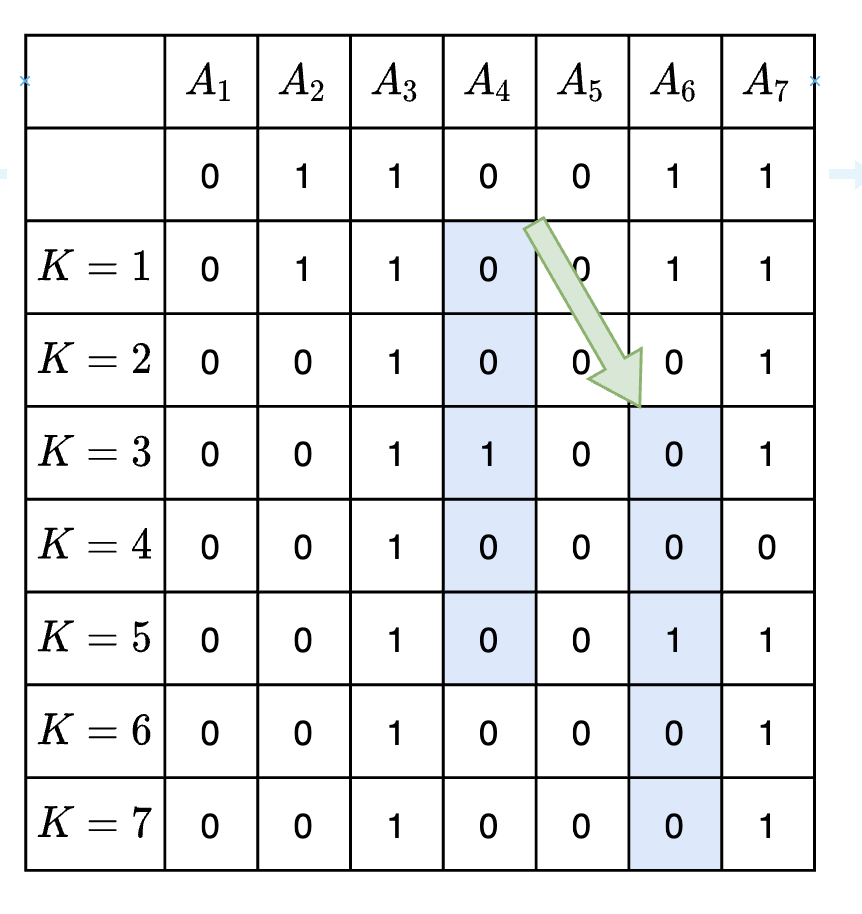
\includegraphics[scale=0.8]{20211128215156.png}

\begin{lstlisting}
// created on 25-10-17

const int N = 50010;

void solve(int id) {
	int n;
	cin >> n;

	string a, b;
	cin >> a >> b;

	a = "0" + a;

	bitset<N> k1, k0;
	for (int i = 0; i < n; i ++ ) k1[i] = 1;
	
	bitset<N> cmpb{b};
	vector<bitset<N>> cmpa(n + 1);
	vi pos(4 * n, -1);
	vi sa(n + 1);

	for (int i = 1; i <= n; i ++ ) {
		sa[i] = (a[i] - '0' ? 1 : -1);
		sa[i] += sa[i - 1];
	}

	int nw = 0;
	pos[2 * n] = 0;
	for (int i = 1; i <= n; i ++ ) {
		if (a[i] == '0') nw --;
		else nw ++;

		if (pos[nw + 2 * n] == -1) {
			if (sa[i] > 0) {
				cmpa[i] |= k1;
			} 
		} else {
			int j = pos[nw + 2 * n];
			if (sa[i] - sa[j + 1] > 0) {
				cmpa[i] |= (k1 >> (n - (i - j - 1)));
				cmpa[i] |= ((cmpa[j] << (i - j)) & k1);
			} else {
				cmpa[i] |= ((cmpa[j] << (i - j)) & k1);
			}
		}

		// cerr << i << " " << nw << "\n" << cmpa[i] << endl;

		pos[nw + 2 * n] = i;
	}

	bitset<N> ans = k1;
	for (int i = 1; i <= n; i ++ ) {
		if (cmpb[n - i] == 1) {
			cmpa[i] ^= k1;
		} else {
			cmpa[i] ^= k0;
		}
		ans &= (~cmpa[i]);
	}

	for (int i = 0; i < n; i ++ ) {
		cout << ans[i];
	}
	cout << endl;

	return;
}

signed main() {
	ios::sync_with_stdio(false);
	cin.tie(0);
	cout.tie(0);

	int _ = 1;
	cin >> _;

	rep(i, 1, _ + 1) {
		solve(i);
	}

	return 0;
}
\end{lstlisting}

\subsection{高精度}
\begin{lstlisting}
// created on 25-1-18

constexpr int N = 1000;

struct BigInt {
    int a[N];
    BigInt(int x = 0) : a{} {
        for (int i = 0; x; i++) {
            a[i] = x % 10;
            x /= 10;
        }
    }
    BigInt &operator*=(int x) {
        for (int i = 0; i < N; i++) {
            a[i] *= x;
        }
        for (int i = 0; i < N - 1; i++) {
            a[i + 1] += a[i] / 10;
            a[i] %= 10;
        }
        return *this;
    }
    BigInt &operator/=(int x) {
        for (int i = N - 1; i >= 0; i--) {
            if (i) {
                a[i - 1] += a[i] % x * 10;
            }
            a[i] /= x;
        }
        return *this;
    }
    BigInt &operator+=(const BigInt &x) {
        for (int i = 0; i < N; i++) {
            a[i] += x.a[i];
            if (a[i] >= 10) {
                a[i + 1] += 1;
                a[i] -= 10;
            }
        }
        return *this;
    }
};

std::ostream &operator<<(std::ostream &o, const BigInt &a) {
    int t = N - 1;
    while (a.a[t] == 0) {
        t--;
    }
    for (int i = t; i >= 0; i--) {
        o << a.a[i];
    }
    return o;
}
\end{lstlisting}
\newpage

\fancyhead[L]{字符串算法}
\section{字符串算法}
\subsection{KMP}

\subsubsection{KMP}

\noindent 应用:
\begin{enumerate}
\item 在字符串中寻找子串。
\item 最小周期:字符串长度 - f[字符串长度], 
形如 acaca 中 ac 是一个合法周期。
\item 最小循环节:区别于周期,当字符串长度$(n\%(n-f[n])==0)$时,等于最小周期,
否则为 n。形如 acac 中 ac 和 acac 是循环节, 而 aca 不是。
\end{enumerate}

\begin{lstlisting}
// created on 24-8-23

// kmp 原函数
typedef vector<int> vi;

vi kmp(const string s) {
	const int n = s.size();
	vi f(n + 1);
	for (int i = 1,j = 0;i < n;i++) {
		while (j and s[i] != s[j]) j = f[j];
		j += (s[i] == s[j]);
		f[i + 1] = j;
	}
	return f;
}
// 匹配字符串
string s = "ababab", t = "ab";
auto next = kmp(t);
for (int i = 0,j = 0;i < s.size();i++) {
    while (j and s[i] != t[j]) j = next[j];
    if (t[j] == s[i]) j++;
    if (j == t.size()) {
        cout << i << endl;
        j = next[j];
    }
}
\end{lstlisting}

\subsubsection{EXKMP}

\begin{lstlisting}
// created on 24-8-23

#define rep(i,a,n) for(int i=a;i<n;i++)
#define SZ(x) ((int)(x).size())
typedef vector<int> vi;

vi zFunction(const string& S) {
	vi z(SZ(S));
	int l=-1,r=-1;
	rep(i,1,SZ(S)) {
		z[i]=(i>=r?0:min(r-i,z[i-l]));
		while (i+z[i]<SZ(S)&&S[i+z[i]]==S[z[i]]) {
			z[i]++;
		}
		if (i+z[i]>r) {
			l=i,r=i+z[i];
		}
	}
	return z;
}
\end{lstlisting} 

\subsubsection{KMP 自动机}

\noindent 除此之外 KMP 还有一种比较特殊的用法, 
KMP 自动机, 像是单字符串的 AC 自动机。

\begin{lstlisting}
// created on 24-9-12

// CF 1721E
// 给定字符串 S,以及 Q 个字符串 Ti,求把 S 分别与每个 Ti 拼接后
// 最靠右的 |Ti| 个前缀的最长 border 长度, 询问分别独立。
// |S|<=1E6, Q<=1E5, |Ti|<=10

// O(26n) 的时间复杂度增加模板串长度
string s,t;
int n,q;
signed main(){
    cin>>s;
    s=" "+s;
    int n=s.size()-1;
    vector<array<int,26>> ch(n+20);
    vector<int> fail(n+20);
    for (int i=0;i<=n;i++) {
        if (i>1) fail[i]=ch[fail[i-1]][s[i]-'a'];
        if (i<n) {
            for (int j=0;j<26;j++) {
                if (s[i+1]-'a'==j) ch[i][j]=i+1;
                else ch[i][j]=ch[fail[i]][j];
            }
        }
    }
    int q;
    cin>>q;
    s+=string(10,'*');
    rep(tc,1,q+1) {
        cin>>t;
        int m=(t).size();
        for (int i=n+1;i<=n+m;i++) s[i]=t[i-n-1];
        for (int i=n;i<=n+m;i++) {
            if (i>1) fail[i]=ch[fail[i-1]][s[i]-'a'];
            if (i<n+m) {
                for (int j=0;j<26;j++) {
                    if (s[i+1]-'a'==j) ch[i][j]=i+1;
                    else ch[i][j]=ch[fail[i]][j];
                }
            }
            if (i>n) cout<<fail[i]<<" ";
        }
        cout<<endl;
    }
}
\end{lstlisting}

\subsection{字符串哈希}

\begin{lstlisting}
// created on 25-1-18

#define rep(i,a,n) for(int i=a;i<n;i++)
#define SZ(s) ((int)s.size())
typedef long long ll;
typedef uint64_t ull;

struct H {
    ull x; H(ull x=0) : x(x) {}
    H operator+(H o) { return x + o.x + (x + o.x < x); }
    H operator-(H o) { return *this + ~o.x; }
    H operator*(H o) { auto m = (__uint128_t)x * o.x;
        return H((ull)m) + (ull)(m >> 64); }
    ull get() const { return x + !~x; }
    bool operator==(H o) const { return get() == o.get(); }
    bool operator<(H o) const { return get() < o.get(); }
};
// (order ~ 3e9; random also ok)
static const H C = (ll)1e11+3;

struct HashInterval {
    vector<H> ha,pw;
    HashInterval(string& str):ha(SZ(str)+1),pw(ha) {
        pw[0]=1;
        rep(i,0,SZ(str))
            ha[i+1]=ha[i]*C+str[i],
            pw[i+1]=pw[i]*C;
    }
    H getHash(int a,int b) { // hash [a, b)
        return ha[b]-ha[a]*pw[b-a];
    }
};
// abcd
// get(2,4) * pw[2] + get(0,2) == cdab
// get(0,2) * pw[2] + get(2,4) == abcd
vector<H> getHashes(string& str,int length) {
    if (SZ(str)<length) return {};
    H h=0,pw=1;
    rep(i,0,length) {
        h=h*C+str[i],pw=pw*C;    
    }
    vector<H> ret={h};
    rep(i,length,SZ(str)) {
        ret.push_back(h=h*C+str[i]-pw*str[i-length]);
    }
    return ret;
}
H hashString(string& s){
    H h{}; 
    for(char c:s) h=h*C+c;return h;
}
signed main() {
    string s="abcabc",t="abc";
    HashInterval Q(s),P(t);
    cout<<Q.getHash(0,3).x<<" ";
    cout<<P.getHash(0,3).x<<endl;
}
\end{lstlisting}

\subsection{Manacher}

\noindent 其实 manacher 的用法也可以很灵活,
可以修改求的回文字符串的定义,从而求一些别的东西,比如求中心对称之类的东西

\begin{lstlisting}
// created on 25-5-12

vector<int> manacher(string a) {
    vi t{-1};
    for (auto c:a) {
        t.pb(c);
        t.pb(-1);
    }
    int n=t.size();
    vector<int> r(n);
    for (int i=0,j=0;i<n;i++) {
        if (2*j-i>=0&&j+r[j]>i) {
            r[i]=min(r[2*j-i],j+r[j]-i);
        } else {
        	r[i]=1;
        }
        while (i-r[i]>=0&&i+r[i]<n&&(t[i-r[i]]==t[i+r[i]])) {
            r[i]+=1;
        }
        if (i+r[i]>j+r[j]) {
            j=i;
        }
    }
    return r;
}
\end{lstlisting}

\subsection{Trie}

\begin{lstlisting}
// created on 2024-8-23

struct Trie{
    const int N=1e6+10;
    int nex[N][26],cnt;
    bool ok[N];
    void insert(string s) {
        int p=0; 
        for (int i=0;i<SZ(s);i++) {
            int c=s[i]-'a';
            if (!nex[p][c]) nex[p][c]=++cnt;
            p=nex[p][c];
        }
        ok[p]=1;
    }
    bool find(string s) {
        int p=0; 
        for (int i=0;i<SZ(s);i++) {
            int c=s[i]-'a';
            if (!nex[p][c]) return 0;
            p=nex[p][c];
        }
        return ok[p];
    }
}trie;
\end{lstlisting}

\noindent 可持久化 01 Trie 树:
给你长度为 $n$ 的数组 $a$, 以及 $q$ 次询问, 询问参数 $l,r,x$, 
$a$ 数组区间 $[l,r]$ 范围内, 最大的 $a_i \bigoplus x$ 是多少。

\begin{lstlisting}
// created on 25-3-27

const int N=200010;
int n,m,idx,cnt;
int rt[N],ch[N*33][2],siz[N*33];

void insert(int v){
    rt[++idx]=++cnt; //新根开点
    int x=rt[idx-1]; //旧版
    int y=rt[idx];   //新版
    for(int i=31;i>=0;i--){
        int j=v>>i&1;
        ch[y][!j]=ch[x][!j]; //异位继承
        ch[y][j]=++cnt;      //新位开点
        x=ch[x][j]; 
        y=ch[y][j]; 
        siz[y]=siz[x]+1;     //新位多1
    }
}
int query(int x,int y,int v){
    int ans=0;
    for(int i=31;i>=0;i--){
        int j=v>>i&1;
        if(siz[ch[y][!j]]>siz[ch[x][!j]]) {
            x=ch[x][!j];
            y=ch[y][!j];
            ans+=(1<<i);
        }
        else {
            x=ch[x][j];
            y=ch[y][j];
        }
    }
    return ans;
}
void clear() {
    for (int i=0;i<idx+10;i++) rt[i]=0;
    for (int i=0;i<cnt+10;i++) ch[i][0]=ch[i][1]=siz[i]=0;
    idx=cnt=0;
}
int main(){
    std::ios::sync_with_stdio(0);
    std::cin.tie(0);
    int t;
    cin>>t;
    while (t--) {
        clear();
        cin>>n>>m;
        int s=0;
        for (int i=1;i<=n;i++) {
            int x;
            cin>>x;
            insert(x);
        }
        while (m--) {
            int l,r,x;
            cin>>l>>r>>x;
            cout<<query(rt[l-1],rt[r],x)<<endl;
        }
    }
}
\end{lstlisting}

\subsection{AC 自动机}

\begin{lstlisting}
// created on 24-8-23

const int N=1e6+10;
struct ACAutoMaton {
    const int ALPHABET=26;
    ll ch[N][ALPHABET],link[N];
    ll tot,rt;
    ll cnt[N];
    void init() {
        tot=rt=0;
        memset(ch,0,sizeof ch);
        memset(link,0,sizeof link);
        memset(cnt,0,sizeof cnt);
    }
    void add(const string s,int id) {
        if (!rt) rt=++tot;
        int p=rt;
        for (auto c : s) {
            int x=(c-'a');
            p=ch[p][x]=(ch[p][x]?ch[p][x]:++tot);
        }
        cnt[p]++;
    }
    void build() {
        queue<int> q;
        for (int i=0;i<ALPHABET;i++) {
            if (ch[1][i]) {
                link[ch[1][i]]=1;
                q.push(ch[1][i]);
            } else ch[1][i]=1;
        }
        while (!q.empty()) {
            int x=q.front();
            q.pop();
            for (int i=0;i<ALPHABET;i++) {
                int y=ch[x][i];
                if (y) {
                    link[y]=ch[link[x]][i];
                    q.push(y);
                } else ch[x][i]=ch[link[x]][i];
            }
        }
    }
};
\end{lstlisting}

\noindent 结合二进制分组算法的ACAM,以 logn 时间复杂度为代价做到在线插入。

\begin{lstlisting}
// created on 24-8-23

// 其中包括 AC 自动机合并
// 其实就是 把 AC 自动机的 trie 树部分给合并
// 然后再把 link 在 build 一遍

struct AhoCorasick {
    static constexpr int ALPHABET = 26;
    int tire[N][ALPHABET],next[N][ALPHABET],link[N];
    int rt[N],size[N],top,tot;
    int ed[N],cnt[N];
    void build(int root) {
        queue<int> q;
        for (int i=0;i<ALPHABET;i++) {
            if(tire[root][i]) {
                link[next[root][i]=tire[root][i]]=root;
                q.push(next[root][i]);
            }
            else {
                next[root][i]=root;
            }
        }
        while (q.size()) {
            int top=q.front();
            q.pop();
            for (int i=0;i<ALPHABET;i++) {
                if (tire[top][i]) {
                    next[top][i]=tire[top][i];
                    link[next[top][i]]=next[link[top]][i];
                    q.push(next[top][i]);
                }
                else next[top][i]=next[link[top]][i];
            }
            cnt[top]=ed[top]+cnt[link[top]];
        }
    }
    int merge(int a,int b) {
        if (!a||!b) return a+b;
        ed[a]+=ed[b];
        for (int i=0;i<ALPHABET;i++)
        tire[a][i]=merge(tire[a][i],tire[b][i]);
        return a;
    }
    void add(string a,int val) {
        rt[++top]=++tot;
        size[top]=1;
        int now=rt[top];
        for (auto c : a){
            if(!tire[now][c-'a']) tire[now][c-'a']=++tot;
            now=tire[now][c-'a'];
        }
        ed[now]+=val;
        while (size[top]==size[top-1]){
            --top;
            rt[top]=merge(rt[top],rt[top+1]);
            size[top]+=size[top+1];
        }
        build(rt[top]);
    }
    int ask(string a) {
        int res=0;
        for (int i=1;i<=top;i++) {
            int now=rt[i];
            for (auto c : a) {
                now=next[now][c-'a'];
                res+=cnt[now];
            }
        }
        return res;
    }
};
\end{lstlisting}

\subsection{后缀数组}

\begin{lstlisting}
// created on 24-8-23

struct SuffixArray {
    int n;
    vector<int> sa,rk,lc;
    SuffixArray(const string &s) {
        n=s.length();
        sa.resize(n);
        lc.resize(n-1);
        rk.resize(n);
        iota(sa.begin(),sa.end(),0);
        sort(sa.begin(),sa.end(),[&](int a,int b) {
            return s[a]<s[b];
        });
        rk[sa[0]]=0;
        for (int i=1;i<n;++i) {
            rk[sa[i]]=rk[sa[i-1]]+(s[sa[i]]!=s[sa[i-1]]);
        }
        int k=1;
        vector<int> tmp,cnt(n);
        tmp.reserve(n);
        while (rk[sa[n-1]]<n-1) {
            tmp.clear();
            for (int i=0;i<k;++i)
            tmp.push_back(n-k+i);
            for (auto i : sa) {
                if (i>=k) {
                    tmp.push_back(i - k);
                }
            }
            fill(cnt.begin(),cnt.end(),0);
            for (int i=0;i<n;++i) ++cnt[rk[i]];
            for (int i=1;i<n;++i) cnt[i]+=cnt[i-1];
            for (int i=n-1;i>=0;--i) {
                sa[--cnt[rk[tmp[i]]]]=tmp[i];
            }
            swap(rk,tmp);
            rk[sa[0]]=0;
            for (int i=1;i<n;++i) {
                rk[sa[i]]=rk[sa[i-1]]
                +(tmp[sa[i-1]]<tmp[sa[i]]||sa[i-1]+k==n
                ||tmp[sa[i-1]+k]<tmp[sa[i]+k]);
            }
            k*=2;
        }
        for (int i=0,j=0;i<n;++i) {
            if (rk[i]==0) {
                j=0;
                continue;
            }
            for (j-=j>0;i+j<n&&
            sa[rk[i]-1]+j<n&&s[i+j]==s[sa[rk[i]-1]+j];) {
                ++j;
            }
            lc[rk[i]-1]=j;
        }
    }
};
\end{lstlisting}

\subsection{后缀自动机}

\begin{lstlisting}
// created on 24-8-23

//must #define int long long if you use the self_test
struct SAM {
    static const int MAXN=1000010,MAXS=28;
    int tot=1,last=1;
    int link[MAXN<<1],ch[MAXN<<1][MAXS];
    int len[MAXN<<1],endpos[MAXN<<1];
    void clear() {
        for (int i=0;i<=tot;i++) {
            link[i]=len[i]=endpos[i]=0;
            for (int k=0;k<MAXS;k++) {
                ch[i][k]=0;
            }
        }
        tot=1;last=1;
    }
    // extend a char,usual as [1-26]
    void extend(int w) {
        int p=++tot,x=last,r,q;
        endpos[p]=1;
        for (len[last=p]=len[x]+1;
        x&&!ch[x][w];x=link[x]) {
            ch[x][w]=p;
        }
        if (!x) link[p]=1;
        else if (len[x]+1==len[q=ch[x][w]]) link[p]=q;
        else {
            link[r=++tot]=link[q];
            memcpy(ch[r],ch[q],sizeof ch[r]);
            len[r]=len[x]+1;
            link[p]=link[q]=r;
            for (;x&&ch[x][w]==q;x=link[x]) {
                ch[x][w]=r;
            }
        }
    }
    // attention! memory of vector
    vector<int> p[MAXN<<1];
    void dfs(int u) {
        int v;
        for (int i=0;i<p[u].size();i++) {
            v=p[u][i];
            dfs(v);
            endpos[u]+=endpos[v];
        }
    }
    void get_endpos() {
        for (int i=1;i<=tot;i++) p[i].clear();
        for (int i=2;i<=tot;i++) {
            p[link[i]].push_back(i);
        }
        dfs(1);
        for (int i=1;i<=tot;i++) p[i].clear();
    }
    // test template is already and right
    // self_test will clear predate
    static const int STC = 998244353;
    void self_test() {
        clear();
        for (int i=1;i<=1000;i++) extend(i*i%26+1);
        int tmp=107*last+301*tot;
        for (int i=1;i<=tot;i++){
            tmp=(tmp*33+link[i]*101+len[i]*97) % STC;
            for (int k=1;k<MAXS;k++) {
                tmp=(tmp+k*ch[i][k])%STC;
            }
        }
        // stage1 
        // check build parent tree
        assert("stage 1" && tmp == 393281314);
        tmp=0; get_endpos();
        for (int i=1;i<=tot;i++) {
            tmp=(tmp*33+endpos[i])%STC;
        }
        // stage2
        // check endpos's mean
        // maybe errer if modify it.
        assert("stage 2" && tmp == 178417668);
        cout<<"Self Test Passed.";
        cout<<"Remember to delete this function's use.";
        cout<<endl;
        clear();
    }
    void debug_print() {
        for (int i=1;i<=tot;i++) {
            cout<<"node:"<<i<<" father:";
            cout<<link[i]<<" endpos:";
            cout<<endpos[i]<<"len:"<<len[i]<<endl;
        }
    }
    ll work() {
        // Do Something
        // Example luogu P3804
        ll ans=0;
        get_endpos();
        for (int i=1;i<=tot;i++) if (endpos[i]>=2) {
            ans=max(ans,(ll)endpos[i]*len[i]);
        }
        return ans;
    }
};
\end{lstlisting}

\subsection{回文自动机}

\begin{lstlisting}
// created on 24-8-23

// 1. 本质不同的回文串个数: idx - 2;
// 2. 回文子串出现次数;
// 对于一个字符串 s
// 它的本质不同回文子串个数最多只有 |s| 个。
// 那么回文树的时间复杂度为 O(|s|)。

struct PalindromeAutomaton {
    constexpr static int N=5e5+10;
    int tr[N][26],fail[N],len[N];
    int cntNodes,last;
    int cnt[N];
    string s;
    PalindromeAutomaton(string s) {
        memset(tr,0,sizeof tr);
        memset(fail,0,sizeof fail);
        len[0]=0,fail[0]=1;
        len[1]=-1,fail[1]=0;
        cntNodes=1;
        last=0;
        this->s=s;
    }
    void insert(char c,int i) {
        int u=get_fail(last,i);
        if (!tr[u][c-'a']) {
            int v=++cntNodes;
            fail[v]=tr[get_fail(fail[u],i)][c-'a'];
            tr[u][c-'a']=v;
            len[v]=len[u]+2;
            cnt[v]=cnt[fail[v]]+1;
        }
        last=tr[u][c-'a'];
    }
    int get_fail(int u,int i) {
        while (i-len[u]-1<=-1||s[i-len[u]-1]!=s[i]) {
            u=fail[u];
        }
        return u;
    }
};
\end{lstlisting}

\subsection{Other}

\subsubsection{最长公共子序列}

\begin{lstlisting}
// created on 24-8-23

// 求最长公共子序列 LCS
// n <= 1e5

const int INF=0x7fffffff;
int n,a[maxn],b[maxn],f[maxn],p[maxn];
int main(){
    cin >> n;
    for (int i=1;i<=n;i++){
        scanf("%d",&a[i]);
        p[a[i]]=i; //将第二个序列中的元素映射到第一个中
    }
    for (int i=1;i<=n;i++){
        scanf("%d",&b[i]);
        f[i]=INF;
    }
    int len=0;
    f[0]=0;
    for (int i=1;i<=n;i++){
        if (p[b[i]]>f[len]) f[++len]=p[b[i]];
        else {
            int l=0,r=len;
            while (l<r) {
                int mid=(l+r)>>1;
                if (f[mid]>p[b[i]]) r=mid;
                else l=mid+1;
            }
            f[l]=min(f[l],p[b[i]]);
        }
    }
    cout<<len<<"\n";
    return 0;
}
\end{lstlisting}
\newpage

\fancyhead[L]{常用数据结构}
\section{常用数据结构}

\subsection{并查集}

\begin{lstlisting}
// created on 25-1-18

struct DSU {
	vi f,siz;
	DSU() {}
	DSU(int n) {init(n);}
	void init(int n) {
		f.resize(n);
		siz.assign(n,1);
		iota(f.begin(),f.end(),0);
	}
	int find(int x) {
		while (x!=f[x]) {
			x=f[x]=f[f[x]];
		}
		return x;
	}
	bool merge(int x,int y) {
		x=find(x),y=find(y);
		if (x==y) return false;
		siz[x]+=siz[y];
		f[y]=x;
		return true;
	}
};
\end{lstlisting}

\subsection{ST 表}

\begin{lstlisting}
// created on 25-1-18

const int N=2e5+10,LOGN=19;
template<class T>
struct STTable {
    int n;
    T f[LOGN+1][N],g[LOGN+1][N];
    void init(vector<T> a) {
        n=SZ(a);
        assert(n<(1<<LOGN)&&n<N);
        rep(i,0,n) f[0][i]=g[0][i]=a[i];
        rep(j,1,LOGN) for (int i=0;i+(1<<j)-1<n;i++) {
            f[j][i]=min(f[j-1][i],f[j-1][i+(1<<(j-1))]);
            g[j][i]=max(g[j-1][i],g[j-1][i+(1<<(j-1))]);
        }
    }
    T querymin(int l,int r) {
        assert(l<=r);
        int len=31-__builtin_clz(r-l+1);
        return min(f[len][l],f[len][r-(1<<len)+1]);
    }
    T querymax(int l,int r) {
        assert(l<=r);
        int len=31-__builtin_clz(r-l+1);
        return max(g[len][l],g[len][r-(1<<len)+1]);
    }
};
STTable<int> f;
\end{lstlisting}

\subsection{树状数组}

\subsubsection{1D 树状数组}

\begin{lstlisting}
// created on 25-1-18

template <typename T>
struct Fenwick {
    int n;
    vector<T> a;
    Fenwick(int n_=0) {
        init(n_);
    }
    void init(int n_) {
        n=n_;
        a.assign(n,T{});
    }
    void add(int x,const T &v) { // 注意下标自动抬1
        for (int i=x+1;i<=n;i+=(i&-i)) {
            a[i-1]=a[i-1]+v;
        }
    }
    T sum(int x) { // 查值[1-(x-1)]
        T ans{};
        for (int i=x;i>0;i-=(i&-i)) {
            ans=ans+a[i-1];
        }
        return ans;
    }
};
\end{lstlisting}

\subsubsection{2D 树状数组}

\noindent 考虑到有时候出题人比较毒瘤,
赛时我可能铸币,可能连二维树状数组都写炸,所以这里贴另一套,但码风不统一就有点。

\begin{lstlisting}
// created on 25-1-18

struct FT {
    vector<ll> s;
    FT(int n):s(n) {}
    void update(int pos,ll dif) { // a[pos]+=dif
        for (;pos<sz(s);pos|=pos+1) s[pos]+=dif;
    }
    ll query(int pos) { // sum of values in [0, pos)
        ll res=0;
        for (;pos>0;pos&=pos-1) res+=s[pos-1];
        return res;
    }
    // min pos st sum of [0, pos] >= sum
    // Returns n if no sum is >= sum
    // or -1 if empty sum is.
    int lower_bound(ll sum) {
        if (sum<=0) return -1;
        int pos=0;
        for (int pw=1<<25;pw;pw>>=1) {
            if (pos+pw<=sz(s)&&s[pos+pw-1]<sum) {
                pos+=pw, sum-=s[pos-1];    
            }
        }
        return pos;
    }
};
struct FT2 {
    vector<vi> ys; vector<FT> ft;
    FT2(int limx) : ys(limx) {}
    void fakeUpdate(int x,int y) {
        for (;x<sz(ys);x|=x+1) ys[x].push_back(y);
    }
    void init() {
        for (vi& v : ys) {
            sort(all(v)), ft.emplace_back(sz(v));
        }
    }
    int ind(int x,int y) {
        return (lower_bound(all(ys[x]),y)-ys[x].begin()); 
    }
    void update(int x,int y,ll dif) {
        for (;x<sz(ys);x|=x+1) {
            ft[x].update(ind(x,y),dif);
        }
    }
    ll query(int x,int y) {
        ll sum=0;
        for (;x;x&=x-1) {
            sum+=ft[x-1].query(ind(x-1, y));
        }
        return sum;
    }
};
\end{lstlisting}

\subsection{线段树}

\subsubsection{基础线段树}

\begin{lstlisting}
// created on 24-8-23

const int N=1E5+10;
struct Node {
    int l,r;
    //
};
struct segtree {
    #define ls u<<1
    #define rs u<<1|1
    int n,a[N];
    Node tr[N*4];
    void up(Node &u,Node l,Node r) {
        //
        return;
    }
    void down(int u) {
        if (tr[u].xxx) {
            // lazy tag operation
        }
        return;
    }
    void build(int u,int l,int r) {
        //tr[u] initallize
        if (l==r) return;
        int mid=(l+r)/2;
        build(ls,l,mid);
        build(rs,mid+1,r);
        up(tr[u],tr[ls],tr[rs]);
    }
    void mdf(int u,int l,int r,int k) {
        if (l<=tr[u].l and tr[u].r<=r) {
            //
            return;
        }
        int mid=(tr[u].l+tr[u].r)/2;
        down(u);
        if (l<=mid) mdf(ls,l,r,k);
        if (r>mid) mdf(rs,l,r,k);
        up(tr[u],tr[ls],tr[rs]);
    }
    Node ask(int u,int l,int r) {
        if (l<=tr[u].l and tr[u].r<=r) return tr[u].xxx;
        int mid=(tr[u].l+tr[u].r)/2;
        down(u);
        Node t,a,b;
        //a = xxx, b = xxx;
        if (l<=mid) a=ask(ls,l,r);
        if (r>mid) b=ask(rs,l,r);
        up(t,a,b);
        return t;
    }
}s1;
\end{lstlisting}

\subsubsection{动态开点线段树}

\begin{lstlisting}
// created on 24-8-23

// CF915E
const int N=3E5*50;
struct segt {
    int root=0,tot=0;
    int ls[N],rs[N],sum[N],tag[N];
    segt() {
        init();
    }
    void init() {
        memset(tag,-1,sizeof tag);
    }
    void up(int u) {
        sum[u]=sum[ls[u]]+sum[rs[u]];
    }
    void down(int u,int nl,int nr) {
        if (tag[u]==-1) return;
        if (!ls[u]) ls[u]=++tot;
        if (!rs[u]) rs[u]=++tot;
        int mid=(nl+nr)/2;
        sum[ls[u]]=tag[u]*(mid-nl+1);
        sum[rs[u]]=tag[u]*(nr-mid);
        tag[ls[u]]=tag[rs[u]]=tag[u];
        tag[u]=-1;
    }
    void mdf(int &u,int nl,int nr,int l,int r,int k) {
        if (!u) u=++tot;
        if (l<=nl and nr<=r) {
            sum[u]=(nr-nl+1)*k;
            tag[u]=k;
            return;
        }
        int mid=(nl+nr)/2;
        down(u,nl,nr);
        if (l<=mid) mdf(ls[u],nl,mid,l,r,k);
        if (r>mid) mdf(rs[u],mid+1,nr,l,r,k);
        up(u);
    }
    int ask(int u,int nl,int nr,int l,int r) {
        if (l<=nl and nr<=r) return sum[u];
        int mid=(nl+nr)/2,ans=0;
        down(u,nl,nr);
        if (l<=mid) ans=ask(ls[u],nl,mid,l,r);
        if (r>mid) ans+=ask(rs[u],mid+1,nr,l,r);
        return ans;
    }
}s1; 
\end{lstlisting}

\subsubsection{权值线段树}

\begin{lstlisting}
// created on 24-8-23

// 给出n个数,以及q次询问(l,r),求区间[l,r]的mex。
const int N = 2e5 + 10;
struct op {//线段树维护区间最小值
    int val;
}seg[4 * N];//每个值的出现位置
//1-2段即为1,2出现位置最小的哪个
void pushup(int id) {
    seg[id].val = min(seg[id * 2].val, seg[id * 2 + 1].val);
}
//单点修改
void update(int id, int l, int r, int pos, int val){
    if (l == r) {
        seg[id].val = val;
        return;
    }
    else {
        int mid = (l + r) >> 1;
        if (mid >= pos) update(id * 2, l, mid, pos, val);
        else update(id * 2 + 1, mid + 1, r, pos, val);
        pushup(id);
    }
}
int query(int id, int l, int r, int val){
    if (l == r) return l;
    int mid = (l + r) >> 1;
    //区间l-mid的数出现的最小下标如果小于当前查询下标val
    //则递归到区间l-mid查询
    if (seg[2 * id].val < val) return query(2 * id, l, mid, val);
    //如果大等于val,则查询mid+1-r
    else return query(2 * id + 1, mid + 1, r, val);
}
update(1, 0, n + 1, a[i], i);//把a[i]的位置修改为i
query(1, 0, n + 1, t.first);//查询大等于t.first的mex
\end{lstlisting}

\subsubsection{基础主席树}

\begin{lstlisting}
// created on 24-8-23

const int maxn=1e5+100;
int a[maxn];
int rk[maxn];
int pos[maxn];
int root[maxn];
int cnt,m,n,T;
struct Segtree{
    struct Node{
        int L,R,val;
    }tree[maxn*500];
    void init() {
        memset(root,0,sizeof root);
        cnt=0;
    }
    /* 建T0空树 */
    int buildT0(int l, int r){
        int k=cnt++;
        tree[k].val=0;
        if (l==r) return k;
        int mid=l+r>>1;
        tree[k].L=buildT0(l, mid);
        tree[k].R=buildT0(mid+1,r);
        return k;
    }
    /* 上一个版本节点P,【ppos】+=del 返回新版本节点*/
    int update (int P,int l,int r,int ppos,int del){
        int k=cnt++;
        tree[k].val=tree[P].val+del;
        if (l==r) return k;
        int mid=l+r>>1;
        if (ppos<=mid){
            tree[k].L=update(tree[P].L,l,mid,ppos,del);
            tree[k].R=tree[P].R;
        }
        else {
            tree[k].L=tree[P].L;
            tree[k].R=update(tree[P].R,mid+1,r,ppos,del);
        }
        return k;
    }
    int query_kth(int lt,int rt,int l,int r,int k) {
        if (l==r) return a[rk[l]];
        int mid=l+r>>1;
        if (tree[tree[rt].L].val-tree[tree[lt].L].val>=k) {
            return query_kth(tree[lt].L,tree[rt].L,l,mid,k);
        }
        else {
            return query_kth(tree[lt].R,tree[rt].R,mid+1,r,
            k+tree[tree[lt].L].val-tree[tree[rt].L].val);
        }
    }
}tree;
bool cmp(int x,int y){return a[x]<a[y];}
int main() {
    scanf("%d",&T);
    while (T--) {
        scanf("%d%d",&n,&m);
        for (int i=1;i<=n;i++){
            scanf("%d",&a[i]);
            rk[i]=i;
        }
        tree.init();
        sort(rk+1,rk+1+n,cmp);
        for (int i1=1;i1<=n;i1++){
            pos[rk[i1]]=i1;
        }
        root[0]=tree.buildT0(1,n);
        for (int i1=1;i1<=n;i1++){
            root[i1]=tree.update(root[i1-1],1,n,pos[i1],1);
        }
        while (m--) {
            int l,r,k;scanf("%d%d%d",&l,&r,&k);
            printf("%d\n",tree.query_kth(root[l-1],root[r],1,n,k));
        }
    }
    return 0;
}
\end{lstlisting}

\subsubsection{线段树合并}

\noindent 线段树合并 + 权值线段树上二分模版题:

\begin{quote}
    永无乡包含 $n$ 座岛,编号从 $1$ 到 $n$ ,每座岛都有自己的独一无二的重要度,按照重要度可以将这 $n$ 座岛排名,名次用 $1$  到 $n$ 来表示。
    某些岛之间由巨大的桥连接,通过桥可以从一个岛到达另一个岛。
    如果从岛 $a$ 出发经过若干座(含 $0$ 座)桥可以 到达岛 $b$ ,则称岛 $a$ 和岛 $b$ 是连通的。
    \\

    现在有两种操作:

    B x y 表示在岛 $x$ 与岛 $y$ 之间修建一座新桥。
    \\
    
    Q x k 表示询问当前与岛 $x$ 连通的所有岛中第 $k$ 重要的是哪座岛,
    即所有与岛 $x$ 连通的岛中重要度排名第 $k$ 小的岛是哪座,请你输出那个岛的编号。        
\end{quote}


\begin{lstlisting}
// created on 25-5-1

int root[MAXN*50],tot=0;
int ls[MAXN*50],rs[MAXN*50],res[MAXN*50];
void up(int u) {
    res[u]=res[ls[u]]+res[rs[u]];
}
void mdf(int &u,int nl,int nr,int p,int k) {
    if (!u) u=++tot;
    if (nl==nr) {
        res[u]++;
        return;
    }
    int mid=(nl+nr)/2;
    if (p<=mid) mdf(ls[u],nl,mid,p,k);
    else mdf(rs[u],mid+1,nr,p,k);
    up(u);
}
int ask(int &u,int nl,int nr,int k) {
    // cerr<<"nw:"<<nl<<" "<<nr<<" "<<res[u]<<endl;
    if (nl==nr) return nl;
    int mid=(nl+nr)/2;
    if (res[ls[u]]>=k) 
        return ask(ls[u],nl,mid,k);
    if (res[rs[u]]>=k-res[ls[u]]) 
        return ask(rs[u],mid+1,nr,k-res[ls[u]]);
    return -1;
}
int merge(int x,int y,int l,int r) {
    if (!x or !y) return x+y;
    if (l==r) {
        res[x]+=res[y];
        return x;
    }
    int mid=(l+r)/2;
    ls[x]=merge(ls[x],ls[y],l,mid);
    rs[x]=merge(rs[x],rs[y],mid+1,r);
    up(x);
    return x;
}
int f[MAXN];
int find(int x) {
    while (x!=f[x]) {
        x=f[x]=f[f[x]];
    }
    return x;
} 
int p[MAXN];
int n,m,q;
bool QAQmerge(int x,int y) {
    x=find(x);
    y=find(y);
    if (x==y) return false;
    f[y]=x;
    merge(root[x],root[y],1,n);
    return true;
}

signed main(){
    // freopen("qwq.in","r",stdin);
    // freopen("qwq.out","w",stdout);

    ios::sync_with_stdio(false);
    cin.tie(nullptr);
    cout.tie(nullptr);

    cin>>n>>m;
    map<int,int> pos;
    rep(i,1,n+1) {
        cin>>p[i],f[i]=i;
        root[i]=++tot;
        mdf(root[i],1,n,p[i],1);
        pos[p[i]]=i;
        // cerr<<i<<" "<<p[i]<<endl;
    }
    rep(i,1,m+1) {
        int u,v;
        cin>>u>>v;
        QAQmerge(u,v);
    }
    cin>>q;
    rep(i,1,q+1) {
        char op;
        int x,y;
        cin>>op>>x>>y;
        if (op=='Q') {
            x=find(x);
            int ret=ask(root[x],1,n,y);
            if (ret!=-1) cout<<pos[ret]<<endl;
            else cout<<-1<<endl;
        }
        else {
            QAQmerge(x,y);
        }
    }
}
\end{lstlisting}

\subsubsection{吉司机线段树}

\noindent 维护区间最值和区间历史最值的线段树。
核心还是维护区间最大值和区间次大值,与势能相关,时间复杂度一般为 \(O(nlogn)\)。

\begin{itemize}
\item
    区间最值操作

    给定一个操作 \(l,r,k\),对于 \(i \in [l,r]\),将 \(a_i\) 变成
    \(min(a_i,k)\)。
\end{itemize}

\noindent 均摊时间复杂度为 \(O(nlogn)\)。

\begin{lstlisting}
// created on 24-9-1

// HDU 5306
#define ls u<<1
#define rs u<<1|1

struct Node {
	int l,r;
	int mx,smx,cnt,res;
	int tag;
}tr[MAXN*4];
int a[MAXN];
int n,m;
void up(Node &u,Node l,Node r) {
	u.res=l.res+r.res;
	u.mx=max(l.mx,r.mx),u.smx=max(l.smx,r.smx);
	u.cnt=0;
	if (u.mx==l.mx) u.cnt+=l.cnt;
	else u.smx=max(u.smx,l.mx);
	if (u.mx==r.mx) u.cnt+=r.cnt;
	else u.smx=max(u.smx,r.mx);
}
void build(int u,int l,int r) {
	tr[u]={l,r};
	tr[u].tag=-1;
	if (l==r) {
		tr[u].mx=tr[u].res=a[l];
		tr[u].smx=-1,tr[u].cnt=1;
		return;
	}
	int mid=(l+r)/2;
	build(ls,l,mid);
	build(rs,mid+1,r);
	up(tr[u],tr[ls],tr[rs]);
}
void update(int u,int k) {
	if (k<tr[u].mx) {
		tr[u].res+=(1ll*k-tr[u].mx)*tr[u].cnt;
		tr[u].mx=tr[u].tag=k;
	}
}
void down(int u) {
	if (tr[u].tag>=0) {
		update(ls,tr[u].tag);
		update(rs,tr[u].tag);
		tr[u].tag=-1;
	} 
}
void mdf(int u,int l,int r,int k) {
	if (k>=tr[u].mx) return;
	if (l<=tr[u].l and tr[u].r<=r and k>tr[u].smx) {
		update(u,k);
		return;
	}
	down(u);
	int mid=(tr[u].l+tr[u].r)/2;
	if (l<=mid) mdf(ls,l,r,k);
	if (r>mid) mdf(rs,l,r,k);
	up(tr[u],tr[ls],tr[rs]);
}
Node ask(int u,int l,int r) {
	if (l<=tr[u].l and tr[u].r<=r) {
		return tr[u];
	}
	int mid=(tr[u].l+tr[u].r)/2;
	down(u);
	Node t;
	if (l<=mid and r>mid) {
		up(t,ask(ls,l,r),ask(rs,l,r));
		return t;
	}
	if (l<=mid) t=ask(ls,l,r);
	if (r>mid) t=ask(rs,l,r);
	return t;
}    
\end{lstlisting}

\begin{itemize}
\item
    区间加减操作

    标记换成二元组 \((add,v)\),表示将当前节点维护的区间先加上 \(add\) 再与
    \(v\) 取最小值。

    合并标记时,比如区间加 \(x\),当前节点的懒标记变为
    \((add+x,v+x)\),然后标记向下传递的时候,儿子 \(ch\) 的标记更新为
    \((add_{ch}+add_x,min(v_{ch}+add_x,v_x))\)。
    
    当然还有更加 \(edu\) 的方面,跟上面很像,我们把线段树上面的元素分成了
    \textbf{最大值和非最大值} 两类,然后建立的懒标记只会打在
    \(mx2 < v < mx1\)
    的节点上,然后修改对于这种情况就直接修改,不然就递归下去,然后区间加操作对于这两类值都生效。
\end{itemize}

\begin{lstlisting}
// created on 24-9-1

// BZOJ 4695
// 给一个区间 [L,R] 加上一个数 x 
// 把一个区间 [L,R] 里小于 x 的数变成 x 
// 把一个区间 [L,R] 里大于 x 的数变成 x 
// 求区间 [L,R] 的和
// 求区间 [L,R] 的最大值
// 求区间 [L,R] 的最小值

template<typename T>
void chmax(T &x,T y) {
    if (x<y) x=y;
}
template<typename T>
void chmin(T &x,T y) {
    if (x>y) x=y;
}

const ll MAXN=5e5+10,inf=0x3f3f3f3f3f3f3f3fll;
ll a[MAXN];
ll n,q;
struct Node {
    ll l,r;
    ll sum,mx1,mx2,mn1,mn2;
    ll mxcnt,mncnt;
    ll tagmx,tagmn,tags;
};
struct segtree {
    Node tr[MAXN*4];
    #define ls u*2
    #define rs u*2+1
    void up(Node &u,Node l,Node r) {
        u.sum=l.sum+r.sum;
        u.mx1=max(l.mx1,r.mx1);
        u.mx2=-inf;
        if (l.mx1<u.mx1) chmax(u.mx2,l.mx1);
        if (l.mx2<u.mx1) chmax(u.mx2,l.mx2);
        if (r.mx1<u.mx1) chmax(u.mx2,r.mx1);
        if (r.mx2<u.mx1) chmax(u.mx2,r.mx2);
        u.mxcnt=0;
        if (l.mx1==u.mx1) u.mxcnt+=l.mxcnt;
        if (r.mx1==u.mx1) u.mxcnt+=r.mxcnt;
        u.mn1=min(l.mn1,r.mn1);
        u.mn2=inf;
        if (l.mn1>u.mn1) chmin(u.mn2,l.mn1);
        if (l.mn2>u.mn1) chmin(u.mn2,l.mn2);
        if (r.mn1>u.mn1) chmin(u.mn2,r.mn1);
        if (r.mn2>u.mn1) chmin(u.mn2,r.mn2);
        u.mncnt=0;
        if (l.mn1==u.mn1) u.mncnt+=l.mncnt;
        if (r.mn1==u.mn1) u.mncnt+=r.mncnt;
    }
    void pushs(ll u,ll tag) {
        tr[u].sum+=tag*(tr[u].r-tr[u].l+1);
        if (tr[u].mx1!=-inf) tr[u].mx1+=tag;
        if (tr[u].mx2!=-inf) tr[u].mx2+=tag;
        if (tr[u].mn1!=inf) tr[u].mn1+=tag;
        if (tr[u].mn2!=inf) tr[u].mn2+=tag;
        tr[u].tags+=tag;
        if (tr[u].tagmx!=-inf) tr[u].tagmx+=tag;
        if (tr[u].tagmn!=inf) tr[u].tagmn+=tag;
    }
    void pushmx(ll u,ll tag) { // max(a[i],tag) 修改 min1
        if (tr[u].mn1>tag) return;
        tr[u].sum+=(tag-tr[u].mn1)*tr[u].mncnt;
        // 下面三行直接修改最小值。。。
        // 次大值等于最最值,应该被最大值标记作用
        if (tr[u].mx2==tr[u].mn1) tr[u].mx2=tag;
        if (tr[u].mx1==tr[u].mn1) tr[u].mx1=tag;
        tr[u].mn1=tag;
        // 维护非最小值的懒标记。。。
        chmax(tr[u].tagmx,tag);
        chmax(tr[u].tagmn,tag);
    }
    void pushmn(ll u,ll tag) { // min(a[i],tag) 修改 max1
            // 如果区间中最大值都小于就直接 return
        if (tr[u].mx1<tag) return;
        tr[u].sum+=(tag-tr[u].mx1)*tr[u].mxcnt;
        if (tr[u].mn2==tr[u].mx1) tr[u].mn2=tag;
        if (tr[u].mn1==tr[u].mx1) tr[u].mn1=tag;
        tr[u].mx1=tag;
        chmin(tr[u].tagmx,tag);
        chmin(tr[u].tagmn,tag);
    }
    void down(ll u) {
        if (tr[u].tags) {
            pushs(ls,tr[u].tags);
            pushs(rs,tr[u].tags);
            tr[u].tags=0;
        }
        if (tr[u].tagmx!=-inf) {
            pushmx(ls,tr[u].tagmx);
            pushmx(rs,tr[u].tagmx);
            tr[u].tagmx=-inf;
        }
        if (tr[u].tagmn!=inf) {
            pushmn(ls,tr[u].tagmn);
            pushmn(rs,tr[u].tagmn);
            tr[u].tagmn=inf;
        }
    }
    void build(ll u,ll l,ll r) {
        tr[u].l=l,tr[u].r=r;
        tr[u].tags=0;
        tr[u].tagmx=-inf;
        tr[u].tagmn=inf;
        if (l==r) {
            tr[u].sum=tr[u].mx1=tr[u].mn1=a[l];
            tr[u].mxcnt=tr[u].mncnt=1;
            tr[u].mx2=-inf;
            tr[u].mn2=inf;
            return;
        }
        ll mid=(l+r)/2;
        build(ls,l,mid);
        build(rs,mid+1,r);
        up(tr[u],tr[ls],tr[rs]);
    }
    void mdfs(ll u,ll l,ll r,ll k) {
        if (l<=tr[u].l and tr[u].r<=r) {
            pushs(u,k);
            return;
        }
        ll mid=(tr[u].l+tr[u].r)/2;
        down(u);
        if (l<=mid) mdfs(ls,l,r,k);
        if (r>mid) mdfs(rs,l,r,k);
        up(tr[u],tr[ls],tr[rs]);
    }
    void mdfmx(ll u,ll l,ll r,ll k) {
        if (tr[u].mn1>=k) return;
        if (l<=tr[u].l and tr[u].r<=r and tr[u].mn2>k) {
            // 只有 tr[u].mn1 受影响的情况
            // 修改 打标记
            pushmx(u,k);
            return;
        }
        ll mid=(tr[u].l+tr[u].r)/2;
        down(u);
        if (l<=mid) mdfmx(ls,l,r,k);
        if (r>mid) mdfmx(rs,l,r,k);
        up(tr[u],tr[ls],tr[rs]);
    }
    void mdfmn(ll u,ll l,ll r,ll k) {
        if (tr[u].mx1<=k) return;
        if (l<=tr[u].l and tr[u].r<=r and tr[u].mx2<k) {
            // 只有 tr[u].mx1 受影响的情况
            // 修改 打标记
            pushmn(u,k);
            return;
        }
        ll mid=(tr[u].l+tr[u].r)/2;
        down(u);
        if (l<=mid) mdfmn(ls,l,r,k);
        if (r>mid) mdfmn(rs,l,r,k);
        up(tr[u],tr[ls],tr[rs]);
    }
    ll asks(ll u,ll l,ll r) {
        if (l<=tr[u].l and tr[u].r<=r) 
            return tr[u].sum;
        ll mid=(tr[u].l+tr[u].r)/2;
        down(u);
        ll ans=0;
        if (l<=mid) ans+=asks(ls,l,r);
        if (r>mid) ans+=asks(rs,l,r);
        up(tr[u],tr[ls],tr[rs]);
        return ans;
    }
    ll askmx(ll u,ll l,ll r) {
        if (l<=tr[u].l and tr[u].r<=r) 
            return tr[u].mx1;
        ll mid=(tr[u].l+tr[u].r)/2;
        down(u);
        ll ans=-inf;
        if (l<=mid) chmax(ans,askmx(ls,l,r));
        if (r>mid) chmax(ans,askmx(rs,l,r));
        up(tr[u],tr[ls],tr[rs]);
        return ans;
    }
    ll askmn(ll u,ll l,ll r) {
        if (l<=tr[u].l and tr[u].r<=r) 
            return tr[u].mn1;
        ll mid=(tr[u].l+tr[u].r)/2;
        down(u);
        ll ans=inf;
        if (l<=mid) chmin(ans,askmn(ls,l,r));
        if (r>mid) chmin(ans,askmn(rs,l,r));
        up(tr[u],tr[ls],tr[rs]);
        return ans;
    }
    #undef ls
    #undef rs
}s1;
\end{lstlisting}

\begin{itemize}
\item 
    区间历史最值

    不难发现有了区间加减操作之后,我们的区间最值操作,在 \(mx2 < v < mx1\)
    的情况下,我们可以把 \(mx1\) 加上 \(k-mx1\),以实现相同的效果。
    
    而且有了区间加减之后,实现区间最值也可能只能用这种减的方式实现了QAQ。
    
    于是就有了下面的代码。
    
    \(mx1\) 区间最大值,\(mx2\) 区间严格次大值,\(hmx\)
    区间历史最大值,\(mxcnt\) 区间最大值出现次数,\(sum\) ...
    
    \(add1\) 区间最大值加减标记,\(add1\_\) 历史中最大的加减标记,\(add2\)
    区间非最大值加减标记,\(add2\_\) ...
    
    首先为什么要这样设置,\(add1 \ \& \ add2\)
    这种跟上面一样的思维,对最大值和非最大值分类讨论;然后就是
    \(add1\_ \ \& \ add2\_\) 就是为了更新历史最大值而存在的,每次
    \(down(u)\) 都会结算当前节点的懒标记,考虑到定义能更新该区间的数值就是
    \(mx1 + add1\_\) (也可以知道 \(add1\_\)
    不会为负数),更新完历史最大值之后就用 \(add1\) 把 \(mx1\) 设成当前的值。   
\end{itemize}

\begin{lstlisting}
// created on 24-9-1

void chmax(ll &x,ll y) {
    if (x<y) x=y;
}

const ll MAXN=5e5+10,inf=1e18;
ll a[MAXN];
int n,m;
struct Node {
    int l,r;
    ll mx1,mx2,hmx,mxcnt,sum;
    ll add1,add1_,add2,add2_;
};
struct segtree {
    Node tr[MAXN*4];
    #define ls u*2
    #define rs u*2+1
    void up(Node &u,Node l,Node r){
        u.sum=l.sum+r.sum;
        u.hmx=max(l.hmx,r.hmx);
        if (l.mx1==r.mx1) {
            u.mx1=l.mx1;
            u.mx2=max(l.mx2,r.mx2);
            u.mxcnt=l.mxcnt+r.mxcnt;
        }
        else if (l.mx1>r.mx1) {
            u.mx1=l.mx1;
            u.mx2=max(l.mx2,r.mx1);
            u.mxcnt=l.mxcnt;
        }
        else {
            u.mx1=r.mx1;
            u.mx2=max(l.mx1,r.mx2);
            u.mxcnt=r.mxcnt;
        }
    }
    void upd(ll u,ll k1,ll k1_,ll k2,ll k2_) {
        tr[u].sum+=tr[u].mxcnt*k1
        +(tr[u].r-tr[u].l+1-tr[u].mxcnt)*k2;
        chmax(tr[u].hmx,tr[u].mx1+k1_);
        chmax(tr[u].add1_,tr[u].add1+k1_);
        tr[u].mx1+=k1;
        tr[u].add1+=k1;
        chmax(tr[u].add2_,tr[u].add2+k2_);
        if (tr[u].mx2!=-inf) tr[u].mx2+=k2;
        tr[u].add2+=k2;
    }
    void down(ll u) {
        ll tmp=max(tr[ls].mx1,tr[rs].mx1);
        if (tr[ls].mx1==tmp) 
            upd(ls,tr[u].add1,tr[u].add1_,tr[u].add2,tr[u].add2_);
        else 
            upd(ls,tr[u].add2,tr[u].add2_,tr[u].add2,tr[u].add2_);
        if (tr[rs].mx1==tmp)
            upd(rs,tr[u].add1,tr[u].add1_,tr[u].add2,tr[u].add2_);
        else 
            upd(rs,tr[u].add2,tr[u].add2_,tr[u].add2,tr[u].add2_);
        tr[u].add1=tr[u].add1_=tr[u].add2=tr[u].add2_=0;
    }
    void build(ll u,ll l,ll r) {
        tr[u].l=l,tr[u].r=r;
        tr[u].add1=tr[u].add1_=tr[u].add2=tr[u].add2_=0;
        if (l==r) {
            tr[u].sum=tr[u].hmx=tr[u].mx1=a[l];
            tr[u].mxcnt=1;
            tr[u].mx2=-inf;
            return;
        }
        int mid=(l+r)/2;
        build(ls,l,mid);
        build(rs,mid+1,r);
        up(tr[u],tr[ls],tr[rs]);
    }
    void mdf1(int u,int l,int r,int k) {
        if (l<=tr[u].l and tr[u].r<=r) {
            upd(u,k,k,k,k);
            return;
        }
        down(u);
        int mid=(tr[u].l+tr[u].r)/2;
        if (l<=mid) mdf1(ls,l,r,k);
        if (r>mid) mdf1(rs,l,r,k);
        up(tr[u],tr[ls],tr[rs]);
    }
    void mdf2(int u,int l,int r,int k) {
        // cerr<<tr[u].l<<" "<<tr[u].r<<endl;
        if (k>=tr[u].mx1) return;
        if (l<=tr[u].l and tr[u].r<=r and k>tr[u].mx2) {
            upd(u,k-tr[u].mx1,k-tr[u].mx1,0,0);
            return;
        }
        down(u);
        int mid=(tr[u].l+tr[u].r)/2;
        if (l<=mid) mdf2(ls,l,r,k);
        if (r>mid) mdf2(rs,l,r,k);
        up(tr[u],tr[ls],tr[rs]);
    }
    Node ask(int u,int l,int r) {
        if (l<=tr[u].l and tr[u].r<=r) 
            return tr[u];
        int mid=(tr[u].l+tr[u].r)/2;
        down(u);
        Node t;
        if (l<=mid and r>mid) {
            up(t,ask(ls,l,r),ask(rs,l,r));
            return t;
        } 
        if (l<=mid) t=ask(ls,l,r);
        if (r>mid) t=ask(rs,l,r);
        return t;
    }
    #undef ls
    #undef rs
}s1;
\end{lstlisting}

\subsubsection{单点修改 + 区间最值}

\begin{lstlisting}
// created on 24-8-23

struct Segt {
    vector<int> w;
    int n;
    Segt(int n) : w(2 * n, (int)-2E9), n(n) {}
    void modify(int pos, int val) {
        for (w[pos += n] = val; pos > 1; pos /= 2) {
            w[pos / 2] = max(w[pos], w[pos ^ 1]);
        }
    }
    int ask(int l, int r) {
        int res = -2E9;
        for (l += n, r += n; l < r; l /= 2, r /= 2) {
            if (l % 2) res = max(res, w[l++]);
            if (r % 2) res = max(res, w[--r]);
        }
        return res;
    }
};   
\end{lstlisting}

\subsubsection{区间加法 + 区间乘法}

\begin{lstlisting}
// created on 24-8-23

template <class T> struct Segt_ {
    struct node {
        int l, r;
        T w, add, mul = 1; // 注意初始赋值
    };
    vector<T> w;
    vector<node> t;
    Segt_(int n) {
        w.resize(n + 1);
        t.resize((n << 2) + 1);
        build(1, n);
    }
    Segt_(vector<int> in) {
        int n = in.size() - 1;
        w.resize(n + 1);
        for (int i = 1; i <= n; i++) {
            w[i] = in[i];
        }
        t.resize((n << 2) + 1);
        build(1, n);
    }
    void pushdown(node &p, T add, T mul) { // 在此更新下递函数
        p.w = p.w * mul + (p.r - p.l + 1) * add;
        p.add = p.add * mul + add;
        p.mul *= mul;
    }
    void pushup(node &p, node &l, node &r) { // 在此更新上传函数
        p.w = l.w + r.w;
    }
    #define GL (k << 1)
    #define GR (k << 1 | 1)
    void pushdown(int k) { // 不需要动
        pushdown(t[GL], t[k].add, t[k].mul);
        pushdown(t[GR], t[k].add, t[k].mul);
        t[k].add = 0, t[k].mul = 1;
    }
    void pushup(int k) { // 不需要动
        pushup(t[k], t[GL], t[GR]);
    }
    void build(int l, int r, int k = 1) {
        if (l == r) {
            t[k] = {l, r, w[l]};
            return;
        }
    t[k] = {l, r};
        int mid = (l + r) / 2;
        build(l, mid, GL);
        build(mid + 1, r, GR);
        pushup(k);
    }
    void modify(int l, int r, T val, int k = 1) { // 区间修改
        if (l <= t[k].l && t[k].r <= r) {
            t[k].w += (t[k].r - t[k].l + 1) * val;
            t[k].add += val;
            return;
        }
        pushdown(k);
        int mid = (t[k].l + t[k].r) / 2;
        if (l <= mid) modify(l, r, val, GL);
        if (mid < r) modify(l, r, val, GR);
        pushup(k);
    }
    void modify2(int l, int r, T val, int k = 1) { // 区间修改
        if (l <= t[k].l && t[k].r <= r) {
            t[k].w *= val;
            t[k].add *= val;
            t[k].mul *= val;
            return;
        }
        pushdown(k);
        int mid = (t[k].l + t[k].r) / 2;
        if (l <= mid) modify2(l, r, val, GL);
        if (mid < r) modify2(l, r, val, GR);
        pushup(k);
    }
    T ask(int l, int r, int k = 1) { // 区间询问,不合并
        if (l <= t[k].l && t[k].r <= r) {
            return t[k].w;
        }
        pushdown(k);
        int mid = (t[k].l + t[k].r) / 2;
        T ans = 0;
        if (l <= mid) ans += ask(l, r, GL);
        if (mid < r) ans += ask(l, r, GR);
        return ans;
    }
    void debug(int k = 1) {
        cout << "[" << t[k].l << ", " << t[k].r << "]: ";
        cout << "w = " << t[k].w << ", ";
        cout << "add = " << t[k].add << ", ";
        cout << "mul = " << t[k].mul << ", ";
        cout << endl;
        if (t[k].l == t[k].r) return;
        debug(GL), debug(GR);
    }
};
\end{lstlisting}

\subsubsection{区间取模}

\noindent 原题需要进行“单点赋值+区间取模+区间求和”。该操作不需要懒标记。
\\

\noindent 需要额外维护一个区间最大值,当模数大于区间最大值时剪枝,否则进行单点取模。最劣的情况只需要 \(log x\) 次。

\begin{lstlisting}
// created on 24-8-23

// https://codeforces.com/contest/438/problem/D
void modifyMod(int l, int r, T val, int k = 1) {
    if (l <= t[k].l && t[k].r <= r) {
        if (t[k].rmq < val) return; // 重要剪枝
    }
    if (t[k].l == t[k].r) {
        t[k].w %= val;
        t[k].rmq %= val;
        return;
    }
    int mid = (t[k].l + t[k].r) / 2;
    if (l <= mid) modifyMod(l, r, val, GL);
    if (mid < r) modifyMod(l, r, val, GR);
    pushup(k);
}   
\end{lstlisting}

\subsubsection{区间异或修改 + 区间求和}

\begin{lstlisting}
// created on 24-8-24

// https://codeforces.com/contest/242/problem/E
struct Segt { // #define GL (k << 1) // #define GR (k << 1 | 1)
    struct node {
        int l, r;
        int w[N], lazy; // 注意这里为了方便计算,w 只需要存位
    };
    vector<int> base;
    vector<node> t;
    Segt(vector<int> in) : base(in) {
        int n = in.size() - 1;
        t.resize(n * 4 + 1);
        auto build = [&](auto self, int l, int r, int k = 1) {
            t[k] = {l, r}; // 前置赋值
            if (l == r) {
                for (int i = 0; i < N; i++) {
                    t[k].w[i] = base[l] >> i & 1;
                }
                return;
            }
            int mid = (l + r) / 2;
            self(self, l, mid, GL);
            self(self, mid + 1, r, GR);
            pushup(k);
        };
        build(build, 1, n);
    }
    void pushdown(node &p, int lazy) { /* 【在此更新下递函数】 */
        int len = p.r - p.l + 1;
        for (int i = 0; i < N; i++) {
            if (lazy >> i & 1) { // 即 p.w = (p.r - p.l + 1) - p.w;
                p.w[i] = len - p.w[i];
            }
        }
        p.lazy ^= lazy;
    }
    void pushdown(int k) { // 【不需要动】
        if (t[k].lazy == 0) return;
        pushdown(t[GL], t[k].lazy);
        pushdown(t[GR], t[k].lazy);
        t[k].lazy = 0;
    }
    void pushup(int k) {
        auto pushup = [&](node &p, node &l, node &r) { /* 【在此更新上传函数】
            */
            for (int i = 0; i < N; i++) {
                p.w[i] = l.w[i] + r.w[i]; // 即 p.w = l.w + r.w;
            }
        };
        pushup(t[k], t[GL], t[GR]);
    }
    void modify(int l, int r, int val, int k = 1) { // 区间修改
        if (l <= t[k].l && t[k].r <= r) {
            pushdown(t[k], val);
            return;
        }
        pushdown(k);
        int mid = (t[k].l + t[k].r) / 2;
        if (l <= mid) modify(l, r, val, GL);
        if (mid < r) modify(l, r, val, GR);
        pushup(k);
    }
    i64 ask(int l, int r, int k = 1) { // 区间求和
        if (l <= t[k].l && t[k].r <= r) {
            i64 ans = 0;
            for (int i = 0; i < N; i++) {
                ans += t[k].w[i] * (1LL << i);
            }
            return ans;
        }
        pushdown(k);
        int mid = (t[k].l + t[k].r) / 2;
        i64 ans = 0;
        if (l <= mid) ans += ask(l, r, GL);
        if (mid < r) ans += ask(l, r, GR);
        return ans;
    }
};
\end{lstlisting}

\subsubsection{拆位运算线段树}

\noindent 使用若干颗线段树维护每一位的值, 区间异或转变为区间翻转。

\begin{lstlisting}
// created on 24-8-24
template<class T> struct Segt_ { // GL 为 (k << 1),GR 为 (k << 1 | 1)
    struct node {
        int l, r;
        T w;
        bool lazy; // 注意懒标记用布尔型足以
    };
    vector<T> w;
    vector<node> t;
    Segt_() {}
    void init(vector<int> in) {
        int n = in.size() - 1;
        w.resize(n * 4 + 1);
        for (int i = 0; i <= n; i++) { 
            w[i] = in[i]; 
        }
        t.resize(n * 4 + 1);
        build(1, n);
    }
    void pushdown(node &p, bool lazy = 1) { // 【在此更新下递函数】
        p.w = (p.r - p.l + 1) - p.w;
        p.lazy ^= lazy;
    }
    void pushup(node &p, node &l, node &r) { // 【在此更新上传函数】
        p.w = l.w + r.w;
    }
    void pushdown(int k) { // 【不需要动】
        if (t[k].lazy == 0) return;
        pushdown(t[GL]), pushdown(t[GR]); // 注意这里不再需要传入第二个参数
        t[k].lazy = 0;
    }
void pushup(int k) { pushup(t[k], t[GL], t[GR]); } // 【不需要动】
    void build(int l, int r, int k = 1) {
        if (l == r) {
            t[k] = {l, r, w[l], 0}; // 注意懒标记初始为 0
            return;
        }
        t[k] = {l, r};
        int mid = (l + r) / 2;
        build(l, mid, GL);
        build(mid + 1, r, GR);
        pushup(k);
    }
    void reverse(int l, int r, int k = 1) { // 区间翻转
        if (l <= t[k].l && t[k].r <= r) {
            pushdown(t[k], 1);
            return;
        }
        pushdown(k);
        int mid = (t[k].l + t[k].r) / 2;
        if (l <= mid) reverse(l, r, GL);
        if (mid < r) reverse(l, r, GR);
        pushup(k);
    }
    T ask(int l, int r, int k = 1) { // 区间求和
        if (l <= t[k].l && t[k].r <= r) {
            return t[k].w;
        }
        pushdown(k);
        int mid = (t[k].l + t[k].r) / 2;
        T ans = 0;
        if (l <= mid) ans += ask(l, r, GL);
        if (mid < r) ans += ask(l, r, GR);
        return ans;
    }
};
signed main() {
    int n; 
    cin >> n;
    vector in(20, vector<int>(n + 1));
    Segt_<i64> segt[20]; // 拆位建线段树
    for (int i = 1, x; i <= n; i++) { 
        cin >> x;
        for (int bit = 0; bit < 20; bit++) {
            in[bit][i] = x >> bit & 1;
        }
    }
    for (int i = 0; i < 20; i++) {
        segt[i].init(in[i]);
    }
    int m, op;
    for (cin >> m; m; m--) { 
        cin >> op;
        if (op == 1) {
            int l, r; 
            i64 ans = 0; 
            cin >> l >> r;
            for (int i = 0; i < 20; i++) {
                ans += segt[i].ask(l, r) * (1LL << i);
            }
            cout << ans << "\n";
        } else {
            int l, r, val; 
            cin >> l >> r >> val;
            for (int i = 0; i < 20; i++) {
                if (val >> i & 1) { 
                    segt[i].reverse(l, r); 
                }
            }
        }
    }
}
\end{lstlisting}

\subsubsection{树上线段树}

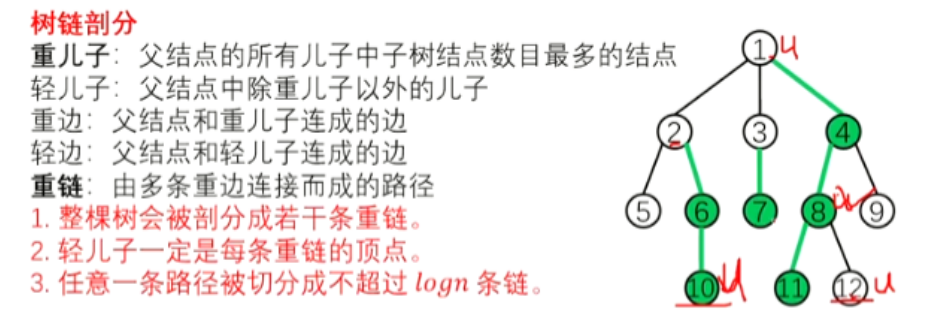
\includegraphics[scale=0.8]{线段树1.png}

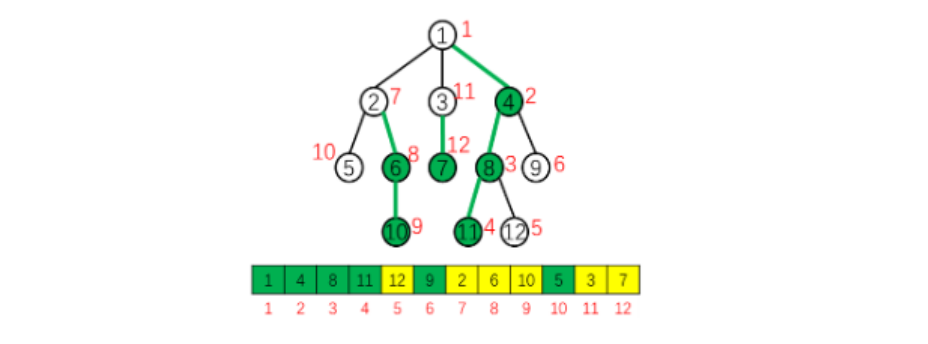
\includegraphics[scale=0.8]{线段树2.png}

\noindent 红色的数字是重新分配的编号, 我们区间修改使用这个编号。
\\

\noindent 树链剖分 + 区间查询维护模版:

\begin{quote}
如题,已知一棵包含 个结点的树,每个节点上包含一个数值,需要支持以下操作:
\begin{itemize}
    \item 1 x y z,表示将树从 到 结点最短路径上所有节点的值都加上。
    \item 2 x y,表示求树从 到 结点最短路径上所有节点的值之和。
    \item 3 x z,表示将以 为根节点的子树内所有节点值都加上。
    \item 4 x 表示求以 为根节点的子树内所有节点值之和。
\end{itemize}    
\end{quote}

\noindent 查询/修改最短路径的时候,可以根据 \(lca\) 来操作。
\\

\noindent 查询/修改子树的时候: 由 \(dfs\) 序的性质, 可以知道操作序列的起点和终点是 \(id[u],id[u]+sz[u]-1\)。
这一点在我树上启发式合并的模板里面也可以看到。

\begin{lstlisting}
// created on 24-8-24

#include <iostream>
#include <cstring>
#include <algorithm>
#include <vector>
using namespace std;
#define LL long long
#define lc u<<1
#define rc u<<1|1
const int N=100010;
int n,m,a,b,root,P,w[N];
vector<int> e[N];
int fa[N],dep[N],sz[N],son[N];
int top[N],id[N],nw[N],cnt; //重链
struct tree{
    int l,r;
    LL add,sum;
}tr[N*4]; //线段树
void dfs1(int u,int father){//搞fa,dep,sz,son
    fa[u]=father,dep[u]=dep[father]+1,sz[u]=1;
    for(int v:e[u]){
        if(v==father) continue;
        dfs1(v,u);
        sz[u]+=sz[v];
        if(sz[son[u]]<sz[v]) son[u]=v;
    }
}
void dfs2(int u,int t){ //搞top,id,nw
    top[u]=t,id[u]=++cnt,nw[cnt]=w[u];
    if(!son[u]) return;
    dfs2(son[u],t);
    for(int v:e[u]){
        if(v==fa[u]||v==son[u])continue;
        dfs2(v,v);
    }
}
void pushup(int u){
    tr[u].sum=tr[lc].sum+tr[rc].sum;
}
void pushdown(int u){
    if(tr[u].add){
        tr[lc].sum+=tr[u].add*(tr[lc].r-tr[lc].l+1);
        tr[rc].sum+=tr[u].add*(tr[rc].r-tr[rc].l+1);
        tr[lc].add+=tr[u].add;
        tr[rc].add+=tr[u].add;
        tr[u].add=0;
    }
}
void build(int u,int l,int r){ //构建线段树
tr[u]={l,r,0,nw[r]};
    if(l==r) return;
    int mid=l+r>>1;
    build(lc,l,mid),build(rc,mid+1,r);
    pushup(u);
}
LL query(int u,int l,int r){ //线段树查询
    if(l<=tr[u].l&&tr[u].r<=r)return tr[u].sum;
    pushdown(u);
    int mid=tr[u].l+tr[u].r>>1;
    LL res=0;
    if(l<=mid) res+=query(lc,l,r);
    if(r>mid) res+=query(rc,l,r);
    return res;
}
LL query_path(int u,int v){ //查询路径
    LL res=0;
    while(top[u]!=top[v]){
        if(dep[top[u]]<dep[top[v]]) swap(u,v);
        res+=query(1,id[top[u]],id[u]);
        u=fa[top[u]];
    }
    if(dep[u]<dep[v]) swap(u,v);
    res+=query(1,id[v],id[u]); //最后一段
    return res;
}
LL query_tree(int u){ //查询子树
    return query(1,id[u],id[u]+sz[u]-1);
}
void update(int u,int l,int r,int k){ //线段树修改
    if(l<=tr[u].l&&tr[u].r<=r){
        tr[u].add+=k;
        tr[u].sum+=k*(tr[u].r-tr[u].l+1);
        return;
    }
    pushdown(u);
    int mid=tr[u].l+tr[u].r>>1;
    if(l<=mid) update(lc,l,r,k);
    if(r>mid) update(rc,l,r,k);
    pushup(u);
}
void update_path(int u,int v,int k){ //修改路径
    while(top[u]!=top[v]){
        if(dep[top[u]]<dep[top[v]]) swap(u,v);
        update(1,id[top[u]],id[u],k);
        u=fa[top[u]];
    }
    if(dep[u]<dep[v]) swap(u,v);
    update(1,id[v],id[u],k); //最后一段
}
void update_tree(int u,int k){ //修改子树
    update(1,id[u],id[u]+sz[u]-1,k);
}
int main(){
    scanf("%d%d%d%d",&n,&m,&root,&P);
    for(int i=1; i<=n; i++) scanf("%d",&w[i]);
    for(int i=0; i<n-1; i++){
        scanf("%d%d",&a,&b);
        e[a].push_back(b); e[b].push_back(a);
    }
    dfs1(root,0);
    dfs2(root,root); //把树拆成链
    build(1,1,n); //用链建线段树
    while(m--){
        int t,u,v,k; scanf("%d%d",&t,&u);
        if(t==1){
            scanf("%d%d",&v,&k);
            update_path(u,v,k);
        }
        else if(t==3){
            scanf("%d",&k);
            update_tree(u,k);
        }
        else if(t==2){
            scanf("%d",&v);
            printf("%d\n",query_path(u,v)%P);
        }
        else printf("%d\n",query_tree(u)%P);
    }
}

\end{lstlisting}

\subsection{莫队}

\subsubsection{普通莫队}

\begin{lstlisting}
// created on 24-8-23

// luogu 1494
// 有一个长度为 n 的序列 $\{c_i\}$。
// 现在给出 m 个询问,每次给出两个数 l,r,从编号在 l 到 r 之间的数中随机选出两个不同的数。
// 求两个数相等的概率。
const int N = 51000;
int c[N];
ll tmp, ans1[N], ans2[N], cnt[N];
array<int, 3> que[N];
inline ll gcd(ll a, ll b){
    if (b == 0) return a;
    else return gcd(b, a % b);
}
inline void Sol3(){
    int n, q;
    cin >> n >> q;
    rep(uu, 1, n + 1) cin >> c[uu];
    rep(uu, 0, q) {
        int l, r;
        cin >> l >> r;
        que[uu] = {l, r, uu};
        ans2[uu] = (ll)(r - l) * (r - l + 1) / 2;
    }
    int M = sqrt(n);
    sort(que, que + q, [&](array<int, 3> a, array<int, 3> b) {
        if (a[0] / M != b[0] / M) return a[0] / M < b[0] / M;
        return a[1] < b[1];
    });
    int l = 1, r = 0;
    auto add =[&](int x) {
        tmp += cnt[c[x]];
        cnt[c[x]] ++;
    };
    auto del =[&](int x) {
        cnt[c[x]] --;
        tmp -= cnt[c[x]];
    };
    //如果可以还是把add与del写在while循环里面, 有些毒瘤题对于l,r add 与 del操作不一样.
    rep(uu, 0, q) {
        while (r < que[uu][1]) r ++, add(r);
        while (l > que[uu][0]) l --, add(l);
        while (r > que[uu][1]) del(r), r --;
        while (l < que[uu][0]) del(l), l ++;
        ans1[que[uu][2]] = tmp;
    }
    rep(uu, 0, q) {
        ll t = gcd(ans1[uu], ans2[uu]);
        if (t) cout << ans1[uu] / t << "/" << ans2[uu] / t << endl;
        else cout << 0 << "/" << 1 << endl;
    }
}
\end{lstlisting}

\subsubsection{带修莫队}

\begin{lstlisting}
// created on 24-8-23

// luogu 1903
// Q l r 询问 l,r 有多少个不同的数字, R P C 把第 P 个数字换成 C。
// 把修改看成时间戳。
const int N=133350,M=1e6+17;
struct Q {
    int l,r,t,id;
}q[N];
int n,m,B,a[N],ans[N],ty[M];
int modify[N][2];
bool cmp(const Q &a,const Q &b) {
    return a.l/B==b.l/B?a.r/B==b.r/B?a.t<b.t:a.r<b.r:a.l<b.l;
}
signed main(){
    scanf("%d%d",&n,&m);
    rep(uu,1,n+1) scanf("%d",a+uu);
    int c=0,cx=0;
    int l,r,nt,tmp;
    rep(uu,1,m+1) {
        char op[5];
        scanf("%s%d%d",op,&l,x&r);
        if (op[0]=='Q') {
            q[++cx]={l,r,c,cx};
        } else {
            modify[++c][0]=l;
            modify[c][1]=r;
        }
    }
    B=pow(n,0.66),tmp=0;
    sort(q+1,q+cx+1,cmp);
    auto add=[&](int x)->void {
        if (!ty[x]) tmp++;
        ty[x]++;
    };
    auto del=[&](int x)->void {
        if (ty[x]==1) tmp--;
        ty[x]--;
    };
    l=1,r=0,nt=0;
    rep(uu,1,cx+1) {
        while (r<q[uu].r) r++,add(a[r]);
        while (l>q[uu].l) l--,add(a[l]);
        while (r>q[uu].r) del(a[r]),r--;
        while (l<q[uu].l) del(a[l]),l++;
        while (nt<q[uu].t) {
            int p=modify[++nt][0];
            //位置p介于[l,r],先删旧数,后加新数
            if (l<=p&&p<=r) del(a[p]),add(modify[nt][1]);
            swap(a[p],modify[nt][1]);
        }
        while (nt>q[uu].t) {
            int p=modify[nt][0];
            if (l<=p&&p<=r) del(a[p]),add(modify[nt][1]);
            swap(a[p],modify[nt--][1]);
        }
        ans[q[uu].id]=tmp;
    }
    rep(uu,1,cx+1) printf("%d\n",ans[uu]);
    return 0;
}
\end{lstlisting}

\subsubsection{树上莫队}

\begin{itemize}
\item 
给定一颗树, 每个点都有一个颜色, 每次询问一条路径求 \(\sum_{c} val_c \sum_{i=1}^{cnt_c} {w_i}\)。
\\
c 为颜色标号, \(val_c\) 表示该颜色的价值, \(cnt_c\) 为出现次数, \(w_i\) 表示第 \(i\) 次出现的价值。

\item 
括号序

进入节点和离开节点的时候各记录一次, 节点数为 \(n\) 的树变为节点数为 \(2n\) 的序列, 查询路径有两种情况:

\begin{itemize}
    \item 折链, 起点 \(a\) 终点 \(b\) 的最近公共祖先如果不是 \(a\) 或者 \(b\), 则为折链要加上最近公共祖先的贡献.
    \item 直链, 起点 \(a\) 终点 \(b\) 的最近公共祖先如果是 \(a\) 或者 \(b\), 不用管.
\end{itemize}

除此之外查询路径中出现了两次的节点号是无用的子树节点, 要减掉。 (括号序的特性)
\end{itemize}

\noindent 块长最优为 \(N^{\frac{3}{2}}\), 时间复杂度: \(O(N^{\frac{5}{2}})\)。

\begin{lstlisting}
// created on 24-8-23

const int N=1E5+10;
ll n,m,k,B,sum;
ll V[N],W[N],C[N];
ll pos[N],newC[N];
struct Q{
    int l,r,t,id,lca;
}q[N];
inline bool cmp(Q a,Q b) {
    if (a.l/B!=b.l/B) return a.l/B<b.l/B;
    return a.r<b.r;
}
// 树链剖分以及括号序的处理
vector<int> e[N];
int fa[N],dep[N],son[N],sz[N],top[N];
int tt,in[N],out[N],a[N*2];
inline void dfs1(int u,int f) {
    fa[u]=f,dep[u]=dep[f]+1,sz[u]=1;
    for (auto x:e[u]) if (x!=f){
        dfs1(x,u);
        sz[u]+=sz[x];
        if (sz[son[u]]<sz[x]) son[u]=x;
    }
}
inline void dfs2(int u,int t) {
    in[u]=++tt; //进u时刻
    a[tt]=u; //括号序
    top[u]=t;
    if (son[u]) dfs2(son[u],t);
    for (auto qwq:e[u]) {
        if (qwq==fa[u]||qwq==son[u]) continue;
        dfs2(qwq,qwq);
    }
    out[u]=++tt; //出u时刻
    a[tt]=u; //括号序
}
// LCA
inline int LCA(int u,int v){
    while(top[u]!=top[v]){
        if(dep[top[u]]<dep[top[v]]) swap(u,v);
        u=fa[top[u]];
    }
    return dep[u]<dep[v]?u:v;
}
// 莫队操作, 超级二合一
// 莫队树上操作, 不需要的子树会在序列中出现两次
ll vis[N],cnt[N],ans[N];
inline void add(int x){
    vis[x]^=1; //访问 x 点的次数
    // 一次扩展,加上贡献,两次扩展,减去贡献
    if(vis[x]) sum+=1ll*W[++cnt[C[x]]]*V[C[x]];
    else sum-=1ll*W[cnt[C[x]]--]*V[C[x]];
}
signed main(){
    scanf("%d%d%d",&n,&m,&k);
    B=pow(2*n,0.66);
    rep(uu,1,m+1) scanf("%lld",&V[uu]);
    rep(uu,1,n+1) scanf("%lld",&W[uu]);
    int u,v,op,x,y,cq=0,cm=0;
    rep(uu,1,n) {
        scanf("%d%d",&u,&v);
        e[u].eb(v);
        e[v].eb(u);
    }
    // 处理括号序和lca
    dfs1(1,0);
    dfs2(1,1);
    rep(uu,1,n+1) scanf("%lld",&C[uu]);
    rep(uu,1,k+1) {
        scanf("%d%d%d",&op,&x,&y);
        if (op==0) { // 点修改
            pos[++cm]=x;
            newC[cm]=y;
        } else {
            int lca=LCA(x,y);
            if (in[x]>in[y]) swap(x,y);
            if (lca==x) { // 直链情况
            q[++cq]={in[x],in[y],cm,cq,-1};
            } else { // 折链情况
                // 处理出 lca 以便以后加上贡献
            q[++cq]={out[x],in[y],cm,cq,lca};
            }
        }
    }
    sort(q+1,q+cq+1,cmp);
    int l=1,r=0,t=0;
    rep(uu,1,cq+1) {
        while (l>q[uu].l) add(a[--l]);
        while (r<q[uu].r) add(a[++r]);
        while (l<q[uu].l) add(a[l++]);
        while (r>q[uu].r) add(a[r--]);
        while (t<q[uu].t) {
            ++t;
            if (vis[pos[t]]) {
                add(pos[t]);
                swap(C[pos[t]],newC[t]);
                add(pos[t]);
            }
            else swap(C[pos[t]],newC[t]);
        }
        while (t>q[uu].t) {
            if (vis[pos[t]]) {
                add(pos[t]);
                swap(C[pos[t]],newC[t]);
                add(pos[t]);
            }
            else swap(C[pos[t]],newC[t]);
            t--;
        }
        ans[q[uu].id]=sum;
        if (q[uu].lca!=-1) // 补上lca的
        ans[q[uu].id]+=1ll*W[cnt[C[q[uu].lca]]+1]*V[C[q[uu].lca]];
    }
    rep(uu,1,cq+1) printf("%lld\n",ans[uu]);
    return 0;
}
\end{lstlisting}

\subsection{珂朵莉树}

\begin{lstlisting}
// created on 24-8-23

// 关键操作:推平一段区间,使得一段区间内的值变得一样.[区间赋值]
// 注意:珂朵莉树在进行求取区间左右端点操作时,必须先 split 右端点,再 split 左端点。
// 若先 split 左端点,返回的迭代器可能在 split 右端点的时候失效,可能会导致 RE.
struct Chtholly_Tree{
    struct section{
        ll l,r;
        mutable ll v;
        section(ll L,ll R=-1,ll V=0){
            l=L,r=R,v=V;
        }
        bool operator<(const section x)const{
            return l<x.l;
        }
    };
    set<section>s;
    //base
    void insert(ll L, ll R, ll V){
        s.insert(section(L,R,V));
    }
    set<section>::iterator split(ll k){
        set<section>::iterator it=s.lower_bound(section(k));
        if(it->l==k) return it;
        ll l,r,v;
        it--;
        l=it->l,r=it->r,v=it->v;
        s.erase(it);
        s.insert(section(l,k-1,v));
        return s.insert(section(k,r,v)).first;
    }
    void assign(ll L,ll R,ll V){
        set<section>::iterator r=split(R+1),l=split(L);
        s.erase(l,r);
        s.insert(section(L,R,V));
    }
    //ex
    void add(ll L,ll R,ll V=1){
        set<section>::iterator r=split(R+1),l=split(L);
        while(l!=r){
            l->v+=V;
            ++l;
        }
    }
    ll pow(ll a,ll b,ll mod){
        ll res=1;a%=mod;
    for(;b;b>>=1){if(b&1)res=res*a%mod;a=a*a%mod;}
        return res;
    }
    ll rank(ll L,ll R,ll K){
        std::vector<pll> vp;
        set<section>::iterator r=split(R+1),l=split(L);
        vector<pll>::iterator it;
        vp.clear();
        while(l!=r){
            vp.pb(pll(l->v,l->r-l->l+1));
            l++;
        }
        sort(all(vp));
        for(it=vp.begin();it!=vp.end();it++){
            K-=it->second;
            if(K<=0) return it->first;
        }
    }
    ll sum(ll L,ll R){
        set<section>::iterator r=split(R+1),l=split(L);
        ll res=0;
        while(l!=r){
            res=(res+(l->r-l->l+1)*l->v);
            l++;
        }
        return res;
    }
    ll sum(ll L,ll R,ll ex,ll mod){
        ll res=0;
        set<section>::iterator r=split(R+1),l=split(L);
        while(l!=r){
            res=(res+pow(l->v,ex,mod)*(l->r-l->l+1))%mod;
            l++;
        }
        return res;
    }
}ODT;
// 1. erase(iterator first, iterator last) 可以删除 [first, last) 区间.
// 2. split 返回后半段的迭代器,即一段 [pos, r] 区间.
// 3. assign 把 [L, R] 区间变为 V.
// 4. add 将 [L, R] 区间内所有数加 V.
// 5. rank 求区间 [L, R] 区间内第 K 小的数.
// 6. sum 求区间 [L, R] 的和.
\end{lstlisting}

\subsection{CDQ 分治}

\begin{itemize}
\item 
概念

\begin{enumerate}
\def\labelenumi{\arabic{enumi}.}
\item
    递归前一半。
\item
    判断前一半对于后一半的影响。
\item
    递归后一半。
\end{enumerate}

\item
作用

\begin{enumerate}
\def\labelenumi{\arabic{enumi}.}
\item
    一些在线问题以一个 \(logn\)
    的代价变为静态问题,比如说加时间维,对时间分治。
\item
    解决点对相关的问题。
\end{enumerate}

这两种问题本质上比较类似,动态问题就相当加上了一个时间维,然后把这个维度降掉。
\\

CDQ分治与普通分治问题的不同在于,普通分治在合并两个子问题的过程中,\([l,mid]\)
中的问题不会对 \([mid+1,r]\) 内的问题产生影响。
\\

但是有一个局限性,前一半做出决策之后,后一半的不能反过来影响前面一半,也就是无后效性。
\\ 

然后还有一点就是把问题稍微想明白点,别凭空给自己加一个维度,在降一个维度,就白送一个
\(O(logn)\)。

\end{itemize}

\subsubsection{陌上花开}

\begin{itemize}
\item 
给定一个序列,每个点都有 \(a_i,b_i,c_i\) 属性,设 \(f(i)\) 为
\(a_j \leq a_i \ \&\& \ b_j \leq b_i \ \&\& \ c_j \leq c_i \ \&\& \ j\neq i\)
的数量。求对于 \([0,n)\) 的 \(d\),求 \(f(i)=d\) 的数量。
\\
\end{itemize}

\noindent 我们首先可以把 \(a\) 作为第一关键字进行排序,因此我们可以保证 \(a\)
是单调递增的,所以 \(a\)
这一维度就被降掉了,剩下的是一个二维的问题,于是我们可以在分治的过程中排序第二维。
\\

\noindent 然后在排好序的序列 (如果只考虑\([b,c]\)两个关键字的话仍为乱序)
中做归并排序,一个区间被一分为二成 \([l,mid],[mid+1,r]\)
进行归并排序,排序以 \(\{b,c\}\) 作为关键字,\([l,mid]\) 中的 \(a\)
必然比后者中的小,把 \(a\)
这维理解成时间轴(这一个维度在这种情况下已经得到满足了等于是实现了降维),那么
\([mid+1,r]\) 中的元素就是在进行查询操作,同时计算答案。
\\

\noindent 归并排序之后序列里的 \(b\)
值是递增的,在查询过程中,我们需要一个树状数组用于维护 \(c\)
以及计算答案,将左区间指针归并过程中小于右区间指针对于的元素的 \(c\)
的元素的 \(c\) 加入树状数组中,最后每当右区间的值被归并的时候,按照其
\(c\) 值进行查询。

\begin{lstlisting}
// created on 24-9-1
 
const int N=201000;
array<int,5> a[N],tmp[N];
int n,k,ans[N];

template<class T>
struct BIT {
    vector<T> c;
    int size;
    void init(int n) {
        this->size=n;
        c.assign(n,0);
    }
    BIT(int n=0) {init(n); }
    T query(int x) { // 1 ... x
        assert(x<=size);
        T s=0;
        for (;x;x-=x&(-x)) {
            s+=c[x];
        }
        return s;
    }
    void update(int x,T s) { // a[x] += s
        assert(x != 0);
        for (;x<=size;x+=x&(-x)) {
            c[x]+=s;
        }
    }
};
BIT<int> c;

void cdq(int l,int r) {
    if (l==r) {
        return; 
    }
    int mid=(l+r)>>1;
    cdq(l,mid);
    cdq(mid+1,r);
    int p1=l,p2=mid+1;
    int p3=0;
    while (p1<=mid || p2<=r) {
        if (p2>r || (p1<=mid && mp(a[p1][1],a[p1][2])<=
            mp(a[p2][1],a[p2][2]))) {
            c.update(a[p1][2],a[p1][3]);
            tmp[p3++]=a[p1++];
        }
        else {
            a[p2][4]+=c.query(a[p2][2]);
            tmp[p3++]=a[p2++];
        }
    }
    for (int i=l;i<=mid;i++)  
        c.update(a[i][2],-a[i][3]);
    for (int i=0;i<p3;i++) a[l+i]=tmp[i];
}

signed main(){
    // freopen("qwq.in","r",stdin);
    // freopen("qwq.out","w",stdout);

    scanf("%d%d",&n,&k);	
    c.init(k+off);
    for (int i=0;i<n;i++) {
        scanf("%d%d%d",&a[i][0],&a[i][1],&a[i][2]);
        a[i][3]=1;
    }
    sort(a,a+n);
    int t=0;
    for (int i=0;i<n;i++) {
        if (t!=0 && (a[i][0]==a[t-1][0] && a[i][1]==a[t-1][1] && 
            a[i][2]==a[t-1][2])) {
            a[t-1][3]+=1;
        } else { 
            a[t++]=a[i];
        }
    }
    cdq(0,t-1);
    for (int i=0;i<t;i++) {
        ans[a[i][3]+a[i][4]-1]+=a[i][3];
    }
    for (int i=0;i<n;i++) {
        printf("%d\n",ans[i]);
    }
}    
\end{lstlisting}

\subsubsection{拦截导弹}

\begin{itemize}
\item
以前拦截导弹的升级版,加了一个维度,并且要求求出每一个元素可以被几个最长不下降序列给覆盖。
\end{itemize}

\noindent 你可以考虑到这是一个三维偏序问题,它拥有三个维度\{时间,速度,高度\}。
\\

\noindent 但是这类转移有一个套路,我们应该遵循这个流程:

\begin{enumerate}
\def\labelenumi{\arabic{enumi}.}
\item
  递归使用 \(cdq(l,mid)\)。
\item
  处理 \(l \leq j \leq mid,mid+1 \leq i \leq r\) 的转移关系。
\item
  递归使用 \(cdq(mid+1,r)\)。
\end{enumerate}

\noindent 主要原因是这种 \(dp\) 转移不能存在半成品,像是如果 2,3 步骤交换的话,在
\((mid+1,(mid+r+2)/2)\) 这一区间的 \(dp\)
值就会是某种半成品,因为这一类的 \(dp\)
值不会得到前缀的更新,所以最后结果会是错的。
\\

\noindent 时间复杂度:\(O(n log^2n)\)。

\begin{lstlisting}
// created on 24-9-1

struct Node{
    int x,y,id;
}a[N],b[N];

struct Data{
    int maxn;
    double cnt;
    Data operator + (const Data &b){
        Data c;
        c.maxn=max(maxn,b.maxn);
        c.cnt=((maxn==c.maxn)?cnt:0)+((b.maxn==c.maxn)?b.cnt:0);
        return c;//f 和 g 的结构题,以重载运算符的形式更新
    }
}f[N],f2[N],ans;

struct Tree_Array{
    Data a[N];
    int tt[N],times;//树状数组时间戳 O(1) 清空
    #define lowbit(x) ((x)&(-(x)))
    inline void add(int x,Data v){
        for(;x;x-=lowbit(x)){
            if(tt[x]==times) a[x]=a[x]+v;
            else a[x]=v,tt[x]=times;
        }
    }
    inline void clear(){times++;}
    inline Data ask(int x){
        Data ans=Data{0,0};
        for(;x<=m;x+=lowbit(x))
            if(tt[x]==times) ans=ans+a[x];
        return ans;
    }
}tree;

void CDQ(int l,int r){
    if(l==r){f[a[l].id]=f[a[l].id]+Data{1,1};return ;}//边界
    int mid=l+r>>1,j=l;
    CDQ(l,mid);
    sort(a+l,a+mid+1,[](Node a,Node b){return a.x>b.x;});
    sort(a+mid+1,a+r+1,[](Node a,Node b){return a.x>b.x;});//按 x 排序
    for(register int i=mid+1;i<=r;++i){
        while(j<=mid&&a[j].x>=a[i].x) tree.add(a[j].y,f[a[j].id]),j++;//加入树状数组
        Data temp=tree.ask(a[i].y);temp.maxn++;//统计答案
        f[a[i].id]=f[a[i].id]+temp;
    }
    tree.clear();
    int minn=n+1,maxn=0;//手写的桶排,按照 id 来排
    for(int i=mid+1;i<=r;++i){
        c[a[i].id]=i;
        minn=min(minn,a[i].id);
        maxn=max(maxn,a[i].id);
    }
    for(int i=minn;i<=maxn;++i)
        b[i]=a[c[i]];
    for(int i=mid+1;i<=r;++i)
        a[i]=b[i];
    CDQ(mid+1,r);
}

int main(){
    n=read();
    for(register int i=1;i<=n;++i){
        in1=read();in2=read();
        a[i]=Node{in1,in2,i};
        Y[i]=in2;
    }
    sort(Y+1,Y+n+1);
    m=unique(Y+1,Y+n+1)-Y-1;
    for(register int i=1;i<=n;++i)
        a[i].y=lower_bound(Y+1,Y+m+1,a[i].y)-Y;//离散化
    CDQ(1,n);
    for(register int i=1;i<=n;++i) ans=ans+f[i];//更新答案,只需要一边
    dwrite(ans.maxn);putchar('\n');
    for(register int i=1;i<=n;++i){//数组反转
        f2[i]=f[i];
        f[i]=Data{0,0};
        a[i].id=n-a[i].id+1;
        a[i].x=-a[i].x;
        a[i].y=m-a[i].y+1;
    }
    for(int i=1;i<=n;++i)//一样的桶排
        c[a[i].id]=i;
    for(int i=1;i<=n;++i)
        b[i]=a[c[i]];
    for(int i=1;i<=n;++i)
        a[i]=b[i];
    CDQ(1,n);
    reverse(f+1,f+n+1);
    for(register int i=1;i<=n;++i){
        if(f[i].maxn+f2[i].maxn-1==ans.maxn)
            write(1.0*f[i].cnt*f2[i].cnt/ans.cnt),putchar(' ');
        else putchar('0'),putchar(' ');//判定答案
    }
    return 0;
}
\end{lstlisting}

\newpage

\fancyhead[L]{基础数学}
\section{基础数学}

\subsection{常见数论范围}

\subsubsection{调和级数}

\noindent 满足调和级数 $O(\frac{N}{1} + \frac{N}{2} + \frac{N}{3} + ... + \frac{N}{N})$, 
可以使用 $O(NlnN)$ 来进行拟合, 但是略小, 最大误差在 $10 \%$ 左右, 可以在 500 ms 内完成 $10^8$ 的预计算。

\begin{table}[htbp]
\centering
\begin{tabular}{c|ccccccccc} % X 表示自动调整列宽
\toprule
N 的量级 & 1    & 2    & 3     & 4      & 5       & 6        & 7         & 8          & 9           \\
\midrule
累加和   & 3e1 & 4e2  & 7e3   & 9e4   & 1e6    & 1e7     & 1e8      & 2e9       & 2e10       \\
\bottomrule
\end{tabular}
\end{table}

\subsubsection{素数密度与分布}

\begin{table}[htbp]
\centering
\begin{tabular}{c|ccccccccc}
\toprule
N 的量级 & 1    & 2    & 3     & 4      & 5       & 6        & 7         & 8          & 9           \\
\midrule
素数数量 & 4  & 3e1  & 2e2   & 1e3    & 1e4     & 8e4      & 7e5       & 6e6        & 5e7         \\
\bottomrule
\end{tabular}
\end{table}

\subsubsection{100 以内的质数}

\noindent 100 以内的质数一共 25 个。\\

\noindent 2, 3, 5, 7, 11, 13, 17, 19, 23, 29,  
31, 37, 41, 43, 47, 53, 59, 61, 67, 71,  
73, 79, 83, 89, 97。\\


\subsubsection{因数最多数字与其因数数量}

\begin{table}[htbp]
\centering
\begin{tabular}{c|ccccccc}
\toprule
N 的量级    & 1   & 2     & 3     & 4     & 5      & 6      & 7      \\
\midrule
因数数量 & 4   & 25 & 32 & 64 & 128 & 240 & 448 \\
\bottomrule
\end{tabular}
\end{table}

\subsection{常见数学理论}

\subsubsection{裴蜀定理}

\noindent 设 \( a, b \) 是不全为 0 的整数,且 \( \gcd(a, b) \mid (ax + by) \),则存在整数 \( x, y \) 使得
\(ax + by = \gcd(a, b)\)。 
由最大公约数的定义,\( \gcd(a, b) \) 是 \( a \) 和 \( b \) 的线性组合中的最小正整数。
因此必然存在 \( x, y \) 满足该等式。\\

\noindent 推广: 对任意不全为零的整数 \( a_1, a_2, \ldots, a_n \),存在整数 \( x_1, x_2, \ldots, x_n \) 使得
\(a_1x_1 + a_2x_2 + \cdots + a_nx_n = \gcd(a_1, a_2, \ldots, a_n)\)。 \\

\noindent 逆定理: 设 \( a, b \) 是不全为 0 的整数,若 \( d > 0 \) 是 \( a, b \) 的公因数,且存在整数 \( x, y \) 使得
\(ax + by = d\), 则 \( d = \gcd(a, b) \)。特殊的,若存在整数 \( x, y \) 使得 \( ax + by = 1 \),则 \( a \) 与 \( b \) 互质(即 \( \gcd(a, b) = 1 \))。

\subsubsection{费马小定理}

\noindent 若 \(p\) 为质数, \(gcd(a,p) = 1\), 则 \(a^{p-1} \equiv 1 \ (mod \ p)\)。

\subsubsection{欧拉定理}

\noindent 若 \(gcd(a,p)=1\), 则 \(a^{p-1} \equiv 1 \ (mod \ p)\)。

\subsubsection{威尔逊定理}

\noindent 对于素数 \(p\) 有 \((p-1)! \equiv -1 \ (mod \ p)\)。

\subsubsection{鸽巢定理}

\noindent 常被用于证明存在性证明和求最坏情况下的解。将 \(n\) 个物品, 划分为 \(k\) 组, 
那么至少存在一个分组, 含有大于或等于 \(ceil(\frac{n}{k})\) 个物品。

\subsubsection{容斥定理}

\noindent \(|A \cup B \cup C| = |A| + |B| + |C| - |A \cap C| - |A \cap B| - |B \cap C| + |A \cap B \cap C|\)。

\subsubsection{赛瓦维斯特定理}

\noindent 已知 \(a, b\) 为大于 1 的正整数,\(gcd(a,b)=1\),则使不定方程 \(ax + by = c\) 无负整数解的最大整数为 \(C = ab - a - b\)。

\subsubsection{Dilworth 定理}

\noindent 在一个数字序列中,最大不上升子序列最少划分为最大上升子序列的长度,反之最大上升子序列最少划分为最大不上升子序列的长度。

\subsubsection{卢卡斯定理}

\noindent \(
\binom{n}{m} \ mod \ p = \binom{\lfloor \frac{n}{p} \rfloor}{\lfloor \frac{m}{p} \rfloor} \times \binom{n \ mod \ p}{m \ mod \ p} \ (mod \ p)
\)。但是这个只是最片面的应用, 应用于求组合数。\\

\noindent 可推得: \(\binom{n}{k} = \prod_{i=0}^m \binom{n_i}{k_i}\)。\(n_i\) 和 \(k_i\) 是 \(n\) 和 \(k\) 在二进制下的每一位, 那么如果对于所有的 \(i\) 都为 1, 
模 \(2\) 以后就是奇数了。 \\

\noindent 要为 \(1\), 那么就要所有的 \(n_i \geq k_i\), 也就是说 \(n \& k = k\) 的时候, \(\binom{n}{m}\) 为奇数。

\subsubsection{盒球模型}

\noindent \(n\) 个球放入 \(m\) 个盒中, 共 \(8\) 种情况。

\begin{itemize}
\item 
球同, 盒不同, 无空箱

使用插板法:\( n \) 个球中间有 \( n-1 \) 个间隙,现在要分成 \( m \) 个盒子,而且不能有空箱子,所以只要在 \( n-1 \) 个间隙选出 \( m-1 \) 个间隙即可:
\( \binom{m-1}{n-1} \quad (n > m) \)。

\item
球同,盒不同,允许空箱

如果给每个盒子一个球,就可以把问题转化为不能空的情况下,就相当于 \( n+m \) 个小球放入 \( m \) 个盒子且不能空:
\( \binom{m-1}{n+m-1}\)。

\item 
球不同,盒相同,无空箱

第二类斯特林数:
\( S(n,m) \)。

\item 
球不同,盒相同,允许空箱

枚举使用的箱子的个数即可:
\( \sum_{i=1}^m S(n,i)\)。

\item 
球不同,盒不同,无空箱

给盒子定义顺序:
\( m! \times S(n,m) \)。

\item 
球不同,盒不同,允许空箱

每个球都有 \( m \) 种选择:
\( m^n \)。

\item 
球同,盒同,无空箱

等同于把一个正整数 \( n \) 拆分成 \( m \) 个正整数之和的方案数,即分拆数的k部分拆 \( p(n,m) \)。

\begin{lstlisting}
// created on 24-8-23

const int N=5e3+3;
ll p[N][N];
void cal() {
    p[0][0]=1;
    for(int i=1;i<N;++i) for(int j=1;j<=i;++j) {
        p[i][j]=p[i-j][j]+p[i-1][j-1];
    }
}    
\end{lstlisting}
\item
球同,盒同,允许空箱

等同于把一个正整数拆分成几个正整数之和的方案数,即分拆数:
\( p(n) = \sum_{i=1}^m p(n,i) \)。

\end{itemize}

\subsubsection{斐波那契数列}

\noindent 通项公式: 
\(
f(n) = \frac{1}{\sqrt{5}} \left[ \left( \frac{1 + \sqrt{5}}{2} \right)^n - \left( \frac{1 - \sqrt{5}}{2} \right)^n \right]
\)。\\

\noindent 数论结论:

\begin{quote}
\begin{enumerate}
    \item \textbf{整除性}:
    \(f(a) \mid f(b) \iff a \mid b\)。
    
    \item \textbf{最大公约数}:
    \(\gcd(f(a), f(b)) = f(\gcd(a,b))\)。
    
    \item \textbf{模素数周期}:
    对素数 \(p\):
    \[
    p = 5k \pm 1 \Rightarrow 
    \begin{cases}
        f(p-1) \equiv 0 \pmod{p} \\
        f(p) \equiv 1 \pmod{p} \\
        f(p+1) \equiv 1 \pmod{p}
    \end{cases}, \quad
    p = 5k \pm 2 \Rightarrow 
    \begin{cases}
        f(p-1) \equiv 1 \pmod{p} \\
        f(p) \equiv -1 \pmod{p} \\
        f(p+1) \equiv 0 \pmod{p}
    \end{cases}
    \]
    
    \item \textbf{模周期}:
    \(f(n) \bmod m\) 的周期 \(\pi(m) \leq 6m\)(当 \(m = 2 \times 5^k\) 时取等)。
    
    \item \textbf{平方斐波那契数}:
    仅有 \(f(1) = 1\) 和 \(f(12) = 144\) 是完全平方数。
\end{enumerate} 
\end{quote}

\noindent 常见性质:
\begin{quote}
\begin{enumerate}
    \item \textbf{卡西尼性质}: 
    \(f(n-1) f(n+1) - f(n)^2 = (-1)^n\)。
    
    \item \textbf{平方和关系}:
    \(f(n)^2 + f(n+1)^2 = f(2n+1)\)。
    
    \item \textbf{差分平方}:
    \(f(n+1)^2 - f(n-1)^2 = f(2n)\)。
    
    \item \textbf{递归序列等价性}:
    若序列满足 \(a_0 = 1\), \(a_n = a_{n-1} + a_{n-3} + \cdots\)(\(n \geq 1\)),则 \(a_n = f(n)\)。   
    \item \textbf{齐肯多夫定理}:
    任意正整数可唯一表示为\textbf{不连续}的斐波那契数(从\(f(2)\)开始)之和,贪心算法可实现。
\end{enumerate}    
\end{quote}

\noindent 求和公式:

\begin{quote}
\begin{enumerate}
    \item  \textbf{奇数项和} \(\colon \sum_{k=1}^n f(2k-1) = f(2n)\)。 \\
    \item  \textbf{偶数项和} \(\colon \sum_{k=1}^n f(2k) = f(2n+1) - 1\)。 \\
    \item  \textbf{平方和} \(\colon \sum_{k=1}^n f(k)^2 = f(n) f(n+1)\)。 \\
    \item  \textbf{加权和} \(\colon \sum_{k=1}^n k f(k) = n f(n+2) - f(n+3) + 2\)。 \\
    \item  \textbf{交错和} \(\colon \sum_{k=1}^n (-1)^k f(k) = (-1)^n (f(n+1) - f(n)) + 1\)。 \\
    \item  \textbf{特殊恒等式} \(\colon f(2n-2m-2) (f(2n) + f(2n+2)) = f(2m+2) + f(4n-2m)\)。
\end{enumerate}
\end{quote}

\subsubsection{常见组合问题结论}

\begin{enumerate}
    \item 把 \(n\) 个不同元素划分为 \(\frac{n}{2}\) 个无序的二元组的方案数, \(n\) 为偶数:
    \(
        f[n] = (n - 1) * f[n - 2]
    \)。
\end{enumerate}

\subsubsection{常见恒等式}

\noindent 整理了部分常用的组合恒等式。

\begin{enumerate} 
    \item 组合数的递推式: 
    \(
    \tbinom{n}{m} = \tbinom{n-1}{m} + \tbinom{n-1}{m-1}
    \)。
    \item 组合数的定义式: 
    \(
    \tbinom{n}{m} = \frac{n!}{m! \times (n-m)!}
    \)。
    \item 二项式定理的特殊情况(取 \( a = 1 \), \( b = -1 \)):
    \(
    \sum_{i=0}^{n} (-1)^i \binom{n}{i} = [n = 0]
    \)。
    \item 组合数拆分恒等式(适用于数据结构问题):
    \(
    \sum_{i=0}^{m} \binom{n}{i} \binom{m}{m-i} = \binom{m+n}{m} \quad (n \geq m)
    \)。
    \item (5) 的特殊情况(取 \( n = m \)):
    \(
    \sum_{i=0}^{n} \binom{n}{i}^2 = \binom{2n}{n}
    \)。
    \item 带权和的恒等式(通过对多项式函数求导证明):
    \(
    \sum_{i=0}^{n} i \binom{n}{i} = n \cdot 2^{n-1}
    \)。
    \item 朱世杰恒等式: 
    \(
    sum_{i=1}^{n} \tbinom{i}{j} = \tbinom{n+1}{j+1}
    \)。
    \item 恒等式证明中常用:
    \(
    \binom{n}{r} \binom{r}{k} = \binom{n}{k} \binom{n-k}{r-k}
    \)。
    \item 斐波那契数列恒等式(\( F \) 为斐波那契数列):
    \(
    \sum_{i=0}^{n} \binom{n-i}{i} = F_{n+1}
    \)。
    \item 常用组合恒等式:
    \(
    \sum_{i=0}^{m} \binom{n+i-1}{i} = \binom{n+m}{m}
    \)。
    \item 范德蒙德卷积公式:
    \(
    \sum_{i=0}^k \binom{n}{i} \binom{m}{k-i} = \binom{n+m}{k}
    \)。
\end{enumerate}

\subsection{线性代数}
\noindent 为什么会有这个板块, 因为线性代数是我爹。无数次被线性代数斩于马下。

\subsubsection{行列式基础}

\noindent 矩阵 $A$ 的行列式记为 $det(A)$,也可以记为 $|A|$。对于一个 $n$ 阶的方块矩阵可直观的定义为
$\det(A) = \sum_{\sigma \in S_n} \operatorname{sgn}(\sigma) \prod_{i=1}^n a_{i,\sigma(i)}$。\\

\noindent 那么这个该如何使用呢, 对于一个 $3 \times 3$ 矩阵有:

$$A = \begin{bmatrix}
a&b&c\\
d&e&f\\
g&h&i\\
\end{bmatrix}$$

\noindent 对于 $n = 3$, 对称群有 6 个排列。举例子计算前三个排列: \\
\noindent 1) $\sigma_1 = (1,2,3)$, 这个排列没有逆序对, $\operatorname{sgn}(\sigma_1)=1$。
$$\prod_{i=1}^{3} a_{i,\sigma_1(i)} = a \times e \times i$$

\noindent 2) $\sigma_2 = (1,3,2)$, 这个排列有一个逆序对, $\operatorname{sgn}(\sigma_2)=-1$。
$$\prod_{i=1}^{3} a_{i,\sigma_2(i)} = a \times f \times h$$

\noindent 3) $\sigma_3 = (2,1,3)$, 这个排列有一个逆序对, $\operatorname{sgn}(\sigma_3)=-1$。
$$\prod_{i=1}^{3} a_{i,\sigma_3(i)} = b \times d \times i$$

\noindent 结果为: $det(A) = aei + bfg + cdh - ceg - bdi -afh$。\\

\noindent 其他三个不计算了, 反正就两点: \\
1) 排列有 $k$ 个逆序对,贡献就是 $(-1)^k$。\\
2) 如果 $\sigma = (1,2,3)$, $\prod_{i=1}^{3} a_{i,\sigma_1(i)}$ 对应乘的元素是 (1,1),(2,2),(3,3)。\\

\noindent 这个计算 $det(A)$ 的时间复杂度是 $O(n!*n)$ 的。

\subsubsection{行列式性质}

\noindent 1) 单位矩阵 $I$ 的行列式为 1, 单位矩阵如下:

$$\begin{bmatrix}
1&0&0\\
0&1&0\\
0&0&1\\
\end{bmatrix}$$

\noindent 2) 交换矩阵的两行, 矩阵变号。

\noindent 3) 若矩阵某一行乘以 $k$, 行列式也乘以 $k$。

\noindent 4) 用矩阵的一行加上另一行的倍数,行列式不变。

\noindent 5) 有某两行一样的矩阵,行列式是 0。

\noindent 6) 矩阵运算满足下所示: 

$$\begin{bmatrix} a+a'&b+b'\\c&d\\ \end{bmatrix} = \begin{bmatrix} a&b\\c&d\\ \end{bmatrix} + \begin{bmatrix} a'&b'\\c&d\\ \end{bmatrix}$$

\noindent 7) 矩阵乘法满足结合律,不满足交换律。 

\subsubsection{行列式四则运算}

\noindent 1) 矩阵加/减法(需要两个行列数都相同的矩阵):

$$\begin{bmatrix} 1&2\\3&4\\ \end{bmatrix} + \begin{bmatrix} 4&3\\2&1\\ \end{bmatrix} = \begin{bmatrix} 5&5\\5&5\\ \end{bmatrix}$$
\\
\noindent 2) 矩阵乘矩阵(满足第一个矩阵的列数与第二个矩阵的行数相同): 

\noindent 第一个矩阵 $a$ 为 $x \times y$, 第二个矩阵 $b$ 为 $y \times z$, 得到的矩阵 $c$ 大小为 $x \times z$。

\noindent 计算过程为: $c_{i,j} = \sum_{k=1}^{y} a_{i,k} \times b_{k,j}$。\\


\noindent 3) 矩阵乘数字: 就乘就完事了。\\

\noindent 4) 矩阵除法, 大概用不到就不写了。

\subsubsection{消元求行列式}

\noindent 通过消元得到上三角矩阵 $A$, 其 $det(A)$ 为:

$$\begin{bmatrix}
2&1&1\\
0&1&-1\\
0&0&2\\
\end{bmatrix} = 2 \times 1 \times 2 = 4$$

\noindent 这个过程我们可以 通过 $O(n^2)$ 的高斯消元来实现, 这样就会快很多。详细代码见后面的高斯消元部分。

\subsubsection{行列式的秩}

\noindent 矩阵的行阶梯形的非零行个数称为矩阵的秩, 记做 $r(A)$。
反正如果一个矩阵的秩不是满的, 那么这个矩阵的行列式就为 $0$。\\

\noindent 矩阵的行秩与列秩相等。

\subsubsection{积和式}

\noindent 矩阵 $A$ 的积和式记作 $pre(A)$, 直观的定义为 $pre(A) = \sum_{\sigma \in S_n} \prod_{i=1}^n a_{i,\sigma(i)}$。

$$A = \begin{bmatrix}
a&b&c\\
d&e&f\\
g&h&i\\
\end{bmatrix}$$
\\
\noindent 这个矩阵的积和式为: $pre(A) = aei + bfg + cdh + ceg + bdi + afh$。\\

\noindent 有一个结论 $pre(A) \equiv det(A) (mod \ 2)$。

\subsection{功能性函数}

\subsubsection{快速幂}

\begin{lstlisting}
// created on 25-4-29

const int mod = 1e9 + 7;

ll mulmod(ll a, ll b, ll p = mod) {
	ll c = (ld) a / p * b;
	ll res = (ull) a * b - (ull) c * p;
	return (res + p) % p;
}

ll powmod(ll a, ll b, ll p = mod) {
	ll res = 1, t = a;
	while (b) {
		if (b & 1) res = res * t % p;
		t = t * t % p;
		b >>= 1;
	}
	return res;
}
\end{lstlisting}

\subsubsection{简易自取模}

\begin{lstlisting}
// created on 25-4-29

const int mod = 1e9 + 7;

ll plu(ll x, ll y) {return x + y >= mod ? x + y - mod : x + y;}
ll del(ll x, ll y) {return x - y <  0ll ? x - y + mod : x - y;}
void add(ll &x, ll y) {x = plu(x, y);}
void sub(ll &x, ll y) {x = del(x, y);}
\end{lstlisting}

\subsection{常用数论函数性质}

\subsubsection{欧拉函数}

\noindent 1) 当 $n$ 是质数的时候, $\varphi(n) = n-1$。 \\
\noindent 2) $n = \sum_{d|n} \varphi(d)$。 \\
\noindent 3) 由唯一分解定理, 设 $n = \prod_{i=1}^{s} p_i^{k_i}$, 其中 $p_i$ 是质数, 
有 $\varphi(n) = n \times \prod_{i=1}^s \frac{p_i - 1}{p_i}$。 \\
\noindent 4) 1 到 \( n \) 中与 \( n \) 互质的数之和为\(\frac{n \times \varphi(n)}{2}\)。\\
\noindent 5) 欧拉反演: \(\sum_{i=1}^{n} gcd(i,n) = \sum_{d|n} \lfloor \frac{n}{d} \rfloor \varphi(d)\)。



\subsubsection{莫比乌斯函数}

\noindent 1) $\mu(n) = 1$, $n = 1$; $\mu(n) = 0$, $n$ 含有平方因子; $\mu(n) = (-1)^k$, 
$k$ 为 $n$ 的本质不同质因子个数。 \\
\noindent 2) $\sum_{d|n} \mu(d) = [n = 1]$。\\
\noindent 3) 莫比乌斯反演: \([gcd(i,j)=1] = \sum_{d|gcd(i,j)} \mu(d)\)。


\subsection{常用数论函数筛}

\subsubsection{素数筛}

\begin{lstlisting}
// created on 24-8-23

// O(n)
vector<int> pri;
bool not_prime[N];
void sieve(int n){
    for (int i = 2; i <= n; i ++ ){
        if (!not_prime[i]){
            pri.push_back(i);
        }
        for (int pri_j : pri){
            if (i * pri_j > n) break;
            not_prime[i * pri_j] = 1;
            if (i % pri_j == 0) break;
        }
    }
}
\end{lstlisting}

\subsubsection{欧拉函数筛}

\begin{lstlisting}
// created on 24-8-23

// O(n)
vector<int> pri;
bool not_prime[N];
int phi[N];
void sieve(int n) {
    phi[1] = 1;
    for (int i = 2; i <= n; i++){
        if (!not_prime[i]){
            pri.push_back(i);
            phi[i] = i - 1;
        }
        for (int pri_j : pri) {
            if (i * pri_j > n) break;
            not_prime[i * pri_j] = true;
            if (i % pri_j == 0) {
                phi[i * pri_j] = phi[i] * pri_j;
                break;
            }
            phi[i * pri_j] = phi[i] * phi[pri_j];
        }
    }
}
\end{lstlisting}

\subsubsection{约数筛}

\noindent 由于约数个数也是积性函数, 所以求一个数的约数个数可以制作一个线性筛。

\begin{lstlisting}
// created on 24-8-23

// O(nln n)
int divs[N];
for(int i = 1;i < N;i ++ ) {
    for(int j = i;j < N;j += i) {
        divs[j].push_back(i);    
    }
}

// O(n)
vector<int> pri;
bool not_prime[N];
int d[N], num[N];
void sieve(int n){
    d[1] = 1;
    for (int i = 2; i <= n; i ++ ){
        if (!not_prime[i]){
            pri.push_back(i);
            d[i] = 2;
            num[i] = 1;
        }
        for (int hh : pri){
            if (i * hh > n) break;
            not_prime[i * hh] = 1;
            if (i % hh == 0){
                num[i * hh] = num[i] + 1;
                d[i * hh] = 
                d[i] / num[i * hh] * (num[i * hh] + 1);
                break;
            }
            num[i * hh] = 1;
            d[i * hh] = d[i] * 2;
        }
    }
}
\end{lstlisting}

\subsubsection{莫比乌斯函数筛}

\begin{lstlisting}
// created on 24-8-23

// O(n)
const int N = 1e7 + 3;
int cnt, p[N>>2], mu[N], v[N];
void seive(){
    mu[1] = 1;
    for(int i = 2; i < N; i ++ ){
        if(!v[i]){
            p[cnt ++] = i;
            mu[i] = -1;
        }
        for(int j = 0; j < cnt && i * p[j] < N; j ++ ){
            v[i * p[j]] = 1;
            if(!(i % p[j])) break;
            mu[i * p[j]] = -mu[i];
        }
    }
}
\end{lstlisting}

\subsection{求质因数/因数/欧拉函数/最小原根/全部原根}

\begin{lstlisting}
// created on 24-8-23

for (int i = 2; i <= n / i; i ++ ){
    if (n % i == 0){
        while (n % i == 0) n /= i;
        cout << i << endl;
    }
}
if (n > 1) cout << n << endl;
\end{lstlisting}

\begin{lstlisting}
// created on 24-8-23

vector<int> a;
for (int i = 1; i <= n / i; i ++ ){
    if (n % i == 0){
        a.push_back(i);
        if (n / i != i) a.push_back(n / i);
    }
}
sort(a.begin(), a.end());
\end{lstlisting}

\begin{lstlisting}
// created on 24-8-23

// 由性质 3 推得
int phi(int n) {
    int res = n;
    for (int i = 2; i * i <= n; i++) {
        if (n % i == 0) {
            while (n % i == 0) {
                n /= i;
            }
            res = res / i * (i - 1);
        }
    }
    if (n > 1) {
        res = res / n * (n - 1);
    }
    return res;
}
\end{lstlisting}

\noindent 若一个数存在原根, 可以证明 \(m\) 的最小原根在 \(O(m^{\frac{1}{4}})\) 级别。
这个结论意味着,我们求所有的原根时,枚举最小原根花费的时间一般都是可以接受的。\\

\noindent 求解最小原根: 

\begin{enumerate}
\def\labelenumi{\arabic{enumi}.}
    \item 通过试除法, 求得 $\varphi(m)$ 的所有约数。
    \item 枚举所有与 m 互质的 i。
    \item 对于 \(\varphi(m)\) 的每个约数 \(c\), 若存在 \(c \neq \varphi(m)\) 且 \(i^c \equiv 1 \ (mod \ m)\), 则 \(i\) 不是原根。
    \item 循环找到原根为止。
\end{enumerate}

\begin{lstlisting}
// created on 25-4-30

const int N = 1e6 + 10;

int primes[N], tot; //素数表
bool isnp[N]; //是否为合数或1(非素数)
int phi[N]; //欧拉函数

// 线性筛
void initPrimes(int n) {
    isnp[1] = true;
    for(int i = 2; i <= n; i ++ ) {
        if(!isnp[i]) {
            primes[++ tot] = i;
            phi[i] = i - 1;
        }
        for(int j = 1; primes[j] * i <= n; j ++) {
            int t = i * primes[j];
            isnp[t] = true;
            if(i % primes[j] == 0) {
                phi[t] = phi[i] * primes[j];
                break;
            }
            phi[t] = phi[i] * (primes[j] - 1);
        }
    }
}

//获取x的全部约数
vector<int> getFactors(int x) {
	vector<int> res;
	for (int i = 1; i * i <= x; i ++ ) {
		if (x % i == 0) {
			res.push_back(i);
			if (i != x / i) {
                res.push_back(x / i);//特判二者相等的情况
            }
        }
	}
	sort(res.begin(), res.end());
	return res;
}

bool exists[N];
void initHaveRoot(int m) {
    exists[2] = exists[4] = true;
    for(int i = 1; i <= tot; i ++) {
        int p = primes[i];
        //筛掉p**q, 2p**q
        for(ll pq = p; pq <= m; pq *= p) {
            exists[pq] = true;
            if(2 * pq < N) {
                exists[2 * pq] = true;
            }
        }
    }
}

//快速幂
ll fpow(ll a, int b, int md)  {
    ll res = 1;
    while(b) {
        if(b & 1) res = res * a % md;
        a = a * a % md;
        b >>= 1;
    }
    return res;
}

//获取最小原根
int getMinRoot(int m) {
    initPrimes(m); //线性筛,可复用
    initHaveRoot(m); //是否存在原根,可复用
    //不存在原根
    if(!exists[m]) return 0;
    auto factors = getFactors(phi[m]); //获取所有约数
    for(int i = 1; i < m; i ++ ) {
        if(__gcd(i, m) == 1) {//枚举所有与m互质的i
            bool isRoot = true;
            for(int c : factors) {
                if(c != phi[m] && fpow(i, c, m) == 1) {
                    isRoot = false;
                    break;
                }
            }
            if(isRoot) return i;
        }
    }
    return 0;
}
\end{lstlisting}

\begin{lstlisting}
// created on 25-4-30

//获取全部原根
vector<int> getAllRoot(int m) {
    vector<int> v;
    int mi = getMinRoot(m);//先获取最小原根
    if(!mi) return v;
    int tmp = mi;
    for(int i = 1; i <= phi[m]; i ++) {
        //枚举互质的i
        if(__gcd(i, phi[m]) == 1) {
            v.emplace_back(tmp);
        }
        tmp = tmp * mi % m;
    }
    sort(v.begin(), v.end());
    return v;
}
\end{lstlisting}

\subsection{最大公约数}

\subsubsection{欧几里得算法}

\begin{lstlisting}
// created on 2025-3-23

int gcd(int a, int b) {
    return b > 0 ? gcd(b, a % b) : a;
}
\end{lstlisting}

\subsubsection{cpp 特有的欧几里得算法}

\begin{lstlisting}
// created on 24-8-23

int diff;

int gcd(int a,int b){
    int az=__builtin_ctz(a);
    int bz=__builtin_ctz(b);
    int z=(az>bz?bz:az,diff);
    b>>=bz;
    while (a) {
        a>>=az;
        diff=b-a;
        az=__builtin_ctz(diff);
        if (a<b) b=a;
        a=(diff<0?-diff:diff);
    }
    return b<<z;
}
\end{lstlisting}

\subsubsection{扩展欧几里得算法}

\noindent 对于 $Ax + By = C$ 这个二元不定方程来说,如果 $C$ 不能被 $gcd(A,B)$ 整除
那么这个玩意就没有整数解(裴蜀定理)。 \\ 

\noindent 反之就存在, 拿下面这个东西乱搞反正能搞出一组特解 $x_1$。 \\

\noindent $x$ 的通解为: $x_1 + k * \frac{B}{gcd(A,B)}$。 

\begin{lstlisting}
// created on 23-8-24

int exgcd(int a, int b, int &x, int &y) {
    if (!b) {
        x = 1, y = 0;
        return a;
    }
    int d = exgcd(b, a % b, y, x);
    y -= a / b * x;
    return d;
}
\end{lstlisting}

\subsection{离散对数 bsgs 和 exbsgs}

\noindent 以 $O(\sqrt{N})$ 的时间复杂度求解 $a^x \equiv b \ (mod \ p)$。
其中标准 bsgs 算法不能计算 $a$ 与 $p$ 互质的情况, 而 exbsgs 可以。 

\begin{lstlisting}
// created on 24-8-23
typedef long long LL;
namespace BSGS {
    LL a, b, p;
    map<LL, LL> f;
    inline LL gcd(LL a, LL b) {
        return b > 0 ? gcd(b, a % b) : a;
    }
    inline LL ps(LL n, LL k, int p) {
        LL r = 1;
        for (; k; k >>= 1) {
            if (k & 1) r = r * n % p;
            n = n * n % p;
        }
        return r;
    }
    void exgcd(LL a, LL b, LL &x, LL &y) {
        if (!b) {
            x = 1, y = 0;
        } else {
            exgcd(b, a % b, x, y);
            LL t = x;
            x = y;
            y = t - a / b * y;
        }
    }
    LL inv(LL a, LL b) {
        LL x, y;
        exgcd(a, b, x, y);
        return (x % b + b) % b;
    }
    LL bsgs(LL a, LL b, LL p) {
        f.clear();
        int m = ceil(sqrt(p));
        b %= p;
        for (int i = 1; i <= m; i++) {
            b = b * a % p;
            f[b] = i;
        }
        LL tmp = ps(a, m, p);
        b = 1;
        for (int i = 1; i <= m; i++) {
            b = b * tmp % p;
            if (f.count(b) > 0) {
                return (i * m - f[b] + p) % p;
            }
        }
        return -1;
    }
    LL exbsgs(LL a, LL b, LL p) {
        if (b == 1 || p == 1) return 0;
        LL g = gcd(a, p), k = 0, na = 1;
        while (g > 1) {
            if (b % g != 0) return -1;
            k++;
            b /= g;
            p /= g;
            na = na * (a / g) % p;
            if (na == b) return k;
            g = gcd(a, p);
        }
        LL f = bsgs(a, b * inv(na, p) % p, p);
        if (f == -1) return -1;
        return f + k;
    }
}
// namespace BSGS
using namespace BSGS;
int main() {
    IOS;
    cin >> p >> a >> b;
    a %= p, b %= p;
    LL ans = exbsgs(a, b, p);
    if (ans == -1) cout << "no solution\n";
    else cout << ans << "\n";
    return 0;
}
\end{lstlisting}

\subsection{PollardPho 和 MillerRabin}

\begin{lstlisting}
// created on 24-8-23
i64 mul(i64 a, i64 b, i64 m) {
    return static_cast<__int128>(a) * b % m;
}
i64 power(i64 a, i64 b, i64 m) {
    i64 res = 1 % m;
    for (; b; b >>= 1, a = mul(a, a, m)) {
        if (b & 1) {
            res = mul(res, a, m);    
        }
    }
    return res;
}
bool isprime(i64 n) {
    if (n < 2) return false;
    static constexpr int A[] = {
        2, 3, 5, 7, 11, 13, 17, 19, 23
    };
    int s = __builtin_ctzll(n - 1);
    i64 d = (n - 1) >> s;
    for (auto a : A) {
        if (a == n)
        return true;
        i64 x = power(a, d, n);
        if (x == 1 || x == n - 1)
        continue;
        bool ok = false;
        for (int i = 0; i < s - 1; ++i) {
            x = mul(x, x, n);
            if (x == n - 1) {
                ok = true;
                break;
            }
        }
        if (!ok)
        return false;
    }
    return true;
}
std::vector<i64> factorize(i64 n) {
    std::vector<i64> p;
    std::function<void(i64)> f = [&](i64 n) {
        if (n <= 10000) {
            for (int i = 2; i * i <= n; ++i)
            for (; n % i == 0; n /= i)
            p.push_back(i);
            if (n > 1)
            p.push_back(n);
            return;
        }
        if (isprime(n)) {
            p.push_back(n);
            return;
        }
        auto g = [&](i64 x) {
            return (mul(x, x, n) + 1) % n;
        };
        i64 x0 = 2;
        while (true) {
            i64 x = x0;
            i64 y = x0;
            i64 d = 1;
            i64 power = 1, lam = 0;
            i64 v = 1;
            while (d == 1) {
                y = g(y);
                ++lam;
                v = mul(v, std::abs(x - y), n);
                if (lam % 127 == 0) {
                    d = std::gcd(v, n);
                    v = 1;
                }
                if (power == lam) {
                    x = y;
                    power *= 2;
                    lam = 0;
                    d = std::gcd(v, n);
                    v = 1;
                }
            }
            if (d != n) {
                f(d);
                f(n / d);
                return;
            }
            ++x0;
        }
    };
    f(n);
    std::sort(p.begin(), p.end());
    return p;
}
\end{lstlisting}

\subsection{整数分块}

\noindent 整数分块是根号分治算法的一种。

\begin{lstlisting}
// created on 24-8-23

// O(sqrt(N))
// for(int i = st; i <= ed; i ++ ) {
//    ans += num / i;
// }

int block(int st, int ed, int num) {
    L = min(ed, num / (num / i));
    _ans += (L - i + 1) * (num / i);
    int L = 0, _ans = 0;
    ed = min(ed, num);
    for (int i = st; i <= ed; i = L + 1) {   
        L = min(ed, num / (num / i));
        _ans += (L - i + 1) * (num / i);
    }
    return _ans;
}
\end{lstlisting}

\subsection{组合数}

\noindent 提供一组测试数据: $\binom{132}{66}$ 在模数为 $10^9 + 7$ 的时候为 $598'375'978$,
在模数为 $998244353$ 的时候为 $241'200'029$。\\

\noindent 下面有两种常用的预处理组合数的方式, 1. $O(N^2)$ 的递推式计算; 2. $O(N)$ 的定义计算;
两者的用途不同, 方式 2 是借助逆元, 如果给出模数为质数可以安心使用, 不然则只能借助方式 1。

\begin{lstlisting}
// created on 24-8-23

ll c[N][N];
void init(int mod) {
    for (int i = 0; i < N; i ++ ) {
        for (int j = 0; j <= i; j ++ ) {
            if (!j) {
                c[i][j] = 1;
            } else {
                c[i][j] = (c[i - 1][j] + c[i - 1][j - 1]) % mod;
            }
        }
    }
}
\end{lstlisting}

\begin{lstlisting}
// created on 24-8-23

ll jc[N],fjc[N];
ll ksm(ll a, ll b) {
    ll res = 1, t = a;
    while (b){
        if (b & 1) res = res * t % mod;
        t = t * t % mod;
        b >>= 1;
    }
    return res;
}
ll C(int a, int b) {
    if (a < 0 || b < 0 || a < b) return 0;
    if (b == 0 || a == b) return 1;
    return jc[a] * fjc[a - b] % mod * fjc[b] % mod;
}
void init() {
    jc[0] = 1;
    for (int i = 1; i < N; i++) {
        jc[i] = jc[i - 1] * i % mod;
    }
    fjc[N - 1] = ksm(jc[N - 1], mod - 2);
    for (int i = N - 2; i; i--) {
        fjc[i] = fjc[i + 1] * (i + 1) % mod;
    }
}//C
\end{lstlisting}

\subsection{斯特林数}

\subsubsection{圆排列}

\noindent 圆排列是指从 $n$ 个不同元素中选出 $r$ 个排成一个圆, 特别的 $n$ 个不同元素中选出 $n$ 个
圆排列的个数为 $(n - 1)!$。 \\

\noindent 通项: $Q(n,r) = \frac{P(n,r)}{r} = \frac{n!}{r*(n-r)!}$。

\subsubsection{第一类斯特林数}

\noindent 下面为部分第一类斯特林数:

\begin{table}[ht]
    \centering
    \begin{tabular}{c|ccccccccccc}
      \( i \backslash j \) & 1 & 2 & 3 & 4 & 5 & 6 \\
      \hline
      1 & 1 & 0 & 0 & 0 & 0 & 0 \\
      2 & 1 & 1 & 0 & 0 & 0 & 0\\
      3 & 2 & 3 & 1 & 0 & 0 & 0\\
      4 & 6 & 11 & 6 & 1 & 0 & 0\\
      5 & 24 & 50 & 35 & 10 & 1 & 0 \\
      6 & 120 & 274 & 225 & 85 & 15 & 1 \\ 

    \end{tabular}
\end{table}

\noindent 将 $n$ 个不同元素, 划分为 $m$ 个非空圆排列的方案数, 记作 $S(n,m)$。 \\

\noindent 递推式: $S(n,m) = S(n-1,m-1) + (n-1) \times S(n-1,m)$。 \\

\noindent 考虑第 $n$ 个人坐哪里: 1. 如果单独坐一桌, 前面 $n-1$ 人就要坐在 $m-1$ 张桌上;
2. 如果是坐在已经有人的桌子上, 就要让前 $n-1$ 个人坐 $m$ 张桌子, 第 $n$ 个人选一个人边上坐。\\


\begin{lstlisting}
// created on 24-8-23

// O(N^2)
const int N = 5e3 + 3;
ll s[N][N];

void init(){
    s[0][0] = 1;
    for(int i = 1; i < N; i ++ ){
        for(int j = 1; j <= i; j ++ ){
            s[i][j] = s[i - 1][j - 1] + (i - 1) * s[i - 1][j];
        }
    }
}
\end{lstlisting}

\subsubsection{第二类斯特林数}

\noindent 下面为部分第二类斯特林数:

\begin{table}[ht]
    \centering
    \begin{tabular}{c|ccccccccccc}
      \( i \backslash j \) & 1 & 2 & 3 & 4 & 5 & 6 \\
      \hline
      1 & 1 & 0 & 0 & 0 & 0 & 0 \\
      2 & 1 & 1 & 0 & 0 & 0 & 0\\
      3 & 1 & 3 & 1 & 0 & 0 & 0\\
      4 & 1 & 7 & 6 & 1 & 0 & 0\\
      5 & 1 & 15 & 25 & 10 & 1 & 0 \\
      6 & 1 & 31 & 90 & 65 & 15 & 1 \\ 

    \end{tabular}
\end{table} 

\noindent 将 $n$ 个不同元素, 划分为 $m$ 个非空子集的方案数, 记作 $S(n,m)$。\\

\noindent 递推式: $S(n,m) = S(n-1,m-1) + m \times S(n-1,m)$。 \\

\noindent 通项公式: $S(n,m) = \frac{1}{m!} \sum_{k=0}^m (-1)^k \binom{m}{k} (m-k)^n$。 \\

\noindent 考虑第 $n$ 个人可以进哪一个房间: 1. 若单独进一房间, 前 $n-1$ 个人就要进 $m-1$ 个房间;
2. 若进已经有人的房间, 就先让 $n-1$ 个人进 $m$ 个房间, 然后这个人可以选一个房间进。\\

\begin{lstlisting}
// created on 24-8-23

// O(N^2)
const int N = 5e3 + 3;
ll S[N][N];
void init(){
    S[0][0]=1;
    for(int i = 1; i < N; ++ i){
        for(int j = 1; j <= i; ++ j){
            S[i][j] = S[i-1][j-1] + (ll)j * S[i-1][j];
        }
    }
}
\end{lstlisting}

\subsection{卡特兰数}

\noindent 卡特兰数可以应用于下列问题: \\

\begin{enumerate}
    \item 有 \( 2n \) 个人排成一行进入剧场。入场费 5 元。
    其中只有 \( n \) 个人有一张 5 元钞票,另外 \( n \) 人只有 10 元钞票,剧院无其它钞票。
    问有多少种方法使得只要有 10 元的人买票,售票处就有 5 元的钞票找零?
    \( H_n \)(\( n \) 是持有 5 元的人数)。\\

    \item 有一个大小为 \( n \times n \) 的方格图,左下角为 \((0,0)\),右上角为 \((n,n)\)。
    从左下角开始,每次都只能向右或者向上走一单位,在不走到对角线 \( y = x \) 上方(但可以触碰)的情况下,到达右上角有多少可能的路径?
    \( H_n \)(路径限制为不越过 \( y = x \)。\\

    \item 在圆上选择 \( 2n \) 个点,将这些点成对连接起来,使得所得的 \( n \) 条线段不相交的方法数?
    \( H_n \)(圆上有 \( 2n \) 个点)。\\
    
    \item 对角线不相交的情况下,将一个凸多边形区域分成三角形区域的方法数?
    \( H_n \)(将 \( (n+2) \)-边形划分为三角形)。\\

    \item 一个栈(无穷大)的进栈序列为 \( 1,2,3,\cdots,n \),有多少个不同的出栈序列?
    \( H_n \)(序列长度为 \( n \))。\\

    \item \( n \) 个结点可构造多少个不同的二叉树?
    \( H_n \)(结点数为 \( n \))。\\

    \item 由 \( n + 1 \) 和 \( n - 1 \) 组成的 \( 2n \) 个数 \( a_1,a_2,\cdots,a_{2n} \),
    其部分和满足 \(a_1 + a_2 + \cdots + a_k \geq 0 \quad (k=1,2,3,\cdots,2n),\) 
    有多少个满足条件的数列?
    \( H_n \)(数列长度为 \( 2n \))。\\
\end{enumerate}

\noindent 通项公式: $H_n = \binom{2n}{n} - \binom{2n}{n-1}$,
其对应的序列为: $1(H_0),1,2,5,14,42,132,...$。\\

\subsection{五边形数}

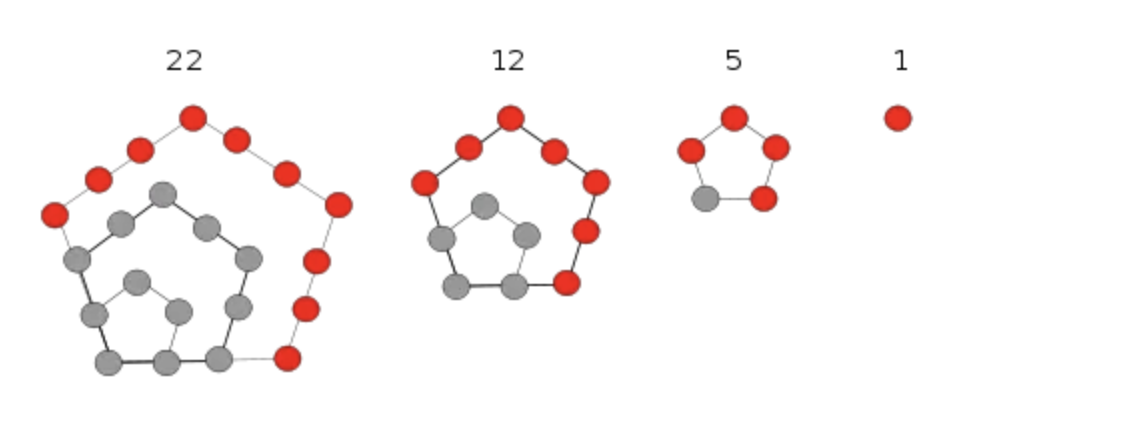
\includegraphics[scale=0.8]{五边形数1.png}

\begin{itemize}
    \item 
        五边形数
        \begin{quote}
            递推式: \(p_n = p_{n-1} + (3n - 2)\)。\\

            通项公式: \(p_n = \frac{3n^2 - n}{2}\)。\\

            简单来说, 大概就是一个边长为 \(n\) 的五边形, 里面套着一个边长为 \(n-1\) 的五边形, 以此类推。
            前面四项为: \(1,5,12,22\)。
        \end{quote}

    \item
        广义五边形数
        \begin{quote}
            如果把 \(n\) 的取值范围扩大到全体整数, 我们就能得到广义五边形数。
            我们按照 \(n = 0, 1, -1, 2, -2, \cdots \) 的顺序带入通项, 得到 \(0,1,2,5,7,12,15,22, \cdots\)。
        \end{quote}
    
    \item 
        五边形数定理
        \begin{quote}
            定义函数 \(\phi(x) = \prod_{k=1}^{inf} (1-x^k)\), 
            展开得到 \(\prod_{k=1}^{inf} (1-x^k) = \sum_{k=-inf}^{inf} (-1)^k x^{\frac{3k^2-k}{2}}\)
            注意 \(x\) 的次数, 这正是广义五边形数。\\

            将所得项按升幂排列, 得到 \(\phi(x) = 1 - x - x^2 + x^5 + x^7 - x^{12} - x^{15} + \cdots \)。
        \end{quote}   
        
    \item 
        整数拆分
        \begin{quote}
            求将正整数 \(n\) 拆分为若干个正整数的和 (允许同一个数使用多次, 即 1 + 2 和 2 + 1 等价) 的方案数。
            \\

            \begin{itemize}
                \item
                考虑两种 \( dp \), 可以根号分治, 时间复杂度是 \(O(n \sqrt{n})\)。

                \begin{quote}
                令 \( f_{i,j} \) 表示对于 \( i \) 拆分成若干个不大于 \( j \) 的数的方案数。则有转移:
                \(f_{i,j} = f_{i,j-1} + f_{i-j,j}\) 后面一项 \( f_{i-j,j} \) 可以看成一个背包一样,后面的状态对前面的状态有天然的累加效应,所以只需要考虑去掉一个 \( j \) 的情况;
                而前面一项则把我们转移从后一项的等于 \( j \) 升级成为不大于 \( j \)。
                \\
                
                令 \( g_{i,j} \) 表示对于 \( i \) 拆分成 \( j \) 个数的方案数。则有转移:
                \(g_{i,j} = g_{i-1,j-1} + g_{i-j,j}\)。
                \\
    
                前面一项表示新拆出一个 1 来,还是背包的那种"累加"思想,所以只需要考虑拆出一个 1 的情况;
                后面一项则表示不拆,而是把拆出的数全体都 \( +1 \),即本来的 \( 5 = 3 + 1 + 1 \) 转移到 \( 8 = 4 + 2 + 2 \)。
                \\
                
                注意此处不会存在"部分拆出来的数加了但是剩下的没加"或者"加的不一样",
                因为这两个状态都是可以归约到 \( i \) 较小的 \( g \) 上去所以不需要额外转移。
                \\
                \end{quote}

                \item 
                运用生成函数的解法。

                \begin{quote}
                    设 \(p(x)\) 为拆分 \(x\) 的方案数, 考虑 \(p(x)\) 的生成函数, 
                    \(\sum_{k=0}^{inf} p(k) x^k = \prod_{k=1}^{inf} \frac{1}{1 - x^k} = \frac{1}{\phi(x)}\)。
                    \\    

                    用五边形定理展开, 整理一下式子, 
                    \(\phi(x) \sum_{k=0}^{inf} p(k) x^k = (1 - x - x^2 + x^5 + x^7 - \cdots )(1 + p(1)x + p(2)x^2 + \cdots ) = 1\)。
                    。展开化简可以得到, \(p(k) - p(k-1) - p(k-2) + p(k-5) + p(k-7) - ... = 0\)。
                    \\
                    
                    根据这个式子我们就可以递归推算 \(p(x)\) 的值, 由于广义五边形数是 \(O(n^2)\) 级别,
                    因此递推式共有 \(O(\sqrt(n))\) 项, 综合时间复杂度就是 \(O(n \sqrt{n})\)。
                \end{quote}

            \end{itemize}
            
        \end{quote}
\end{itemize}

\subsection{错位排列}

\noindent 对应问题, $5$ 封不同的信, 编号 $1,2,3,4,5$, 现在要把这 $5$ 封信放在编号 $1,2,3,4,5$ 的信封中,
要求信封的编号与信的编号不一样。问有多少种不同的放置方式? \\

\noindent 假设考虑到第 \( n \) 个信封,初始时暂时把第 \( n \) 封信放在第 \( n \) 个信封中,然后考虑两种情况的递推:

\begin{itemize}
    \item 前面 \( n - 1 \) 个信封全部装错;
    \item 前面 \( n - 1 \) 个信封有一个没有装错其余全部装错。
\end{itemize} 


\noindent \textbf{前面 \( n - 1 \) 个信封全部装错}:
因为前面 \( n - 1 \) 个已经全部装错了,所以第 \( n \) 封只需要与前面任一个位置交换即可,总共有
\(
D_{n-1} \times (n - 1)
\)
种情况。\\

\noindent \textbf{前面 \( n - 1 \) 个信封有一个没有装错其余全部装错}:
考虑这种情况的目的在于,若 \( n - 1 \) 个信封中如果有一个没装错,那么把那个没装错的与 \( n \) 交换,即可得到一个全错位排列情况。\\


\noindent 其他情况,不可能通过一次操作来把它变成一个长度为 \( n \) 的错排。 \\

\noindent 于是可得,错位排列数满足递推关系:
\(
D_n = (n - 1)(D_{n-1} + D_{n-2})
\)。这里也给出另一个递推关系:
\(
D_n = nD_{n-1} + (-1)^n
\)。 \\

\noindent 错位排列对应数列的前几项为 $0,1,2,9,44,265$。 \\

\subsection{线性基}

\noindent 插入一个线性基是一个高斯消元的过程,插入一个数 x,从高位往下遍历,遍历到第 i 位的时候,如果 base[i] 已经存在一个向量了,
就把 x 替换为 \(x \oplus base[i]\),直到到达某位 base[i] 为空的时候插入进去,如果插入一个值 x 到线性基,从高处消元直到最后被消为 0,就认为线性基可以产出 0 值。\\

\noindent 线性基模板有两个标记,一个 zero 和一个 {is\_rebuild}。\\

\begin{itemize}
    \item zero 标记是判断一个 0 值是否可以由一个非空子集生成,它决定了能产生值的个数是 \(2^{cnt}\) 还是 \(2^{cnt} - 1\)。
    \item is\_rebuild 标记是在求解 k-th 问题的时候,需要重整线性基,抵消低位的共享,保持高位的独立,方便使用二进制枚举确定 k-th 的值。
\end{itemize}

\noindent 对于其他的问题,比如最值问题,就不需要 rebuild,求解最值的过程是一个贪心的过程。\\

\begin{lstlisting}
// created on 24-8-23

const int MAXN=64;
struct Linear_Basis {
    ll cnt=0;
    ll d[MAXN];
    ll base[MAXN]={0};
    bool zero=false, is_rebuild=false;
    void init() {
        zero = false;
        is_rebuild = false;
        for (int i = 0; i <= MAXN; i++) base[i] = 0;
    }
    void rebuild() { 
        // 重构线性基方便查找 kth 值
        for (int i = 0; i <= 62; i++) {
            for (int j = i - 1; j >= 0; j--) {
                if (base[i] & (1ll << j)) {
                    base[i] ^= base[j];
                }
            }
        }
        for (int i = 0; i <= 62; i++) if (base[i]) {
            d[cnt ++] = base[i];
        }
    }
    bool insert(ll x) { 
        // 插入线性基
        for (int i = MAXN - 1; ~i; i--) {
            if (x & (1LL << i)) {
                if(!base[i]) {
                    base[i] = x;
                    return true;
                }
                else x ^= base[i];
            }
        }
        zero = true;
        is_rebuild = false;
        return false;
    }
    bool check(ll x) { 
        // 查找某个值能否在线性基里面产生
        if (!x) return zero;
        for (int i = MAXN - 1; i >= 0; i--) if (x & (1LL << i)) {
            if (!base[i]) return false;
            x ^= base[i];
        }
        return true;
    }
    ll qmax(ll s) { 
        // 与 s 异或能在线性基里面产生的最大值
        for(int i = MAXN - 1; i >= 0; i--) {
            s = max(s, s^base[i]);
        }
        return s;
    }
    ll qmin() { // 线性基产生的最小值
        if (zero) return 0;
        for (int i = 0; i <= 63; i++) if (base[i]) {
            return base[i];
        }
    }
    ll qkth(ll x) { 
        // 查找第 k 小值 0....1ll<<cnt
        if (!is_rebuild) {
            rebuild();
            is_rebuild = true;
        }
        if (x >= (1ll << cnt)) return -1;
        ll res = 0;
        for (int i = 0; i <= 62; i++)
        if (x & (1ll << i)) res ^= d[i];
        return res;
    }
    friend Linear_Basis operator + (const Linear_Basis &u,const Linear_Basis &v) { 
        // merge
        Linear_Basis ret;
        for(int i = 63; i >= 0; i--){
            if (u.base[i]) ret.insert(u.base[i]);
            if (v.base[i]) ret.insert(v.base[i]);
        }
        ret.zero = u.zero | v.zero;
        ret.is_rebuild = false;
        return ret;
    }
}l1;
\end{lstlisting}

\subsection{高斯消元}

\subsubsection{解一般方程组}

\noindent 解方程的三种结果:

\begin{itemize}
    \item 唯一解:全部主元行对应变量。
    \item 无限解:存在自由变量行 0 = 0。
    \item 无解:出现方程矛盾,1 = 0。
\end{itemize}

\begin{lstlisting}
// created on 25-4-30

// 取模高斯消元 O(N^2)
ll ksm(ll a, ll b) {
    ll ans = 1;
    a %= mod;
    while(b) {
        if(b & 1) ans = ans * a % mod;
        a = a * a % mod;
        b >>= 1;
    }
    return ans;
}

// guass(a,n,n);

ll guass(ll a[][N], ll n, ll m) { 
    ll cnt = 0, ans = 1;
    for(int c = 0;c < min(n, m);c ++) {
        int r = c;
        for(int i = r + 1;i < n;i ++) {
            if(a[i][c] > a[r][c]) {
                r = i;
            }
        }
        cnt += r != c;
        swap(a[c], a[r]);
        if(a[r][c] == 0) {
            return 0;
        }
        ans = ans * a[c][c] % mod;
        for(int i = 0;i < n;i ++) if(i != c) {
            ll t = a[i][c] * ksm(a[c][c], mod - 2);
            t %= mod;
            for(int j = c;j < m;j ++) {
                a[i][j] -= t * a[c][j] % mod;
                a[i][j] = (a[i][j] % mod + mod);
                a[i][j] %= mod;
            }
        }
    }
    if(cnt & 1) ans = mod - ans;
    return ans;
}
\end{lstlisting}

\noindent 输出一个包含 $N$ 个方程 $N$ 个未知数的线性方程, 系数与常数均为实数 (两位小数)。
求解这个方程组, 如果存在唯一解, 则输出所有 $N$ 个未知数的解, 
结果保留两位小数, 如果无数解输出 inf, 如果无解, 输出 No。\\

\begin{lstlisting}
// created on 24-8-23

const int N = 110;
const double eps = 1e-8;
LL n;
double a[N][N];
LL gauss(){
    LL c, r;
    for (c = 0, r = 0; c < n; c ++ ){
        LL t = r;
        //找到绝对值最大的行
        for (int i = r; i < n; i ++ ) {
            if (fabs(a[i][c]) > fabs(a[t][c])) {
                t = i;
            }
            if (fabs(a[t][c]) < eps) continue;
        }
        //将绝对值最大的一行换到最顶端
        for (int j = c; j < n + 1; j ++ ) {
            swap(a[t][j], a[r][j]);
        }
        //将当前行首位变成 1
        for (int j = n; j >= c; j -- ) {
            a[r][j] /= a[r][c]; 
        }
        //将下面列消成 0
        for (int i = r + 1; i < n; i ++ ) {
            if (fabs(a[i][c]) > eps) {
                for (int j = n; j >= c; j -- ) {
                    a[i][j] -= a[r][j] * a[i][c];
                }
            }
        }
        r ++;
    }
    if (r < n){
        for (int i = r; i < n; i ++ ) {
            if (fabs(a[i][n]) > eps) {
                return 2;
            }
        }
        return 1;
    }
    for (int i = n - 1; i >= 0; i -- ) {
        for (int j = i + 1; j < n; j ++ ) {
            a[i][n] -= a[i][j] * a[j][n];
        }
    }
    return 0;
}
int main(){
    cin >> n;
    for (int i = 0; i < n; i ++ )
        for (int j = 0; j < n + 1; j ++ )
                cin >> a[i][j];
    LL t = gauss();
    if (t == 0){
        for (int i = 0; i < n; i ++ ){
            if (fabs(a[i][n]) < eps) {
                a[i][n] = abs(a[i][n]);
            }
            printf("%.2lf\n", a[i][n]);
        }
    }
    else if (t == 1) cout << "Infinite_group_solutions\n";
    else cout << "No_solution\n";
    return 0;
}
\end{lstlisting}

\subsubsection{解异或方程组}

\noindent 异或方程组一部分情况是求解自由变量的个数。
求解自由变量的个数与等式右边的情况无关,主要是跟矩阵的秩相关。\\

\begin{lstlisting}
// created on 25-9-23

const int N = 210;
int n;
bitset<N> a[N];

int gauss() {
	int r, c;
	for (r = 1, c = 1; c <= n; c ++ ) {
		int t = r;
		for (int i = r + 1; i <= n; i ++ ) {
			if (a[i][c]) {
				t = i;
			}			
		}
		if (!a[t][c]) {
			continue;
		}
		swap(a[t], a[r]);

		for (int i = r + 1; i <= n; i ++ ) {
			for (int j = n + 1; j >= c; j -- ) {
				if (a[i][c]) {
					a[i] ^= a[r];
				}
			} 
		}
		r ++;
	}

	// 返回的是自由变量的数量
	int res = 0;
	if (r < n + 1) {
		for (int i = r; i <= n; i ++ ) {
			if (a[i][n + 1]) {
				return -1;
			}
			res ++;
		}
	}

	return res;
}
\end{lstlisting}

\subsection{矩阵四则运算}

\begin{lstlisting}
// created on 24-8-23

const int SIZE = 2;
struct Matrix {
    ll M[SIZE + 2][SIZE + 2];
    void clear() { 
        memset(M, 0, sizeof(M)); 
    }
    void reset() { //初始化
        clear();
        for (int i = 1; i <= SIZE; ++i) M[i][i] = 1;
    }
    Matrix friend operator*(const Matrix &A, const Matrix &B) {
        Matrix Ans;
        Ans.clear();
        for (int i = 1; i <= SIZE; ++i) {
            for (int j = 1; j <= SIZE; ++j) {
                for (int k = 1; k <= SIZE; ++k) {
                    Ans.M[i][j] = (Ans.M[i][j] + A.M[i][k] * B.M[k][j]) % mod;
                }
            }
        }
        return Ans;
    }
    Matrix friend operator+(const Matrix &A, const Matrix &B) {
        Matrix Ans;
        Ans.clear();
        for (int i = 1; i <= SIZE; ++i) {
            for (int j = 1; j <= SIZE; ++j) {
                Ans.M[i][j] = (A.M[i][j] + B.M[i][j]) % mod;
            }
        }
        return Ans;
    }
};
inline int mypow(LL n, LL k, int p = MOD) {
    LL r = 1;
    for (; k; k >>= 1, n = n * n % p) {
        if (k & 1) r = r * n % p;
    }
    return r;
}
bool ok = 1;
Matrix getinv(Matrix a) { //矩阵求逆
    int n = SIZE, m = SIZE * 2;
    for (int i = 1; i <= n; i++) a.M[i][i + n] = 1;
    for (int i = 1; i <= n; i++) {
        int pos = i;
        for (int j = i + 1; j <= n; j++) {
            if (abs(a.M[j][i]) > abs(a.M[pos][i])) pos = j;
        }
        if (i != pos) swap(a.M[i], a.M[pos]);
        if (!a.M[i][i]) {
            puts("No_Solution");
            ok = 0;
        }
        ll inv = q_pow(a.M[i][i], mod - 2);
        for (int j = 1; j <= n; j++) {
            if (j != i) {
                ll mul = a.M[j][i] * inv % mod;
                for (int k = i; k <= m; k++)
                a.M[j][k] = ((a.M[j][k] - a.M[i][k] * mul) % mod + mod) % mod;
            }
        }
        for (int j = 1; j <= m; j++) a.M[i][j] = a.M[i][j] * inv % mod;
    }
    Matrix res;
    res.clear();
    for (int i = 1; i <= n; i++) {
        for (int j = 1; j <= m; j++) {
            res.M[i][j] = a.M[i][n + j];    
        }
    }
    return res;
}
\end{lstlisting}

\subsection{矩阵快速幂}

\begin{lstlisting}
    // created on 24-8-23
    const int N = 110, mod = 1e9 + 7;
    LL n, k, a[N][N], b[N][N], t[N][N];
    void matrixQp(LL y){
        while (y){
            if (y & 1){
                memset(t, 0, sizeof t);
                for (int i = 1; i <= n; i ++ ) {
                    for (int j = 1; j <= n; j ++ ) {
                        for (int k = 1; k <= n; k ++ ) {
                            t[i][j] = (t[i][j] + (a[i][k] * b[k][j]) % mod) % mod;
                        }
                    }
                }
                memcpy(b, t, sizeof t);
            }
            y >>= 1;
            memset(t, 0, sizeof t);
            for (int i = 1; i <= n; i ++ )
            for (int j = 1; j <= n; j ++ )	
            for (int k = 1; k <= n; k ++ )
            t[i][j] = ( t[i][j] + (a[i][k] * a[k][j]) % mod ) % mod;
            memcpy(a, t, sizeof t);
        }
    }
    int main(){
        cin >> n >> k;
        for (int i = 1; i <= n; i ++ )
        for (int j = 1; j <= n; j ++ ){
            cin >> b[i][j];
            a[i][j] = b[i][j];
        }
        matrixQp(k - 1);
        for (int i = 1; i <= n; i ++ )
        for (int j = 1; j <= n; j ++ )
        cout << b[i][j] << " \n"[j == n];
        return 0;
    }
    
\end{lstlisting}

\subsection{生成函数}

\subsubsection{普通生成函数}

\begin{itemize}
\item
    定义:\(F(x) = \sum_{n\geq0} a_n x^n\)。
\item
    问题1:有 \(n\) 种物品,每种物品有 \(a_i\) 个,问取 \(m\)
    个物品的组合数。(多重集组合数)
\end{itemize}

\begin{quote}
假设第 \(i\) 种物品的数量有 \(a_i\)
个,我们可以这样构造这个物品的多项式:\((1+x^1+x^2+...+x^{a_i})\)。一共有
\(n\) 个这样的多项式,我们把它们乘起来,\(x^m\) 的系数即为答案。
\end{quote}

\begin{itemize}
\item
    问题2:有面值为 \(1,2,5\) 的硬币分别有 \(a_1,a_2,a_3\)
    枚,问这些面值的硬币不能组成的最小面值是多少。
\end{itemize}

\begin{quote}
这种情况下构造取到的价值的生成函数为:
\((1+x^1+x^2+...+x^{a_1})*(1+x^2+...+x^{2a_2})*(1+x^5+...+x^{5a_3})\),与前面不同,这种问题的实质是考虑物品的权重,上面物品的权重为
1,而这里对于价值来说,明显 1,2,5 块钱的权重不同。
\end{quote}

\subsubsection{指数生成函数}

\begin{itemize}
\item
    定义:\(F(x)=\sum_{n\geq0} a_n \frac{x^n}{n!}\)。
\item
    卷积:\textless{}\(a_i\)\textgreater{} 的指数生成函数 与
    \textless{}\(b_i\)\textgreater{} 的指数生成函数 卷积得到
    \(<\sum_{i=0}^n C_n^i a_i b_{n-i}>\) 的指数生成函数。
\item
    问题 1: 有 \(n\) 种物品,每种物品有 \(a_i\) 个,问取 \(m\)
    个物品的排列数。(多重集排列数)
\end{itemize}

\begin{quote}
比如说有物品 A 和 物品 B,假设取了 3 个 A 和 1 个 B 的排列数为
\(\frac{m!}{3! \ 1!}=4\),即 \{AAAB,AABA,ABAA,BAAA\}。

同普通生成函数,构造的指数生成函数为
\((1 + \frac{x^1}{1!} + \frac{x^2}{2!} + ... + \frac{x^{a_1}}{a_1!}) * ... * (1 + \frac{x^1}{1!} + \frac{x^2}{2!} + .. . + \frac{x^{a_n}}{a_n!})\),求
\(\frac{x^m}{m!}\) 的系数即可。

计算的时候
\(\frac{x^{b_1}}{b_1!}*\frac{x^{b_2}}{b_2!}*...*\frac{x^{b_n}}{b_n!}=\frac{1}{b_1*b_2*...*b_n}*x^m\),其中所有满足
\(b_1+b_2+...+b_n=m\) 的项数之和为
\(\frac{k}{b_1*b_2*...*b_n}*x^m\),然后给系数乘一个 \(m!\)
即可得到答案。
\end{quote}

\subsubsection{生成函数的应用}

\begin{itemize}
\item
泰勒展开式

\begin{quote}
\begin{enumerate}
\def\labelenumi{\arabic{enumi}.}
\item
\(\frac{1}{1-x}=1+x+x^2+...\)
\item
\(\frac{1}{1-x^2}=1+x^2+x^4+...\)
\item
\(\frac{1}{(1-x)^2} = 1 + 2x + 3x^2 + ...  \)(1)等式两边求导数
\item
\(e^x = 1 + \frac{x^1}{1!} + \frac{x^2}{2!} + ... \)
\item
\(e^{-x} = 1 - \frac{x^1}{1!} + \frac{x^2}{2!} - ... \)(4) 等式换元
\end{enumerate}

根据 4,5 可以分离出奇偶项。
\end{quote}
\item
有穷序列的生成函数
\begin{quote}
\begin{enumerate}
\def\labelenumi{\arabic{enumi}.}
\item
\(1 + x + x^2 = \frac{1-x^3}{1-x}\)
\item
\(1 + x + x^2 + x^3 = \frac{1-x^4}{1-x}\)
\end{enumerate}
\end{quote}

\item
广义二项式定理
\begin{quote}
\(\frac{1}{(1-x)^n} = \sum_{i=n}^{inf} C_{n+i-1}^i x^i\)
\end{quote}
\end{itemize}

\subsubsection{补充证明}

\begin{quote}
\begin{enumerate}
\def\labelenumi{\arabic{enumi}.}
\item
    \(F(x) = \frac{1}{1-x} = 1 + x + x^2 + ...\) 是怎么来的。

    不太严谨的证明:这是一个等比数列,而等比数列的求和公式为
    \(\frac{a_0}{1-q}(1-q^n)\),当 \(q<1,n\)-\textgreater{}\(inf\)
    时,这个等比数列的值为 \(\frac{1}{1-q}\)。但是 \(q>1\)
    的情况是发散的。\\
\item
    \(F(x) = a_0 + a_1 * x + a_2 * x^2 + ... \) 与
    \(G(x) = 1 + x + x^2 + ...\) 作卷积得到的是
    \textless{}\(\sum_{i=1}^n  a_i\)\textgreater{} 的生成函数,说人话就是做了一个前缀和。

    利用这个可以推导很多东西,比如:

    \(W(x) = \frac{1+x}{(1-x)^3} = 1 + 4 x + 9 x^2 + 16 x^3 + ...\)\ \\
\item
    用函数 (多项式代数) 表示各种数列:

    \begin{itemize}
    \item
    \(c * F(x)\) -\textgreater{} 数列倍增。
    \item
    \(x * F(x)\) -\textgreater{} 数列右移。
    \item
    \([F(x) - f(0)] / x\) -\textgreater{} 数列左移。
    \item
    \(F_1(x) + F_2(x)\) -\textgreater{} 数列求和。
    \item
    \(F'(x)\) -\textgreater{} 数列乘幂次 + 数列左移。
    \item
    \(F_1(x) * F_2(x)\) -\textgreater{} 数列卷积。
    \\
    \end{itemize}

\item
    Fibonacci 的生成函数为:\(F(x) = \frac{x}{1-x-x^2}\)。

    假设 Fibonacci 的生成函数为:

    \(F(x) = f(0) + f(1)*x + f(2)*x^2 + ...\) (1)\\

    那么也有:

    \(x * F(x) = f(0) * x + f(1) * x^2 + f(2) * x^3 + ...\) (2)

    \(x^2 * F(x) = f(0) * x^2 + f(1) * x^3 + f(2) * x^4 + ...\) (3)\\

    然后 (1) - (2) - (3):

    \(F(x) * (1 - x - x^2) = f(0) + (f(1) - f(0)) * x + (f(2) - f(1) - f(0)) * x^2 + (f(3) - f(2) - f(1)) * x^3 + ...\) \\

    其中 \(f(0) = 0, f(1) = 1, f(2) = 1\) 带入后得到:

    \(F(x)*(1-x-x^2) = x\)。\\
\item
    \(x * F(x) = \frac{x}{1-x} = x + x^2 + x^3 + ...\)。

    那么也有于 \(\frac{x^2}{1-x} = x^2 + x^3 + x^4 + ...\),从而
    \(\frac{1-x^2}{1-x} = 1 + x\)。看上去有点蠢。
\end{enumerate}

\end{quote}
    

\subsection{阶数}

\begin{itemize}
\item
    阶数
    \begin{quote}
    满足 \(a^n \equiv 1\ (mod \ m)\) 的最小正整数 \(n\),称为 \(a\) 的模
    \(m\) 的阶,记为 \(\delta_m(a)\)。
    
    例如:\(2^3 \equiv 1\ (mod\ 7)\),当
    \(a = 2, m = 7\),\(\delta_m(a) = 3\)。
    \end{quote}
\item 
    性质
    \begin{quote}
    \begin{enumerate}
        \def\labelenumi{\arabic{enumi}.}
        \item 
            \(a, a^2, a^3, \cdots a^{\delta_m(a)}\) 模 \(m\) 两两不同余。
        \item 
            若 \(a^n \equiv 1 \ (mod \ m)\), 则 \(\delta_m(a) \ | \ n\)。
        \item 
            若 \(a^r \equiv a^t \ (mod \ m)\), 则 \(r \equiv t \ (mod \ \delta_m(a))\)。
        \item 
            若 \(gcd(a,m)=1\), 则 \(\delta_m(a^k) = \frac{\delta_m(a^k)}{gcd(\delta_m(a),k)}\)。
    \end{enumerate}        
    \end{quote}
\end{itemize}

\subsection{原根}

\begin{itemize}
\item
    欧拉定理

    \begin{quote}
    对于任意
    \(a \in Z, m \in N^*, gcd(a,m)=1, a^{\varphi(m)} \equiv 1\ (mod\ m)\)。
    \end{quote}
    
\item
    定义

    \begin{quote}
    对于模数 \(m\) 来说,原根 \(a\) 满足 \(\delta_m(a) = \varphi(m)\)。
    通俗点说 \(a^1, a^2, \cdots a^{\varphi(m)}\) 在模 \(m\) 意义下各不相同。
    
    例如:
    
    \begin{enumerate}
    \def\labelenumi{\arabic{enumi}.}
    \item
        \(a=2,m=7,\delta_m(a) = 3\),而 \(\varphi(7)=6\)。故 \(a=2\) 不为
        \(m=7\) 的原根。
    \item
        \(a=3,m=7,\delta_m(a)=6\),而 \(\varphi(7)=6\)。故 \(a=3\) 为 \(m=7\)
        的原根。
    \end{enumerate}
    \end{quote}
\item 
    性质
    \begin{quote}
    \begin{enumerate}
    \def\labelenumi{\arabic{enumi}.}
    \item 
        若 \(m>1,gcd(a,m)=1\), 正整数 \(d\) 满足 \(a^d \equiv 1 \ (mod \ m)\), 
        则 \(\delta_d\) 整除 \(d \)。
    \item
        模 \(m\) 有原根的充要条件是 \(m=2,4,p^n,2p^n\), 其中 \(p\) 是奇质数, \(n\) 是任意正整数。
    \item
        如果模 \(m\) 存在原根, 那么它一定拥有 \(\varphi(\varphi(m))\) 个原根。
    \end{enumerate}
    \end{quote}
\item 
    原根数量
    \begin{quote}
        设 \( a \) 是模 \( m \) 的一个原根,则其幂序列 \( a^1, a^2, \ldots, a^{\varphi(m)} \) 在模 \( m \) 下两两不同(否则与 \( \delta_m(a) \) 的最小循环节定义矛盾)。

        \begin{enumerate}
            \item 
            取任意正整数 \( t \) 满足 \( \gcd(t, \varphi(m)) = 1 \)。
        
            \item 
            考虑反证法:假设存在 \( 1 \leq i < j \leq \varphi(m) \),使得
            \(
            i \cdot t \equiv j \cdot t \pmod{\varphi(m)}.
            \)
            则可得:
            \(
            (j - i)t \equiv 0 \pmod{\varphi(m)}.
            \)
            由于 \( t \) 与 \(\varphi(m)\) 互质,必有:
            \(
            \varphi(m) \mid (j - i).
            \)
            但 \( 1 \leq j - i < \varphi(m) \),矛盾。因此,\( \{ t, 2t, \ldots, \varphi(m)t \} \) 在模 \(\varphi(m)\) 下两两不同。
        
            \item 
            由上述结论,序列 \( a^{t}, a^{2t}, \ldots, a^{\varphi(m)t} \) 在模 \( m \) 下亦两两不同,故 \( a^t \) 是模 \( m \) 的原根。
        
            \item 
            满足 \( \gcd(t, \varphi(m)) = 1 \) 的 \( t \) 共有 \(\varphi(\varphi(m))\) 个,因此模 \( m \) 的原根数量为:
            \(
            \varphi(\varphi(m)).
            \)
        
            \item 
            若存在其他原根 \( b \),则必存在 \( k \) 使得 \( b \equiv a^k \pmod{m} \),且 \( \gcd(k, \varphi(m)) = 1 \)。由鸽巢原理,所有原根均属于此形式。
        \end{enumerate}
    \end{quote}
\item 
    应用: 乘法转化为加法
    \begin{quote}
        若 \(p\) 有原根, 根据阶的性质 1 和原根的定义, 若 \(g\) 是 \(p\) 的原根, \(1 \leq k \leq \varphi(p)\),
        \(g^k \ (mod \ p)\) 能生成 [1, p - 1] 中 \(\varphi(p)\) 个数。
        换句话说就是 \(g^1, g^2, \cdots, g^{\varphi(p)} \ (mod \ p)\) 与 [1, p - 1] 中的数形成了单射。
        当 \(p\) 是质数时, 就形成了双射, 一一对应。 \\

        若 \(p\) 是质数, \(1 \leq a,b\), 则 \(a * b = g^{Ind_{g_a}+Ind_{g_b}} \ (mod \ p)\)。
        因此求出 \(p\) 的原根 \(g\), 然后我们就可以把原序列 \(a[i]\) 变成 \(g^{b[i]}\), 从而实现把乘法变为加法。
        即 \(a[i]*a[j]=a[k] \ (mod \ p)\) 变为 \(b[i] + b[j] = b[k] \ (mod \ p-1)\), 注意特判 0。\\

        PS: \(Ind\) 为离散对数。
    \end{quote}
\end{itemize}


\subsection{FFT}

\noindent 注意 Comp 类是一个 Double,输出 $\lfloor x + 0.5 \rfloor$。

\begin{lstlisting}
// created on 25-4-30

using Comp = std::complex<double>;  // STL complex

constexpr Comp I(0, 1);  // i
constexpr int MAX_N = 1 << 20;

Comp tmp[MAX_N];

// rev=1,DFT; rev=-1,IDFT
void DFT(Comp* f, int n, int rev) {
    if (n == 1) return;
    for (int i = 0; i < n; ++i) tmp[i] = f[i];
    // 偶数放左边,奇数放右边
    for (int i = 0; i < n; ++i) {
        if (i & 1) {
            f[n / 2 + i / 2] = tmp[i];
        } else {
            f[i / 2] = tmp[i];
        }
    }
    Comp *g = f, *h = f + n / 2;
    // 递归 DFT
    DFT(g, n / 2, rev), DFT(h, n / 2, rev);
    // cur 是当前单位复根,对于 k = 0 而言,它对应的单位复根 w^0_n = 1。
    // step 是两个单位复根的差,即满足 w^k_n = step*w^{k-1}*n,
    // 定义等价于 exp(I*(2*M_PI/n*rev))
    Comp cur(1, 0), step(cos(2 * M_PI / n), sin(2 * M_PI * rev / n));
    for (int k = 0; k < n / 2; ++k) {  
        // F(w^k_n) = G(w^k*{n/2}) + w^k*n * H(w^k_{n/2})
        tmp[k] = g[k] + cur * h[k];
        // F(w^{k+n/2}*n) = G(w^k*{n/2}) - w^k_n * H(w^k_{n/2})
        tmp[k + n / 2] = g[k] - cur * h[k];
        cur *= step;
    }
    for (int i = 0; i < n; ++i) f[i] = tmp[i];
}
\end{lstlisting}

\subsection{NTT}

\noindent 原根代替复数根: \\

\begin{quote}
    在加减乘除的运算中,我们拥有使用模数等效小数的方法。
    这里我们使用原根代替复数根,可以证明在适合模数下是等效的。

    \(g_n^k = (G^{\frac{p-1}{n}})\ (mod \ p)\)。例如:\(p = 17, G = 3, n = 8,g_8^k = (3^{\frac{17-1}{8}})^k \% 17\)。
    其中这里的 \(p\) 是模数,\(G\) 为模数的原根,\(n\) 为分成 \(n\) 等分。

    注意一点,由于 \(\frac{p-1}{n}\) 不能下取整,\(p\) 尽量选择
    \(p_0 \times 2^k + 1\) 这种类型的质数。
\end{quote}
    
\begin{lstlisting}
constexpr int P = 998244353;

int power(int a, int b) {
    int res = 1;
    for (; b; b /= 2, a = 1LL * a * a % P) {
        if (b % 2) {
            res = 1LL * res * a % P;
        }
    }
    return res;
}

vector<int> rev, roots {0, 1};

void dft(vector<int> &a) {
    int n = a.size();
    if (int(rev.size()) != n) {
        int k = __builtin_ctz(n) - 1;
        rev.resize(n);
        for (int i = 0; i < n; i++) {
            rev[i] = rev[i >> 1] >> 1 | (i & 1) << k;
        }
    }
    for (int i = 0; i < n; i++) {
        if (rev[i] < i) {
            swap(a[i], a[rev[i]]);
        }
    }
    if (roots.size() < n) {
        int k = __builtin_ctz(roots.size());
        roots.resize(n);
        while ((1 << k) < n) {
            int e = power(31, 1 << (__builtin_ctz(P - 1) - k - 1));
            for (int i = 1 << (k - 1); i < (1 << k); i++) {
                roots[2 * i] = roots[i];
                roots[2 * i + 1] = 1LL * roots[i] * e % P;
            }
            k++;
        }
    }

    for (int k = 1; k < n; k *= 2) {
        for (int i = 0; i < n; i += 2 * k) {
            for (int j = 0; j < k; j++) {
                int u = a[i + j];
                int v = 1LL * a[i + j + k] * roots[k + j] % P;
                a[i + j] = (u + v) % P;
                a[i + j + k] = (u - v) % P;
            }
        }
    }
}

void idft(vector<int> &a) {
    int n = a.size();
    reverse(a.begin() + 1, a.end());
    dft(a);
    int inv = (1 - P) / n;
    for (int i = 0; i < n; i++) {
        a[i] = 1LL * a[i] * inv % P;
    }
}

vector<int> mul(vector<int> a, vector<int> b) {
    int n = 1, tot = a.size() + b.size() - 1;
    while (n < tot) {
        n *= 2;
    }
    if (tot < 128) {
        vector<int> c(a.size() + b.size() - 1);
        for (int i = 0; i < a.size(); i++) {
            for (int j = 0; j < b.size(); j++) {
                c[i + j] = (c[i + j] + 1LL * a[i] * b[j]) % P;
            }
        }
        return c;
    }
    a.resize(n);
    b.resize(n);
    dft(a);
    dft(b);
    for (int i = 0; i < n; i++) {
        a[i] = 1LL * a[i] * b[i] % P;
    }
    idft(a);
    a.resize(tot);
    return a;
}
\end{lstlisting}

\newpage

\fancyhead[L]{计算几何}
\section{计算几何}

\subsection{结论}

\begin{itemize}
\item 边心距是指正多边形的外接圆圆心到正多边形某一边的距离,边长为 \( s \) 的正 \( n \) 角形的边心距公式为 \( a = \frac{t}{2 \cdot \tan \frac{\pi}{n}} \),外接圆半径为 \( R \) 的正 \( n \) 角形的边心距公式为 \( a = R \cdot \cos \frac{\pi}{n} \);

\item 三角形外接圆半径为 \( \frac{a}{2 \sin A} = \frac{abc}{4S} \),其中 \( S \) 为三角形面积,内切圆半径为 \( \frac{2S}{a+b+c} \);

\item 由小正三角形拼成的大正三角形,耗费的小三角形数量即为构成一条边的小三角形数量的平方。

\item 正 \( n \) 边形圆心角为 \( \frac{360^\circ}{n} \),圆周角为 \( \frac{180^\circ}{n} \)。定义正 \( n \) 边形上的三个顶点 \( A, B \) 和 \( C \)(可以不相邻),使得 \( \angle ABC = \theta \),当 \( n \leq 360 \) 时,\( \theta \) 可以取 \( 1^\circ \) 到 \( 179^\circ \) 间的任何一个整数。

\item 某一点 \( B \) 到直线 \( AC \) 的距离公式为 \( \frac{|B^A \times BC|}{|AC|} \),等价于 \( \frac{|aX + bY + c|}{\sqrt{a^2 + b^2}} \)。

\item \( \tan(y / x) \) 函数仅用于计算第一、四象限的值,而 \( \tan(2y, x) \) 则允许计算所有四个象限的正反切,在使用这个函数时,需要尽量保证 \( x \) 和 \( y \) 的类型为整数组,如果使用浮点数,实测会慢十倍。

\item 在平面上有奇数个点 \( A_0, A_1, \ldots, A_n \) 以及一个点 \( X_0 \),构造 \( X_1 \) 使得 \( X_0, X_1 \) 关于 \( A_0 \) 对称。构造 \( X_2 \) 使得 \( X_1, X_2 \) 关于 \( A_1 \) 对称。……构造 \( X_j \) 使得 \( X_{j-1}, X_j \) 关于 \( A_{j-1} \) mod \( n \) 对称。那么周期为 \( 2n \),即 \( A_0 \) 与 \( A_{2n} \) 共点。\( A_1 \) 与 \( A_{2n+1} \) 共点 \text{See}。

\item 已知 \( A(x_A, y_A) \) 和 \( X(x_x, y_x) \) 两点及这两点的坐标,构造 \( Y \) 使得 \( X, Y \) 关于 \( A \) 对称,那么 \( Y \) 的坐标为 \( (2 \cdot x_A - x_x, 2 \cdot y_A - y_x) \)。

\item 海伦公式:已知三角形三边长 \(a, b, c\), 定义 \(p = \frac{a+b+c}{2}\), 则 \(S_\triangle = \sqrt{p(p-a)(p-b)(p-c)}\)
。在使用时需要注意越界问题,本质是铅锤定理,一般多使用叉乘计算三角形面积而不使用该公式。

\item 棱台体积: \(V = \frac{1}{3}(S_1 + S_2 + \sqrt{S_1 S_2}) \cdot h\), 其中 \(S_1, S_2\) 为上下底面积。
\item 正棱台侧面积: \(\frac{1}{2}(C_1 + C_2) \cdot L\), 其中 \(C_1, C_2\) 为上下底周长,\(L\) 为斜高(上下底对应的平行边的距离)。
\item 球面积: \(4\pi r^2\)。
\item 球体积: \(\frac{4}{3}\pi r^3 \)。
\item 正三角形面积: \(\frac{\sqrt{3}a^2}{4}\)。
\item 正四面体面积: \(\frac{\sqrt{2}a^3}{12}\)。
\item 设扇形对应的圆心角弧度为: \(\theta\), 则面积为 \(S = \frac{\theta}{2} \cdot R^2\)。
\item 欧拉公式: \(V - E + F - C + 1\), 点 - 边 + 面(二维: 区域) = 连通块数列 + 1。
\begin{quote}
    在二维的情况下,一个圆上四个点被认为是在同一个连通块上;
    如果一个圆与其他的圆相离没有形成交点,就算一个点自环。    
\end{quote}
\item 皮克定理: 绘制在方格上的多边形面积公式可以表示为 \(S = n + \frac{s}{2} - 1\), 
其中 \(n\) 表示多边形内部的点数, \(s\) 表示多边形边界上的点数。一条线段上的点数为 \(gcd(|x_1 - x_2|, |y_1 - y_2|) + 1\)。
\begin{lstlisting}
// created on 24-8-23
int onPolygonGrid(vector<Point<int>> p) { // 多边形上
    int n = p.size(), ans = 0;
    for (int i = 0; i < n; i++) {
        auto a = p[i], b = p[(i + 1) % n];
        ans += gcd(abs(a.x - b.x), abs(a.y - b.y));
    }
    return ans;
}
int inPolygonGrid(vector<Point<int>> p) { // 多边形内
    int n = p.size(), ans = 0;
    for (int i = 0; i < n; i++) {
        auto a = p[i], b = p[(i + 1) % n], c = p[(i + 2) % n];
        ans += b.y * (a.x - c.x);
    }
    ans = abs(ans);
    return (ans - onPolygonGrid(p)) / 2 + 1;
} 
\end{lstlisting}
\end{itemize}

\subsection{模版细节}

\noindent 使用的 dls 的计算几何的模版, 有一些实现细节和使用细节:

\begin{enumerate}
    \item 精度误差相关:
    \begin{quote}
        如果点的范围是 \( w \),那么范围误差应该是 \( 1e-2w \)。

        没有特别标注的函数精度误差为 \( db \)。

        \( db = 1e-15, \quad ld = 1e-18. \)\\
    \end{quote}
    \item 输入输出细节:
    \begin{quote}
    \begin{enumerate}
        \item 没有 spj 的话输出要加上一个 \texttt{eps},以防出现 \texttt{-0.0000}。
    
        \item 圆相切弧度,\( t > tr + eps \) 表示左弧度大于右弧度且不包含相切的情况。
        
        \item \texttt{printf} 好像不太能输出 \texttt{long double},只能强制转换成 \texttt{double} 再输出。
        
        \item 有时候精度要求不大的时候开 \texttt{long double} 可能会出点事。\\
    \end{enumerate}
    \end{quote}
    \item 点积叉积相关:
    \begin{quote}
        点积运算:
        \[ \text{dot}(a, b) = a \cdot b \]
        \[ \text{dot} > 0: \theta < \frac{\pi}{2} \]
        \[ \text{dot} = 0: \theta = \frac{\pi}{2} \]
        \[ \text{dot} < 0: \theta > \frac{\pi}{2} \]
        
        叉积运算:
        \[ \text{det}(a, b) = a \times b \]
        \[ \text{det} > 0: b \text{ 在 } a \text{ 逆时针方向} \]
        \[ \text{det} = 0: \text{共线} \]
        \[ \text{det} < 0: b \text{ 在 } a \text{ 顺时针方向} \]
        
        叉积几何意义:
        \[ \text{cross}(p_1, p_2, p_3) = |(p_2 - p_1) \times (p_3 - p_1)| \]      
    \end{quote}
    \begin{quote}
        角度正负相关:      
    \begin{itemize}
        \item \( \text{cross}(p_1, p_2, p_3) > 0 \) 的情况:逆时针方向。
        \[
        \begin{array}{c}
        p_3 \\
        p_1 \quad p_2 \\
        \end{array}
        \]
        
        \item \( \text{cross}(p_1, p_2, p_3) = 0 \) 的情况:共线。
        
        \item \( \text{cross}(p_1, p_2, p_3) < 0 \) 的情况:顺时针方向。
        \[
        \begin{array}{c}
        p_2 \\
        p_1 \quad p_3 \\
        \end{array}
        \]
    \end{itemize}
    \end{quote}
    \item 一些相交问题:
    代表直线 \(p\) 与直线 \(q\) 相交。
\begin{lstlisting}
crossOp(p[i],p[j],q[k]) * crossOp(p[i],p[j],q[k+1]) < 0;  
\end{lstlisting}
    \item 平面最近点对:
    分治法。
\begin{lstlisting}
// 函数定义
viod min_dist(ps,0,n) -- SZ(ps) = n;
\end{lstlisting}
    \item 极角排序相关:
    以 \(x\) 轴为 0 度, 以逆时针为正方向。\\

    就那种差分,如果有 \(n\) 轮事件添加,排序之后,某轮事件添加的第一个事件是 -1,那么st ++; 
\begin{lstlisting}
sort(p,p+n,[&](P a,P b) {
    int qa=a.quad(),qb=b.quad();
    if (qa!=qb) return qa<qb;
    else return sign(a.det(b))>0;
});
\end{lstlisting}
    \item 多边形面积计算:
    多边形的表示为一堆点的集合 \( p_0, p_1, p_2, p_3, \ldots, p_{n-1} \)。

    \[ S = \frac{1}{2} \left| \sum_{i=0}^{n-1} (p_i \times p_{(i+1) \bmod n}) \right| \]
    
    \item 点包含判定:
    \begin{quote}
        凸多边形:判断该点与每条边的叉积符号(\texttt{crossOp})是否一致(全部为正或全部为负,取决于多边形方向)。
        \\     

        简单多边形:射线法。
        \\

        射线与多边形顶点相切时不计入交点, 射线与边重合时不计入交点。 
    \end{quote}

    \item 求线段包含:
    \begin{quote}
    \begin{enumerate}
        \item 检测线段与多边形所有边是否严格相交。
        \item 若无严格相交,将交点和线段端点排序,检查相邻中点是否在多边形内。
    \end{enumerate}


    但是比较暴力,有些情况可能会t。
    \\

    或者另外一种情况:首先用二分或者别的啥求出来两个点跟凸多边形的切线,然后用叉乘判一下,如果
    线段不在两个切点的向量之间,那就没交。
    \end{quote}

    \item 凸包相关:
    \begin{quote}
        定义每个角度都是非钝角,根据算不算平角分为严格不严格。        
    \end{quote}

    \item 圆的面积并:
    \begin{quote}
        \begin{itemize}
            \item 核心思想:找出各圆的独立边界区域
            
            \item 计算步骤:
            \begin{enumerate}
                \item 对每个圆,计算不被其他圆覆盖的角度区间
                \item 加上对应角度的弓形面积
                \item 加上区间边界两点叉积的 \(\frac{1}{2}\)(三角形面积)
            \end{enumerate}
            
            \item 路径方向:
            \begin{itemize}
                \item 外圈边界按逆时针方向计算
                \item 内圈缺口按顺时针方向计算
            \end{itemize}
        \end{itemize}        
    \end{quote}
\end{enumerate}

\subsection{模版}

\begin{lstlisting}
// created on 24-8-23

namespace Geo {
    using T=db; // 还是不要乱动免得精度爆炸
    constexpr T EPS=1e-9;
    constexpr T INF=1e20;
    constexpr T PI=acos(-1.0); // 180
    inline int sign(T a) { return a < -EPS ? -1 : a > EPS; }
    inline int cmp(T a, T b) { return sign(a-b); }
    inline T pow2(T x) { return x*x; }
    struct P {
        T x, y;
        P(T _x=0, T _y=0) : x(_x), y(_y) {}
        void read() {
            int _x,_y;
            scanf("%d%d",&_x,&_y);
            x=_x,y=_y;
        }
        P operator+() { return *this; }
        P operator-() { return P(-x,-y); }
        P operator+(P p) { return P(x + p.x, y + p.y); }
        P operator-(P p) { return P(x - p.x, y - p.y); }
        P operator*(T k) { return P(x * k, y * k); }
        P operator/(T k) { return P(x / k, y / k); }
        bool operator<(P p) const {
            int c = cmp(x, p.x);
            if (c) return c == -1;
            return cmp(y, p.y) == -1;
        }
        // (a == b and b == c) != (a == c)
        bool operator==(P &p) { return cmp(p.x,x) == 0 and cmp(p.y,y) == 0; }
        T dot(P p) { return x * p.x + y * p.y; }
        T det(P p) { return x * p.y - y * p.x; } // an = this->p
        T abs2() { return x * x + y * y; }
        T abs() { return sqrt(abs2()); }
        T distTo(P p) { return (*this - p).abs(); } // distanct(this,p)
        P rot90() { return P(-y,x); } // 逆时针
        P unit() { return *this/abs(); }
        P rot(T an){ return {x*cos(an)-y*sin(an),x*sin(an)+y*cos(an)}; } // 顺时针
        // quad [0,pi)-1, [pi,2pi)-0.
        // 判断是在 x 轴上半段还是下半段
        int quad() const { return sign(y) == 1 || (sign(y) == 0 && sign(x) >=0); }
        T alpha() { return atan2(y, x); } // atan2l-(long double)
        T angle(P p) { return acos(((*this).dot(p))/abs()/p.abs()); }
    };
    // ostream &operator<<(ostream &os,const P &p) {
        // return os << p.x << " " << p.y;
    // }
    // istream &operator>>(istream &is,P &p) {
        // is >> p.x >> p.y;
        // return is;
    // }
    // crossOp==0 三点共线 crossOp==1/-1 p3 在 p2 逆/顺时针
    // crossOp 在 10-9 处可能会出现一定的精度问题
    #define cross(p1,p2,p3) ((p2.x-p1.x)*(p3.y-p1.y)-(p3.x-p1.x)*(p2.y-p1.y))
    #define crossOp(p1,p2,p3) sign(cross(p1,p2,p3))
    bool chkLL(P p1, P p2, P q1, P q2) { // 两条 直线 是否相交
        T a1 = cross(q1, q2, p1), a2 = -cross(q1, q2, p2);
        return sign(a1+a2) != 0;
    }
    P isLL(P p1, P p2, P q1, P q2) { // 求 直线 交点
        T a1 = cross(q1, q2, p1), a2 = -cross(q1, q2, p2);
        return (p1 * a2 + p2 * a1) / (a1 + a2);
    }
    bool intersect(T l1,T r1,T l2,T r2) { // 判断 [l1,r1] 与 [l2,r2] 是否相交
        if(l1>r1) swap(l1,r1); if(l2>r2) swap(l2,r2);
        return !( cmp(r1,l2) == -1 || cmp(r2,l1) == -1 );
    }
    bool isSS(P p1, P p2, P q1, P q2) { // 线段相交
        return intersect(p1.x,p2.x,q1.x,q2.x) && intersect(p1.y,p2.y,q1.y,q2.y)
        &&
        crossOp(p1,p2,q1) * crossOp(p1,p2,q2) <= 0 && crossOp(q1,q2,p1)
        * crossOp(q1,q2,p2) <= 0;
    }
    bool isSS_strict(P p1, P p2, P q1, P q2) { // 线段严格相交 不能交端点
        return crossOp(p1,p2,q1) * crossOp(p1,p2,q2) < 0 && crossOp(q1,q2,p1)
        * crossOp(q1,q2,p2) < 0;
    }
    bool isMiddle(T a, T m, T b) {
        return sign(a - m) == 0 || sign(b - m) == 0 || (a < m != b < m);
    }
    bool isMiddle(P a, P m, P b) { // 判断一个点是否在平面中间
        return isMiddle(a.x, m.x, b.x) && isMiddle(a.y, m.y, b.y);
    }
    bool onSeg(P p1, P p2, P q) { // 判断 点 q 是不是在线段 p1p2 上
        return crossOp(p1,p2,q) == 0 && isMiddle(p1, q, p2);
    }
    bool onSeg_strict(P p1, P p2, P q) {
        return crossOp(p1,p2,q) == 0 && 
        sign((q-p1).dot(p1-p2)) * sign((q-p2).dot(p1-p2)) < 0;
    }
    P proj(P p1, P p2, P q) { // 求 q 到 直线p1p2 的投影 (垂足), p1 != p2!
        P dir = p2 - p1;
        return p1 + dir * (dir.dot(q - p1) / dir.abs2());
    }
    P reflect(P p1, P p2, P q) { // 求 q 以 直线p1p2 为轴的反射, p1 != p2!
        return proj(p1,p2,q) * 2 - q;
    }
    T nearest(P p1,P p2,P q){ // 求 q 到 线段 p1p2 的最小距离
        if (p1==p2) return p1.distTo(q);
        P h = proj(p1,p2,q);
        if(isMiddle(p1,h,p2))
        return q.distTo(h);
        return min(p1.distTo(q),p2.distTo(q));
    }
    T disSS(P p1, P p2, P q1, P q2) { // 求 线段 p1p2 与 线段 q1q2 的距离
        if(isSS(p1,p2,q1,q2)) return 0;
        return min(min(nearest(p1,p2,q1),nearest(p1,p2,q2)),
        min(nearest(q1,q2,p1),nearest(q1,q2,p2)));
    }
    T area(vector<P> ps){ // 求 简单多边形 的面积
        T ret = 0; rep(i,0,ps.size()) ret += ps[i].det(ps[(i+1)%ps.size()]);
        return ret/2;
    }
    int contain(const vector<P> &ps, P p) { // 判断 点 在不在一个 简单多边形 里面
        //2:inside,1:on_seg,0:outside
        int n = ps.size(), ret = 0;
        rep(i,0,n) {
            P u=ps[i],v=ps[(i+1)%n];
            if(onSeg(u,v,p)) return 1;
            if(cmp(u.y,v.y)<=0) swap(u,v);
            if(cmp(p.y,u.y) >0 || cmp(p.y,v.y) <= 0) continue;
            ret ^= crossOp(p,u,v) > 0;
        }
        return ret*2;
    }
    vector<P> convexHull(vector<P> ps) { // 严格凸包
        int n = ps.size(); if(n <= 1) return ps;
        sort(ps.begin(), ps.end());
        vector<P> qs(n * 2); int k = 0;
        for (int i = 0; i < n; qs[k++] = ps[i++]) // 求下凸包
        while (k > 1 && crossOp(qs[k - 2], qs[k - 1], ps[i]) <= 0) --k;
        for (int i = n - 2, t = k; i >= 0; qs[k++] = ps[i--]) // 求上凸包
        while (k > t && crossOp(qs[k - 2], qs[k - 1], ps[i]) <= 0) --k;
        qs.resize(k - 1);
        return qs;
    }
    vector<P> convexHullNonStrict(vector<P> ps) { // 不严格凸包
        //caution: need to unique the Ps first
        int n = ps.size(); if(n <= 1) return ps;
        sort(ps.begin(), ps.end());
        vector<P> qs(n * 2); int k = 0;
        for (int i = 0; i < n; qs[k++] = ps[i++])
        while (k > 1 && crossOp(qs[k - 2], qs[k - 1], ps[i]) < 0) --k;
        for (int i = n - 2, t = k; i >= 0; qs[k++] = ps[i--])
        while (k > t && crossOp(qs[k - 2], qs[k - 1], ps[i]) < 0) --k;
        qs.resize(k - 1);
        return qs;
    }
    T convexDiameter(vector<P> ps) { // 旋转卡壳
        int n = ps.size(); if(n <= 1) return 0;
        int is = 0, js = 0;
        rep(k,1,n) is=ps[k]<ps[is]?k:is,js=ps[js]<ps[k]?k:js;
        int i = is, j = js;
        T ret = ps[i].distTo(ps[j]);
        do{
            if((ps[(i+1)%n]-ps[i]).det(ps[(j+1)%n]-ps[j]) >= 0)
            (++j)%=n;
            else
            (++i)%=n;
            ret = max(ret,ps[i].distTo(ps[j]));
        }while(i!=is || j!=js);
        return ret;
    }
    // 替代半平面交 求一条直线切割多边形生成的新多边形
    vector<P> convexCut(const vector<P>&ps, P q1, P q2) {
        // 比较暴力, 时间复杂度有点寄
        vector<P> qs;
        int n = ps.size();
        rep(i,0,n){
            P p1 = ps[i], p2 = ps[(i+1)%n];
            int d1 = crossOp(q1,q2,p1), d2 = crossOp(q1,q2,p2);
            if(d1 >= 0) qs.pb(p1); // 在直线q1q2左边
            if(d1 * d2 < 0) qs.pb(isLL(p1,p2,q1,q2));
        }
        return qs;
    }
    T checkconvex(const vector<P>&ps) {
        vector<P> q; q=convexHull(ps);
        //printf("???? %d %d\n",SZ(q),SZ(ps));
        //assert(SZ(ps)>=SZ(q));
        for (auto x:ps) if (contain(q,x)==2) return -1;
        return area(q);
    }
    T min_dist(vector<P> &ps,int l,int r) { //平面最近点对,[l,r),要求ps按x升序
        if (r-l<=5) {
            T ret=1e18;
            for(int i=l;i<r;++i) for(int j=l;j<i;++j) {
                ret=min(ret,ps[i].distTo(ps[j]));
            }
            return ret;
        }
        int m=(l+r)>>1;
        db ret=min(min_dist(ps,l,m),min_dist(ps,m,r));
        vector<P> qs;
        for(int i=l;i<r;++i) {
            if (abs(ps[i].x - ps[m].x) <= ret) {
                qs.push_back(ps[i]);
            }
        }
        sort(qs.begin(), qs.end(), [](P a, P b) -> bool { 
            return a.y < b.y; 
        });
        for(int i=1;i<qs.size();++i) {
            for (int j=i-1;j>=0&&qs[j].y>=qs[i].y-ret;--j) {
                ret = min(ret, qs[i].distTo(qs[j]));
            }
        }
        return ret;
    }
    int type(P o1, T r1, P o2, T r2) {
        // 4 相离 3 外切 2 相交 1 内切 0 包含
        T d = o1.distTo(o2);
        if (cmp(d, r1 + r2) == 1) return 4;
        if (cmp(d, r1 + r2) == 0) return 3;
        if (cmp(d, abs(r1 - r2)) == 1) return 2;
        if (cmp(d, abs(r1 - r2)) == 0) return 1;
        return 0;
    }
    vector<P> isCL(P o, T r, P p1, P p2) { // 圆和线相交 的 两个交点
    if (cmp(abs((o-p1).det(p2-p1)/p1.distTo(p2)),r)>0) return {};
        T x=(p1-o).dot(p2-p1),y=(p2-p1).abs2(),d=x*x-y*((p1-o).abs2()-r*r);
        d=max(d,(T)0.0); 
        P m=p1-(p2-p1)*(x/y),dr=(p2-p1)*(sqrt(d)/y);
        return {m-dr,m+dr}; // along dir: p1->p2
    }
    vector<P> isCC(P o1, T r1, P o2, T r2) { // 圆与圆相交 的 两个交点
        // need to check whether two circles are the same
        T d=o1.distTo(o2);
        if (cmp(d,r1+r2)==1) return {};
        if (cmp(d,abs(r1-r2))==-1) return {};
        d=min(d,r1+r2);
        T y=(r1*r1+d*d-r2*r2)/(2*d),x=sqrt(r1*r1-y*y);
        P dr=(o2-o1).unit(); 
        P q1=o1+dr*y,q2=dr.rot90()*x;
        return {q1-q2,q1+q2}; // along circle 1
        // 在第一个圆的逆时针方向上
    }
    // 外公切线 extanCC : r2
    // 内公切线 intanCC : -r2
    // 点到圆的切线 tanCP : r2 = 0
    vector<pair<P,P>> tanCC(P o1,T r1,P o2,T r2) {
        // tanCP pair<P,P> P1 = CP, P2 = o2;
        P d=o2-o1;
        T dr=r1-r2,d2=d.abs2(),h2=d2-dr*dr;
        if (sign(d2)==0 or sign(h2)<0) return {};
        h2=max((T)(0.0),h2);
        vector<pair<P,P>> ret;
        for (T sign : {-1,1}) {
            P v=(d*dr+d.rot90()*sqrt(h2)*sign)/d2;
            ret.pb({o1+v*r1,o2+v*r2});
        }
        if (sign(h2)==0) ret.pop_back();
        return ret;
    }
    P inCenter(P A, P B, P C) { //内心,角平分线的交点
        T a = (B - C).abs(), b = (C - A).abs(), c = (A - B).abs();
        return (A * a + B * b + C * c) / (a + b + c);
    }
    P circumCenter(P a, P b, P c) { //外心,垂直平分线的交点
        P bb = b - a, cc = c - a;
        T qq = bb.abs2(), dc = cc.abs2(), d = 2 * bb.det(cc);
        return a - P(bb.y * dc - cc.y * qq, cc.x * qq - bb.x * dc) / d;
    }
    P orthoCenter(P a, P b, P c) { //垂心,垂线的交点
        P ba = b - a, ca = c - a, bc = b - c;
        T Y = ba.y * ca.y * bc.y,
        A = ca.x * ba.y - ba.x * ca.y,
        x0 = (Y + ca.x * ba.y * b.x - ba.x * ca.y * c.x) / A,
        y0 = -ba.x * (x0 - c.x) / ba.y + ca.y;
        return {x0, y0};
    }
    pair<P,T> min_circle(vector<P> ps) { // 最小圆覆盖 O(n)
        random_shuffle(ps.begin(),ps.end());
        int n=ps.size();
        P o=ps[0]; T r=0;
        rep(i,1,n) if (o.distTo(ps[i])>r+EPS) {
            o=ps[i],r=0;
            rep(j,0,i) if (o.distTo(ps[j])>r+EPS) {
                o=(ps[i]+ps[j])/2; r=o.distTo(ps[i]);
                rep(k,0,j) if (o.distTo(ps[k])>r+EPS) {
                    o=circumCenter(ps[i],ps[j],ps[k]);
                    r=o.distTo(ps[i]);
                }
            }
        }
        return {o,r};
    }
    T rad(P p1,P p2) { // 两个向量极角相减
        // P o=P(0,0),p1=P(1,1),p2=P(2,0);
        // rad(p1,p2) //-45
        return atan2l(p1.det(p2),p1.dot(p2));
    }
    T incircle(P p1, P p2, P p3) {
        T A = p1.distTo(p2);
        T B = p2.distTo(p3);
        T C = p3.distTo(p1);
        return sqrtl(A*B*C/(A+B+C));
    }
    T areaCT(T r, P p1, P p2) { // 求 三角形 (0,0) p1,p2 与 (0,0),r 为圆心半径的交面
        积
        vector<P> is=isCL(P(0,0),r,p1,p2);
        if (is.empty()) return r*r*rad(p1,p2)/2;
        bool b1=cmp(p1.abs2(),r*r)==1,b2=cmp(p2.abs2(),r*r)==1;
        if (b1&&b2) {
            if (sign((p1-is[0]).dot(p2-is[0]))<=0&&sign((p1-is[1]).dot(p2-
            is[1]))<=0)
            return r*r*(rad(p1,is[0])+rad(is[1],p2))/2+is[0].det(is[1])/2;
            else return r*r*rad(p1,p2)/2;
        }
        if (b1) return (r*r*rad(p1,is[0])+is[0].det(p2))/2;
        if (b2) return (p1.det(is[1])+r*r*rad(is[1],p2))/2;
        return p1.det(p2)/2;
    }
}
using namespace Geo;
\end{lstlisting}

\newpage

\fancyhead[L]{基础图论}
\section{基础图论}

\subsection{几种经典距离}

\noindent 设 $A$ 点坐标为 $(x_1,y_1)$, $B$ 点坐标为 $(x_2,y_2)$。

\begin{itemize}
    \item 哈曼顿距离
    \begin{quote}
        $A$ 与 $B$ 的哈曼顿距离为 $|x_1-x_2|+|y_1-y_2|$, 或:
        $max(\{x_1-x_2+y_1-y_2,x_1-x_2+y_2-y_1,x_2-x_1+y_1-y_2,x_2-x_1+y_2-y_1\})$。       
    \end{quote}
\end{itemize}

\subsection{拓扑排序}

\begin{lstlisting}
// created on 24-8-23
const int N = 1e5 + 10;
int din[N];
vector<int> e[N], tp;
bool toposort(int n){
    queue<int> q;
    for (int uu = 1; uu <= n; uu ++ ) {
        if (din[uu] == 0) q.push(uu);
    }
    while (q.size()){
        int x = q.front();
        q.pop();
        tp.push_back(x);
        for (auto y : e[x]){
            if (-- din[y] == 0) q.push(y);
        }
    }
    return tp.size() == n;
}
\end{lstlisting}

\subsection{Dijkstra}

\noindent $O(mlogm)$ 不支持负数权边。

\begin{lstlisting}
// created on 24-8-23
const int N=2e5+10;
struct edge{ 
    int v, w; 
};
struct node{
    ll dis, u;
    bool operator>(const node& a) const {
        return dis > a.dis;
    }
};
vector<edge> e[N];
ll dis[N], vis[N];
priority_queue<node,vector<node>,greater<node>> q;
inline void dijkstra(int n, int s){
    memset(dis, 63, sizeof(dis));
    dis[s] = 0;
    q.push({0, s});
    while (!q.empty()){
        int u = q.top().u;
        q.pop();
        if (vis[u]) continue;
        vis[u] = 1;
        for (auto ed : e[u]){
            int v = ed.v, w = ed.w;
            if (dis[v] > dis[u] + w){
                dis[v] = dis[u] + w;
                q.push({dis[v], v});
            }
        }
    }
}    
\end{lstlisting}

\subsection{Bellman\_Ford}

\noindent $O(nm)$, 可以处理负边权, 如果返回true就是有负环。

\begin{lstlisting}
// created on 24-8-23
const int N = 2e5 + 10;
struct edge{
    int v, w;
};
vector<edge> e[N];
int d[N];
bool bellmanford(int s, int n){
    memset(d, inf, sizeof d);
    d[s] = 0;
    bool flag;
    for (int uu = 1; uu <= n; uu ++ ){
        flag = false;
        for (int u = 1; u <= n; u ++ ){
            if (d[u] == inf) continue;
            for (auto ed : e[u]){
                int v = ed.v, w = ed.w;
                if (d[v] > d[u] + w){
                    d[v] = d[u] + w;
                    flag = true;
                }
            }
        }
        if (!flag) break;
    }
    return flag;
}
\end{lstlisting}

\subsection{SPFA}

\noindent 其实就是优化之后的 BellmanFord。但是时常被卡成 Bellmanford 的时间复杂度。 
相同的如果返回true就是有负环。

\begin{lstlisting}
// created on 24-8-23
const int N = 2e5+10;
struct edge{
    int v, w;
};
vector<edge> e[N];
int d[N], cnt[N], vis[N];
queue<int> q;
inline bool spfa(int s, int n){
    memset(d, inf, sizeof d);
    d[s] = 0, vis[s] = 1;
    q.push(s);
    while (q.size()){
        int u = q.front();
        q.pop();
        vis[u] = 0;
        for (auto ed : e[u]){
            int v = ed.v, w = ed.w;
            if (d[v] > d[u] + w){
                d[v] = d[u] + w;
                cnt[v] = cnt[u] + 1;
                if (cnt[v] >= n) return true;
                if (!vis[v]) q.push(v), vis[v] = 1;
            }
        }
    }
    return false;
}
\end{lstlisting}

\subsection{Floyd}

\noindent 时间复杂度为 $O(N^3)$ 的全源最短路。

\begin{lstlisting}
// created on 24-8-23
const int N=500;
int d[N][N];
inline void floyd() {
    for (int k = 1; k <= n; k ++ ) {
        for (int i = 1; i <= n; i ++ ) {
            for (int j = 1; j <= n; j ++ ) {
                d[i][j]=min(d[i][j],d[i][k]+d[k][j]);
            }
        }
    }
}
\end{lstlisting}

\subsection{Johnson}

\noindent 时间复杂度为 $O(nmlogm)$ 的全源最短路。

\begin{lstlisting}
// created on 24-8-23
const int N=3e4+10;
int n,m;
ll h[N],d[N],vis[N],cnt[N],ans;
struct edge {
    int v,w;
};
vector<edge> e[N];
// spfa 做一个以虚构点为单源的最短路
inline void spfa() {
    queue<int> q;
    memset(h,63,sizeof h);
    memset(vis,false,sizeof vis);
    h[0]=0,vis[0]=1;
    q.push(0);
    while (SZ(q)) {
        int u=q.front();
        q.pop();
        vis[u]=0;
        for (auto ed:e[u]) {
            int v=ed.v,w=ed.w;
            if (h[v]>h[u]+w) {
                h[v]=h[u]+w;
                cnt[v]=cnt[u]+1;
                if (cnt[v]>n) {
                    cout<<"-1\n";
                    exit(0);
                }
                if (!vis[v]) q.push(v),vis[v]=1;
            }
        }
    }
}
// 接下来所有的边都是正的了
// 可以跑 n 次堆优化的 dijkstra 以求出全源头最短路
inline void dijkstra(int s) {
    priority_queue<pii> q;
    rep(uu,1,n+1) d[uu]=inf;
    memset(vis,0,sizeof vis);
    d[s]=0;
    q.push({0,s});
    while (SZ(q)) {
        int u=q.top().se;
        q.pop();
        if (vis[u]) continue;
        vis[u]=1;
        for (auto ed:e[u]) {
            int v=ed.v,w=ed.w;
            if (d[v]>d[u]+w) {
                d[v]=d[u]+w;
            if (!vis[v]) q.push({-d[v],v});
            }
        }
    }
}
signed main(){
    ios::sync_with_stdio(0),cin.tie(0),cout.tie(0);
    cin>>n>>m;
    rep(uu,1,m+1) {
        int u,v,w;
        cin>>u>>v>>w;
        e[u].pb({v,w});
    }
    // 建立一条虚点,以及其他的虚边
    rep(uu,1,n+1) e[0].pb({uu,0});
    // 跑一边 spfa 求出
    spfa();
    // 重构边的权值,边权值变为 w+hu-hv
    // hu 表示上面spfa求出的u到虚点的最短路距离
    rep(uu,1,n+1) {
        for (auto &ed:e[uu]) {
            ed.w+=h[uu]-h[ed.v];
        }
    }
    rep(uu,1,n+1) {
        // 实际上这个操作就可以求出全源最短路了
        dijkstra(uu);
        ans=0;
        rep(vv,1,n+1) {
            if (d[vv]==inf) ans+=(ll)vv*inf;
            else ans+=(ll)vv*(d[vv]+h[vv]-h[uu]);
        }
        cout<<ans<<endl;
    }
}
\end{lstlisting}

\subsection{Prim}

\noindent 若存在最小生成树,则输出一个整数,表示最小生成树的树边权重之和,
如果最小生成树不存在则输出 impossible。

\begin{lstlisting}
// created on 25-5-1

const int N = 510, INF = 0x3f3f3f3f;

int n, m;
int g[N][N], dis[N];
bool st[N];
int res;

void prim(){
    memset(dis, 0x3f, sizeof dis);
    
    for(int i = 0; i < n; ++i){
        int t = -1;
        for(int j = 1; j <= n; ++j){
            if(!st[j] && (t == -1 || dis[t] > dis[j]))
                t = j;
        }
        st[t] = true;
        if(i && dis[t] == INF) {res = INF; return;}
        if(i) res += dis[t];
        
        for(int j = 1; j <= n; ++j) dis[j] = min(dis[j], g[t][j]);
    }
}

int main(){
    scanf("%d%d", &n, &m);
    
    memset(g, 0x3f, sizeof g);
    
    while(m--){
        int a, b, c;
        scanf("%d%d%d", &a, &b, &c);
        g[a][b] = g[b][a] = min(g[a][b], c);
    }
    
    prim();
    
    if(res == INF) puts("impossible");
    else printf("%d\n", res);
    
    return 0;
}
\end{lstlisting}

\subsection{Kruskal}

\noindent 若存在最小生成树,则输出一个整数,表示最小生成树的树边权重之和,
如果最小生成树不存在则输出 impossible。

\begin{lstlisting}
// created on 25-5-1
struct Edge {
    int a,b,w;
}edge[M];
//讲所有的边从小到大排序
//枚举每条边a b,和权重c
//如果说a b不连通,那么讲这条边加入集合 
bool cmp(const Edge &A, const Edge &B) {
    return A.w<B.w; 
} 
int Find(int x) {
    if(x!=p[x]) p[x] = Find(p[x]);
    return p[x];
}
int Kruskal() {
    //初始化并查集 
    int res = 0,cnt = 0; 
    for(int i=1; i<=n; i++) p[i] = i;
    for(int i=1; i<=m; i++) {
        int x = Find(edge[i].a);
        int y = Find(edge[i].b);
        if(x!=y)//如果x y不连通  {
            p[x] = y;
            res+=edge[i].w;
            cnt++;
        }
    }
    if(cnt<n-1) return INF;
    return res;
}
int main() {
    cin>>n>>m;
    for(int i=1; i<=m; i++) {
        edge[i].a = Read();
        edge[i].b = Read();
        edge[i].w = Read();
        //cout<<edge[i].a<<" "<<edge[i].b<<" "<<edge[i].w<<endl;
    }
    sort(edge+1,edge+m+1,cmp);
    int t = Kruskal();
    if(t==INF) puts("impossible");
    else printf("%d",t);
    return 0;
}
\end{lstlisting}

\subsection{差分约束}

\begin{itemize}
    \item 定义
    \begin{quote}
        差分约束 是一种特殊的 \(n\) 元一次不等式组,它包含 \(n\) 个变量
        \(x_1,x_2,...,x_n\) 以及 \(m\)
        个约束条件,每个约束条件是由其中的变量做差构成的,形如
        \(x_i - x_y \leq c_k\)。\\
        
        一般情况下是求出对应的一组解,使得所有的约束条件得到满足,或者判断出无解。        
    \end{quote}

    \item 超级原点
    \begin{quote}
        如何解决这个问题,我们可以设立一个超级原点
        \(x_0\),它连向每个顶点(除了自身)且边权为 \(0\)。\\
        
        在对每个不等式 \(x_j - x_i \leq k\) 连一条边权为 \(k\) 的有向边
        \(\{i,j\}\),此时用 \(x_j\) 表示超级原点到 \(j\) 的最短路。\\
        
        在有解的情况下,最短路的答案 \(d_i\) 就是原不等式的一组解 \(x_i\)。        
    \end{quote}

    \item 连边方法
    \begin{quote}
        \begin{itemize}
        \def\labelenumi{\arabic{enumi}.}
        \item
            连边后求最短路:
            将 \(x_j - x_i \leq k\) 变形为 \(x_j \leq x_i + k\),即从 \(i\) 到
            \(j\) 连一条边权为 \(k\) 的边。加入超级原点后求最短路,即可求出
            \(x_i \leq 0\) 所有 \(x\) 最大解。
        \item
            连边后求最长路:
            将 \(x_j - x_i \leq k\) 变形为 \(x_j - k \leq x_i\),即从 \(j\) 到 \(i\)
            连一条边权为 \(-k\) 的边。加入超级原点之后求最长路,即 可求出
            \(0 \leq x_i\) 所有最小解。   
        \end{itemize}     
    \end{quote}

    \item 环
    \begin{quote}
        那么,万一最短路时出现负环,或用最长路的时候出现正环的时候怎么办?说明无解。                
    \end{quote}

    \item 差分约束转化规则
    \begin{itemize}
        \item \textbf{题意:} $x_a - x_b \geq c$。
        \begin{itemize}
            \item \textbf{转化:} $x_b - x_a \leq -c$。
            \item \textbf{连边:} \texttt{add(a, b, -c)}。
        \end{itemize}
        
        \item \textbf{题意:} $x_a - x_b \leq c$。
        \begin{itemize}
            \item \textbf{转化:} 保持原式 $x_a - x_b \leq c$。
            \item \textbf{连边:} \texttt{add(b, a, c)}。
        \end{itemize}
        
        \item \textbf{题意:} $x_a = x_b$。
        \begin{itemize}
            \item \textbf{转化:} 
            $x_a - x_b \leq 0$。
            $x_b - x_a \leq 0$。
            \item \textbf{连边:} 
            \texttt{add(a,b,0)},\texttt{add(b,a,0)}。
        \end{itemize}
    \end{itemize}      
\end{itemize}

\begin{lstlisting}
// 25-5-1

const int N=5e3+10;
struct edge {
    int v,w;
};
int n,m;
int d[N],cnt[N],vis[N];
vector<edge> adj[N];

bool spfa(int s) {// 最长路
    memset(d,-1,sizeof d);
    memset(cnt,0,sizeof cnt);
    memset(vis,0,sizeof vis);
    d[s]=0,vis[s]=1;
    queue<int> q;
    q.push(s);
    while (q.size()) {
        int u=q.front();
        q.pop();
        vis[u]=0;
        for (auto ed : adj[u]) {
            int v=ed.v,w=ed.w;
            if (d[v]<d[u]+w) {
                d[v]=d[u]+w;
                if (!vis[v]) {
                    q.push(v);
                    vis[v]=1, cnt[v]++;
                    if (cnt[v]>n+1) 
                        return true;
                }
            } 
        }
    }
    return false;
}

signed main(){
    scanf("%d%d",&n,&m);
    rep(i,1,m+1) {
        int x,y,w;
        scanf("%d%d%d",&x,&y,&w);
        adj[x].eb(y,-w);
    }
    rep(i,1,n+1) adj[0].eb(i,0);
    if (!spfa(0)) {
        rep(i,1,n+1) printf("%d ",d[i]);
    }
    else puts("NO");
}    
\end{lstlisting}

\subsection{优化建图}

\begin{itemize}
    \item 题目描述
    \begin{quote}
        给出长度为 \(n\) 的两个序列 \(a\) 和 \(b\),构建完全图,其中 \(u\) 到
        \(v\) 的连边边权为 \((a_u + b_v)\% m\),求单源最短路。\\
        
        \(n \leq 2 \times 10^5, m \leq 10^9\)。        
    \end{quote}
    \item 解决方案
    \begin{quote}
        完全图的边数是 \(O(N^2)\),跑最短路算法显然不行。

        首先思考题目 \((a_u+b_v)\%m\) 是什么意思,意思是一个点 \(u\)
        的出边有两种:
        
        \begin{itemize}
        \item
          \(a_u + b_v < m\),边权为 \(a_u + b_v\)。
        \item
          \(a_u+b_v \geq m\),边权为 \(a_u+b_v-m\)。
        \end{itemize}
        
        对于一个点 \(u\),\(a_u\) 显然是固定的,能影响边的权值的就只有
        \(b_v\),所以我们不妨把点按照 \(b_i\) 进行排序。 \\
        
        可以注意到对于 \(u\)
        每次不取模(红边)连的边都会是一段前缀,而取模的情况(棕边)连的会是一段后缀。\\
        
        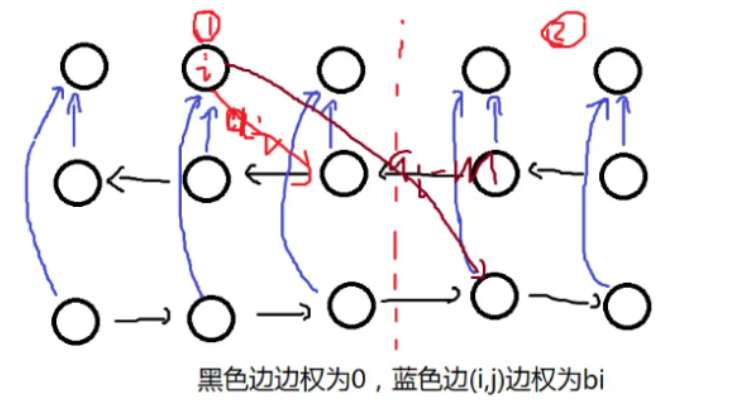
\includegraphics[scale=0.8]{优化建图1.png}        
        
        另外一个 \(trick\),棕边会是负权边,很明显不能使用 \(O(n*m)\)
        算法,可以这样去除负权边。
        
        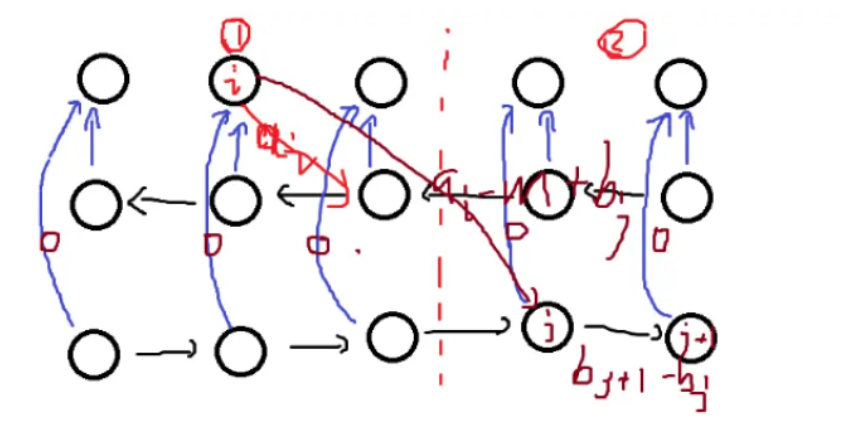
\includegraphics[scale=0.8]{优化建图2.png}      
        
        更改的地方在图中标出,前缀的黑边和蓝边没变化,主要变化是后缀的蓝边和黑边,这样棕边就为正数了。
        
        然后写一个dijkstra就可以,不能用拓扑排序求,因为不是 \(DAG\)。                
    \end{quote}
\end{itemize}

\begin{lstlisting}
// created on 25-5-1

// https://atcoder.jp/contests/abc232/tasks/abc232_g
const int N=1e6+10;
struct edge{ll v,w;};
struct Node{
	ll dis,w;
	bool operator>(const Node& a) const {
		return dis>a.dis;
	}
};
int n,m,ca[N],cb[N];
ll d[N],vis[N];
vector<edge> adj[N];
vector<pii> b(1);

void dijkstra() {
	priority_queue<Node,vector<Node>,greater<Node>>q;
	memset(d,63,sizeof d);
	q.push({0,1});
	d[1]=0;
	while (q.size()) {
		int u=q.top().w;
		q.pop();
		if (vis[u]) continue;
		vis[u]=1;
		for (auto ed : adj[u]) {
			ll v=ed.v,w=ed.w;
			if (d[v]>d[u]+w) {
				d[v]=d[u]+w;
				q.push({d[v],v});
			}
		}
	}
}

signed main(){
	scanf("%d%d",&n,&m);
	rep(i,1,n+1) scanf("%d",&ca[i]);	
	rep(i,1,n+1) {
		scanf("%d",&cb[i]);
		b.eb(cb[i],i);
	}
	sort(b.begin()+1,b.end(),[&](pii x,pii y){
		return x.fi<y.fi;
	});
	per(i,2,n+1) {
		int u=b[i].se+n,v=b[i-1].se+n;
		adj[u].eb(v,0);
	}
	rep(i,1,n) {
		int u=b[i].se+n*2,v=b[i+1].se+n*2;
		adj[u].eb(v,b[i+1].fi-b[i].fi);
	}
	rep(i,1,n+1) {
		int u=b[i].se;
		adj[u+n].eb(u,cb[u]),adj[u+n*2].eb(u,0);
		auto it=upper_bound(all(b),mp(m-ca[u]-1,(int)(1e9)));
		int tp=it-b.begin();
		if (tp<=n) adj[u].eb(b[tp].se+2*n,ca[u]+b[tp].fi-m);
		if (tp-1>=1) adj[u].eb(b[tp-1].se+n,ca[u]);
	}
	dijkstra();
	printf("%lld\n",d[n]);
}
\end{lstlisting}

\subsection{矩阵树定理}

\begin{itemize}
    \item 无权图
    \begin{quote}
        给出一个无向无权图, 设 $A$ 为邻接矩阵, $D$ 为度数矩阵(D[i][i] 为 i 的度数, 其他无值),
        则基尔霍夫矩阵为 $K = D - A$, 然后令 $K'$ 为 $K$ 去掉第 $k$ 行和第 $k$ 列的结果($k$ 任意),
        $det(K')$ 即为所求。       
    \end{quote}
    \item 有权图
    \begin{quote}
        设 $G$ 是一个带权无向连通图, 边权为 $w_{i,j}$, 其基尔霍夫矩阵 $K$ 定义为:
        度数矩阵 $D$ $-$ 邻接矩阵 $A$。然后也要变换为 $K'$ 并求 $det(K')$。\\
        
        度数矩阵 $D$: $D_{ii}$ 表示与顶点 $i$ 相连的边的权值和。 \\

        邻接矩阵 $A$: $A_{ij} = w_{ij}$ 仅当 $i$ 与 $j$ 之间有边。
    \end{quote}
\end{itemize}

\newpage

\fancyhead[L]{基础树论}
\section{基础树论}

\subsection{树的直径}

\noindent 树上任意一点,离他最远的点一定是直径两端的点之一。又称树的最长路径。

\begin{itemize}
\item 
任取一点 u, 从 u 向下搜, 同时返回收集边的权值, 记录两条路径 d1, d2。

\item 
d1: 记录从 u 点往下走的最长路径的长度。

\item
d2: 记录从 u 点往下走的次长路径的长度。

\item
对于每个点:ans = max({ans, d1 + d2})。
\end{itemize}

\begin{lstlisting}
// created on 24-8-24

int d1[N],d2[N],d;
void dfs(int u,int fa) {//reset d=0;
    d1[u]=d2[u]=0;
    for (auto v : adj[u]) {
        if (v==fa) continue;
        dfs(v,u);
        int t=d1[v]+1;
        if (t>d1[u]) d2[u]=d1[u],d1[u]=t;
        else if (t>d2[u]) d2[u]=t;
    }
        d=max(d,d1[u]+d2[u]);
}
\end{lstlisting}

\subsection{树的重心}

\noindent 选择树的某个点删除, 将树分为若干棵子树, 统计子树节点数并记录最大值。
取遍树上所有节点, 使最大值取到最小的节点被称为树的重心。

\noindent 性质:

\begin{itemize}
\item 树的重心如果不唯一, 至多存在两个, 且相邻。
\item 树的重心为根, 所有子树的大小不超过整颗树的大小的一半。
\item 树中所有点到某个点的距离和中, 到重心的距离和是最小的。
\item 把两棵树通过一条边相连得到一颗新的树, 新树的重心在连接两颗树的重心的路径上。
\item 在一颗树上添加或删除一个叶子, 重心最多只移动一条边的距离。
\end{itemize}

\begin{lstlisting}
// created on 24-8-24

//ctr 存重心
//sum 与 mxs 初始化为当前搜索子树的大小
int ctr,mxs,sz[N];
// mxs=1e9;
void getroot(int u,int fa) {
    sz[u]=1;
    int mss=0;
    for (auto v:e[u]) {   
        if (v==fa) continue;
        getroot(v,u);
        sz[u]+=sz[v];
        mss=max(mss,sz[v]);
    }
    mss=max(mss,n-sz[u]);
    if (mss<mxs) ctr=u,mxs=mss;
}
\end{lstlisting}

\subsection{树链剖分}

\noindent 变量名:

\begin{itemize}
    \item fa[u]: u 的父节点。
    \item dep[u]: u 的深度。
    \item son[u]: u 的重儿子。
    \item sz[u]: 存以 u 为根的子树节点数。
    \item top[u]: 存 u 所在重链的顶点。
    \item id[u]: 存 u 剖分后的新编号。
    \item nw[cnt]: 存新编号在树中所对应节点的权值。
\end{itemize}

\begin{lstlisting}
// created on 24-8-24

vector<int> e[N];
int fa[N],dep[N],son[N],sz[N];
int top[N];
//int id[N], nw[N], cnt;
void dfs1(int u, int f){
    fa[u] = f,dep[u] = dep[f] + 1,sz[u] = 1;
    for (auto x : e[u]){
        if (x == f) continue;
        dfs1(x, u);
        sz[u] += sz[x];
        if (sz[son[u]]<sz[x]) son[u]=x;
    }
}
void dfs2(int u, int t){
    top[u] = t;
    //id[u] = ++cnt,nw[cnt] = w[u];
    if (!son[u]) return;
    dfs2(son[u], t);
    for (int v : e[u]){
        if (v == fa[u] || v == son[u]) continue;
        dfs2(v, v);
    }
}
dfs1(root,-1);
dfs2(root,root);   
\end{lstlisting}

\subsection{最近公共祖先}

\noindent 基于树链剖分的最近公共祖先.

\begin{lstlisting}
// created on 24-8-24

int lca(int u, int v){
    while (top[u] != top[v]){
        if (dep[top[u]] < dep[top[v]]) swap(u,v);
        u = fa[top[u]];
    }
    return dep[u] < dep[v] ? u : v;
}
\end{lstlisting}

\noindent 基于倍增的最近公共祖先。

\begin{lstlisting}
// created on 24-8-24

VI e[N];
int dep[N], sz[N], fa[N][22];

void dfs(int x,int f){
    dep[x] = dep[f] + 1; 
    fa[x][0] = f, sz[x] = 1;
    for (int i = 1; i <= 20; i ++) {
        fa[x][i] = fa[fa[x][i - 1]][i - 1];
    }
    for (int y : e[x]) if (y != f) {
        dfs(y, x);
        sz[x] += sz[y];
    }
}
int lca(int x,int y) {
    if (dep[x] < dep[y]) swap(x, y);
    for (int i = 20; ~i; i --) {
        if (dep[fa[x][i]] >= dep[y]) x = fa[x][i];
    }
    if (x == y) return y;
    for (int i = 20; ~i; i --) {
        if (fa[x][i] != fa[y][i]) x = fa[x][i], y = fa[y][i];
    }
    return fa[x][0];
}   
\end{lstlisting}

\subsection{树上启发式合并}

\noindent 启发式合并作为一种思想,本质上还是把小的往大的里面合并。
\\

\noindent 统计答案时,先遍历轻儿子,算完一个儿子就要撤销其贡献。(如果需要撤销的话)
\\

\noindent 再扫重儿子,不撤销重儿子贡献,遍历轻儿子,加入其贡献,即可得到 u 的答案。

\begin{lstlisting}
// created on 24-8-24

// HDU 7435
const int N=5e5+10,M=1e6+10;
template<class T>
struct BIT {
    vector<T> c;
    int size;
    void init(int n) {
        this->size=n;
        c.assign(n,0);
    }
BIT(int n=0) {init(n); }
    T query(int x) { // 1 ... x
        //assert(x<=size);
        T s=0;
        for (;x;x-=x&(-x)) {
            s+=c[x];
        }
        return s;
    }
    void update(int x,T s) { // a[x] += s
        //assert(x != 0);
        for (;x<=size;x+=x&(-x)) {
            c[x]+=s;
        }
    }
};
BIT<unsigned long long> tr1(M);
BIT<unsigned long long> tr2(M);
BIT<unsigned long long> tr3(M);
VI e[N],nw;
ll a[N];
ll siz[N],dfn[N],st[N],ed[N],tot;
unsigned long long OvO[N];
unsigned long long res;
void dfs(int u,int f) { // 预处理出每个子树的大小,已经相应的dfs序
    siz[u]=1;
    st[u]=++tot;
    dfn[tot]=u;
    for (auto v : e[u]) if (v!=f) {
        dfs(v,u);
        siz[u]+=siz[v];
    }
    ed[u]=tot;
}
void calc(unsigned long long &val,int u) {
    // MAX * MAX - MAX * MIN
    // a[u] * (a[u] - a[v])
    unsigned long long q1=tr1.query(a[u]);
    unsigned long long q2=tr2.query(a[u]);
    unsigned long long v=(q1*a[u]*a[u])-q2*a[u];
    // a[v] * (a[v] - a[u])
    unsigned long long q4=tr2.query(M-10)-tr2.query(a[u]);
    unsigned long long q5=tr3.query(M-10)-tr3.query(a[u]);
    v+=q5-q4*a[u];
    val+=v*2;
}
void dsu(int u,int f,int okok) {
    int mx=-1,son=-1;
    for (auto v : e[u]) { // 处理出每个点的重儿子
        if (v!=f and siz[v]>mx) {
            mx=siz[v],son=v;
        }
    }
    for (auto v : e[u]) { // 算出每个轻儿子的答案
        if (v==f or v==son) continue;
        dsu(v,u,0); // okok 为零代表会清空相应的答案
        OvO[u]+=OvO[v]; // 题目要求
    }
    if (son!=-1) dsu(son,u,1),OvO[u]+=OvO[son];
    // 计算重儿子,重儿子的答案不清除
    for (auto v : e[u]) {
        if (v!=f and v!=son) {
            for (int i=st[v];i<=ed[v];i++) {
                // 算每个轻儿子子树在与其他子树上面的答案
                int x=dfn[i];
                calc(OvO[u],x);
            }
            for (int i=st[v];i<=ed[v];i++) {
                // 更新
                int x=dfn[i];
                tr1.update(a[x],1);
                tr2.update(a[x],a[x]);
                tr3.update(a[x],a[x]*a[x]);
                nw.pb(x);
            }
        }
    }
    // 计算父节点的答案
    calc(OvO[u],u);
    tr1.update(a[u],1);
    tr2.update(a[u],a[u]);
    tr3.update(a[u],a[u]*a[u]);
    nw.pb(u);
    if (okok==0) { // 如果检查标记为假就清除一下数组啥的
        for (auto v:nw) {
            tr1.update(a[v],-1);
            tr2.update(a[v],-a[v]);
            tr3.update(a[v],-a[v]*a[v]);
        }
        nw.clear();
    }
    // cout<<u<<" "<<OvO[u]<<endl;
    res^=OvO[u];
}
void solve() {
    int n; Read(n);
    rep(i,1,n) {int x,y;
        Read(x);
        Read(y);
        e[x].pb(y);
        e[y].pb(x);
    }
    rep(i,1,n+1) Read(a[i]);
    dfs(1,0);
    dsu(1,0,0);
    cout<<res;
}
signed main(){
    solve();
    return 0;
}
\end{lstlisting}

\subsection{基环树}

\noindent 基环树定义为正常的树加上一条边构成一个环,即 $n$ 个节点 $n$ 条边的无向联通图。\\
当然这只是一个比较泛的定义,具体情况具体分析。

\subsubsection{基环树找环}

\begin{lstlisting}
// created on 25-5-2

ll dep[N],fa[N],ok[N];
vl e[N],loop;

void getloop(ll u) {
    dep[u]=dep[fa[u]]+1;
    for (auto v : e[u]) {
        if (v==fa[u]) continue;
        if (!dep[v]) {
            fa[v]=u;
            getloop(v);
        } else if (dep[v]<dep[u]) {
            for (int i=u;;i=fa[i]) {
                ok[i]=1;
                loop.pb(i);
                if (i==v) break;
            }
        }
    }
}   
\end{lstlisting}

\subsubsection{基环树DP}

\noindent P2607 骑士:

\begin{itemize}
\item 题意:每个人有一个不可以同时上场的人,每个人都有一个权值,求最大。
\item 思路:
\begin{enumerate}
\item 由于不保证图联通,这个图可能会是一个基环树森林。
\item 对于每棵基环树,先断开环上的任意一条边,然后对两个端点都做一次树形DP,两次答案求最大值即可。
\item 累加每一颗集环树的最大值即可。
\end{enumerate}
\item 细节:
\begin{enumerate}
\item 事实证明存无向图是完全没有必要的,因为本身有向图就携带着指向上一个节点的信息,
而且这个信息更利于维护我们删边之后的操作。
\item 每个联通块内有且只有一个简单环,这样我们考虑把每个联通块的环上删一条边,这样它必然构成树。
\item 存一下每个人不能同时上场的人为他的父亲,强制不选它的父亲对它进行DP,
强制不选它对它的父亲进行DP,然后取一个最大值即可。
\end{enumerate}
\end{itemize}

\begin{quote}
    在处理基环树问题时,首先需要找到构成环的边。
    这可以通过深度优先搜索(DFS)实现,通过记录节点的前驱和访问状态来检测环。如果在搜索过程中遇到一个已经访问过的节点,那么这个节点及其前驱节点就在环上。
    找到环后,可以选择环上的任意两个节点,断开它们之间的边,然后分别以这两个节点为根进行动态规划。这样,原问题就转化为了两个独立的树形动态规划问题。
\end{quote}

\begin{lstlisting}
// created on 25-5-20 

const int N=1E6+10;
int n,r1,r2;
ll val[N],vis[N];
ll f[N][2];
vi e[N];

void find(int u,int rt) {
	vis[u]=1;
	for (auto v:e[u]) {
		if (v==rt) {
			r1=u,r2=v;
			return;
		}
		if (vis[v]) continue;
		find(v,rt);
	}
	return;
}

ll dfs(int u,int rt) {
	f[u][0]=0;
	f[u][1]=val[u];
	for (auto v:e[u]) {
		if (v==rt) continue;
		dfs(v,rt);
		f[u][0]+=max(f[v][0],f[v][1]);
		f[u][1]+=f[v][0];
	}
	return f[u][0];
}

void solve(int testid) {
	cin>>n;
	rep(i,1,n+1) {
		ll v,x;
		cin>>x;
		e[x].pb(i);
		val[i]=v;
	}
	ll ans=0;
	ll ok=0;
	rep(i,1,n+1) {
		if (vis[i]) continue;
		r1=r2=0;
		find(i,i);
		ll res1=dfs(r1,r1);
		ll res2=dfs(r2,r2);
		ans+=max(res1,res2);
	}
	cout<<ans<<endl;
}      
\end{lstlisting}

\subsection{树上拓扑序计数}

\begin{itemize}
\item 定义
树本身就是一种有向无环图,可以计算一棵树有多少个不同的拓扑序列。
\item 求法
跑一遍树形 $dp$,时间复杂度 $O(n)$,$dp[x]=(\prod dp[son]) \frac{(sz[x]-1)!}{\prod (sz[son]!)}$。

也能这样算,$n! \times \prod_{i=1}^{n} \frac{1}{sz[i]}$。
\item 用法
这个可以抽象到一些问题上去,如:一堆点和一个排列, 给出每个点的大小关系,求对应的方案数。
我们可以按大小关系建一颗树,然后求这棵树有多少个拓扑序列。
\end{itemize}

\subsection{虚树}

\noindent 抽离查询点和它们两两之间的最近公共祖先以及树根构成的树,构成虚树的点:查询点+两两的最近公共祖
先+树根。
\\

\noindent 通常是解决一类树形dp的优化方式,通常是计算树上部分信息,但是询问点又有限,构建虚数缩小查询规
模。

\begin{lstlisting}
// created on 24-8-24

// CF613
// 给定一颗 n 个点的树, 有 q 组询问
// 每次询问给定 k 个点, 你可以删掉不同于这 k 个点的一些点, 使得这些点两两不连通.
// 求最小删掉多少点, 如果不可能则输出 -1, 询问独立.
const int N=1e5+10;
int n,m,q,tot,ans,dfn[N],dep[N],fa[N][22],dp[N];
int cur[N];
// e[N] 为原树图, tmp 为虚树图
vector<int> e[N],tmp[N];
// 预处理dfs序以及倍增lca
void dfs_init(int u,int f) {
    dfn[u]=++tot;
    dep[u]=dep[f]+1,fa[u][0]=f;
    for (int uu=1;uu<=20;uu++)
    fa[u][uu]=fa[fa[u][uu-1]][uu-1];
    for (auto y:e[u]) if (y!=f) {
        dfs_init(y,u);
    }
}
int lca(int x,int y) {
    if (dep[x]<dep[y]) swap(x,y);
    for (int uu=20;~uu;uu--) {
        if (dep[fa[x][uu]]>=dep[y]) x=fa[x][uu];
    }
    if (x==y) return y;
    for (int uu=20;~uu;uu--) {
        if (fa[x][uu]!=fa[y][uu]) x=fa[x][uu],y=fa[y][uu];
    }
    return fa[x][0];
}
// 建立虚树
void build_vtree() {
    // 手写栈
    static int s[N],top=0;
    // 把查询点按dfs序排好
    sort(cur+1,cur+m+1,[&](int a,int b) {
        return dfn[a]<dfn[b];
    });
    // 随便搞得树根,树根入栈
    s[top=1]=1;
    // 如果树根也是查询点,就不把树根二次入栈
    if (cur[1]!=1) s[++top]=cur[1];
    rep(uu,2,m+1) {
        int l=lca(s[top],cur[uu]);
        // cur[uu] 不是 s[top] 子树里面的节点
        // lca 下面的路径上的关键点都应该出栈, 出栈时连单向边.
        while (top>1&&dep[s[top-1]]>=dep[l])
        tmp[s[top-1]].eb(s[top]),top--;
        // 说明 lca 不在栈中
        // 应该先把 s[top] 与 lca 相连, 再把 lca 和 cur[uu] 入栈
        if (l!=s[top]) tmp[l].eb(s[top]),s[top]=l;
        s[++top]=cur[uu];
    }
    // 对最后一条边连边出栈
    while (top) tmp[s[top-1]].eb(s[top]),top--;
}
// 题目要求的树形dp
void dfs(int x) {
    if (dp[x]) {
        for (auto y:tmp[x]) {
            dfs(y);
            if (dp[y]) ans++,dp[y]=0;
        }
    } else {
        for (auto y:tmp[x]) {
            dfs(y);
            dp[x]+=dp[y],dp[y]=0;
        }
        if (dp[x]>1) ans++,dp[x]=0;
    }
    // 注意的是要在这里把边都删了
    tmp[x].clear();
}
signed main(){
    scanf("%d",&n);
    int u,v;
    rep(uu,1,n) {
        scanf("%d%d",&u,&v);
        e[u].eb(v);
        e[v].eb(u);
    }
    dfs_init(1,0);
    scanf("%d",&q);
    while (q--) {
        scanf("%d",&m);
        // 记得把拟定的树根的信息重置
        cnt=ans=dp[1]=0;
        rep(uu,1,m+1) {
            scanf("%d",&cur[uu]);
            dp[cur[uu]]=1;
        }
        bool ok=1;
        for (int uu=1;uu<=m;uu++) {
            if (dp[fa[cur[uu]][0]]) ok=0;
        }
        if (!ok) {
            rep(uu,1,m+1) dp[cur[uu]]=0;
            puts("-1");
            continue;
        }
        build_vtree();
        dfs(1);
        printf("%d\n",ans);
        rep(uu,1,m+1) dp[cur[uu]]=0;
    }
    return 0;
}    
\end{lstlisting}

\subsection{prufer 序列}

\noindent \(prufer\) 序列可以将一颗 \(n\) 个点的树映射到一个长度为 \(n - 2\) 的序列上,并将其从树上删除,直到树上
只剩两个节点。
\\

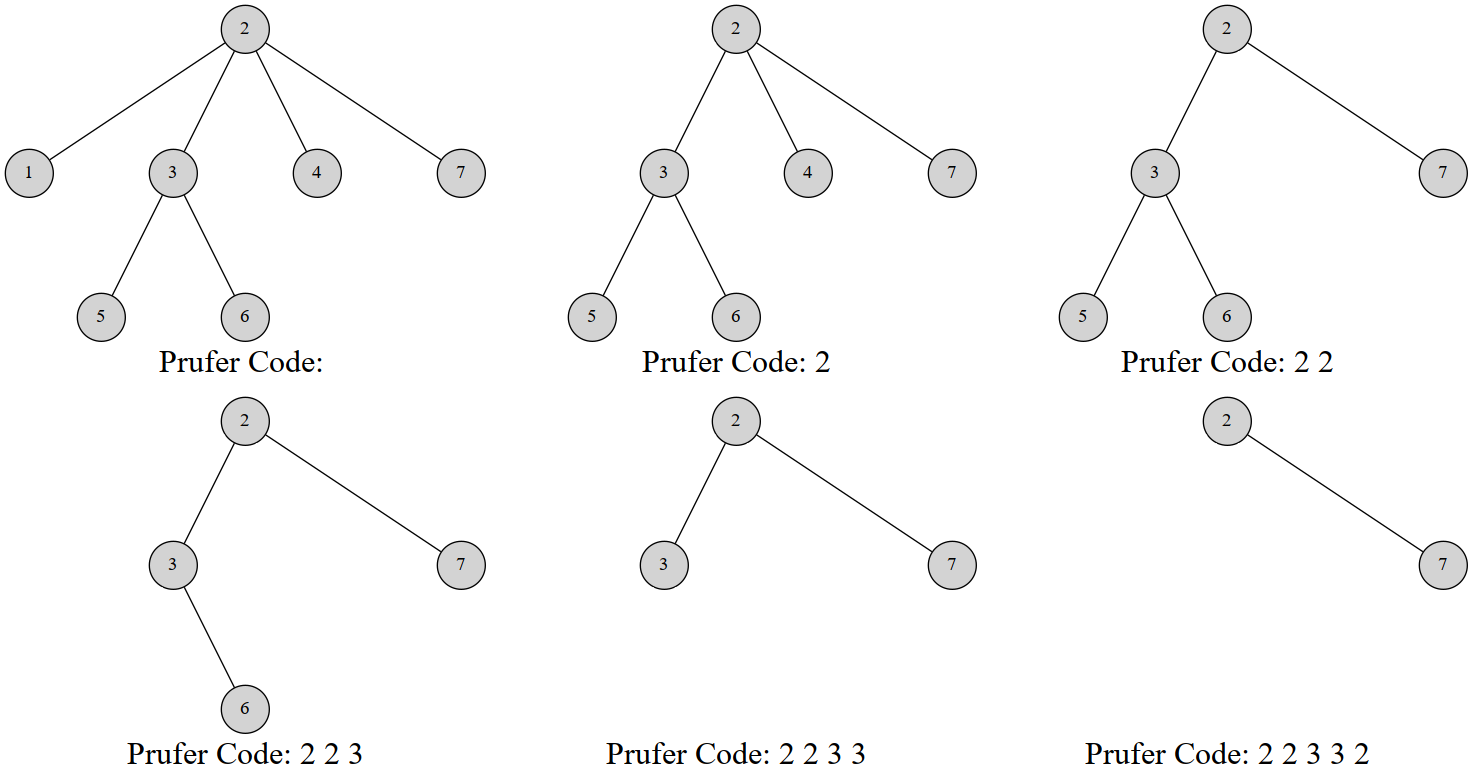
\includegraphics[scale=0.3]{prufer1.png}

\noindent 两棵树不相同的时候, 它们的 \(prufer\) 序列不一样。

\begin{itemize}
\item 构造过程: 每次找到编号最小的一个叶子节点,将与其连接的那个点加入序列,并将其在树上删
除,直到树上只有两个节点。

\item 序列性质: 
\begin{itemize}
    \item 树中最后剩下的两个点中,一定会有一个节点是编号最大的 \(n\) 点。
    \item 每个节点在序列中出现的次数为这个点的度数 \(-1\)。
    \item 给定度数为 \(d_1 \cdots d_n\) 的一棵无根树共有 \(\frac{(n-2)!}{\prod_{i=1}^{n} (d_i - 1)!}\)。
\end{itemize}

\item 证明过程:
在构造序列时,每次将与编号最小的叶子节点加入到序列中,而编号最小的叶子节点是
很容易根据 \(prufer\) 序列求出的,因此序列中的每个数表示的不是一个点而是一条边,这样就有了 \(n-2\)
条边,而最后一条边显然是与 \(n\) 号节点相连的。以上,\(prufer\) 序列就表示出了 \(n-1\) 条
边,也就唯一表示出了一棵树。
\end{itemize}

\begin{lstlisting}
// created on 24-8-23

vector<VI> adj;
VI parent;
void dfs(int u) {
    for (auto v : adj[u]) {
        if (v!=parent[u]) {
            parent[v]=u;
            dfs(v);
        }
    }
}
vector<int> prufer_code() {
    int n=adj.size(),ptr=-1;
    parent.resize(n),parent[n-1]=-1;
    dfs(n-1);
    vector<int> degree(n);
    for (int i=0;i<n;i++) {
        degree[i]=adj[i].size();
        if (degree[i]==1 and ptr==-1) {
            ptr=i;
        }
    }
    vector<int> code(n-2);
    int leaf=ptr;
    for (int i=0;i<n-2;i++) {
        int next=parent[leaf];
        code[i]=next;
        if (--degree[next]==1 and next<ptr) {
            leaf=next;
        }
        else {
            ptr++;
            while (degree[ptr]!=1) {
                ptr++;
            }
            leaf=ptr;
        }
    }
    return code;
}
vector<pair<int,int>> prufer_decode(vector<int> const& code) {
    int n=code.size()+2;
    vector<int> degree(n,1);
    for (int i:code) degree[i]++;
    int ptr=0;
    while (degree[ptr]!=1) ptr++;
    int leaf=ptr;
    vector<pair<int,int>> edges;
    for (int v : code) {
        edges.emplace_back(leaf,v);
        if (--degree[v]==1 and v<ptr) {
            leaf=v;
        }
        else {
            ptr++;
            while (degree[ptr]!=1) ptr++;
            leaf=ptr;
        }
    }
    edges.emplace_back(leaf,n-1);
    return edges;
}
\end{lstlisting}

\newpage

\fancyhead[L]{基础动态规划}
\section{基础动态规划}

\subsection{01 背包}

\begin{lstlisting}
// created on 24-8-24

for (int i = 1; i <= n; i ++)
    for (int j = m; j >= v[i]; j --)
        f[j] = max(f[j], f[j - v[i]] + w[i]);
cout << f[m] << endl;    
\end{lstlisting}

\subsection{完全背包}

\noindent 完全背包模型与 0-1 背包类似,
与 0-1 背包的区别仅在于一个物品可以选取无限次,而非仅能选取一次。

\noindent 可以考虑一个朴素的做法:对于第 \( i \) 件物品,枚举其选了多少个来转移。
这样做的时间复杂度是 \( O(n^3) \) 的。
\\

\noindent 状态转移方程如下:
\(f_{i,j} = \max_{k=0}^{+\infty} (f_{i-1,j-k \times w_i} + v_i \times k)\)
考虑做一个简单的优化。可以发现,对于 \( f_{i,j} \),只要通过 \( f_{i,j-w_i} \) 转移就可以了。因此状态转移方程为:
\(f_{i,j} = \max(f_{i-1,j}, f_{i,j-w_i} + v_i)\)


\noindent 理由是当我们这样转移时,\( f_{i,j-w_i} \) 已经由 \( f_{i,j-2 \times w_i} \) 更新过,
那么 \( f_{i,j-w_i} \) 就是充分考虑了第 \( i \) 件物品所选次数后得到的最优结果。
换言之,我们通过局部最优子结构的性质重复使用了之前的枚举过程,优化了枚举的复杂度。

\begin{lstlisting}
// created on 24-8-24

for (int i = 1; i <= n; i ++ )
    for (int j = v[i]; j <= m; j ++ )
        f[j] = max(f[j], f[j - v[i]] + w[i]);
cout << f[m] << endl;    
\end{lstlisting}

\subsection{多重背包}

\noindent 多重背包也是 0-1 背包的一个变式。
与 0-1 背包的区别在于每种物品有 \(k_i\) 个,而非一个。
\\


\begin{lstlisting}
// created on 24-8-24

// 二进制分组
// 定义int变量cnt=0,int数组f,w,v
for (int i = 1; i <= n; i ++){
    int a, b, s; 
    cin >> a >> b >> s;
    int k = 1;
    while (k <= s){
        cnt ++;
        v[cnt] = a * k, w[cnt] = b * k;
        s -= k, k *= 2;
    }
    if (s > 0){
        cnt ++;
        v[cnt] = a * s, w[cnt] = b * s;
    }
}
n = cnt;
for (int i = 1; i <= n; i ++ )
    for (int j = m; j >= v[i]; j -- )
        f[j] = max(f[j], f[j - v[i]] + w[i]);
cout << f[m] << endl;    
\end{lstlisting}

\subsection{分组背包}

\begin{lstlisting}
// created on 24-8-24

for (int k = 1; k <= ts; k++) // 循环每一组
    for (int i = m; i >= 0; i--) // 循环背包容量,倒序遍历
        for (int j = 1; j <= cnt[k]; j++) // 循环该组的每一个物品
            if (i >= w[t[k][j]]) // 背包容量充足
                dp[i] = max(dp[i], dp[i - w[t[k][j]]] + c[t[k][j]]); // 像0-1背包一样状态转移
\end{lstlisting}

\subsection{二维费用的背包}

\noindent 有 \(n\) 件物品和一个容量为 \(w\) 的背包,背包能承受的最大重量为 \(m\),
每件物品只能用一次,第 \(i\) 件物品
的体积是 \(w_i\),重量是 \(m_i\),价值是 \(v_i\),求解在满足制约的情况下总价值最大。
\\

\noindent 思路:背包的限制条件由一个变成两个,那么循环多一维即可。

\begin{lstlisting}
// created on 24-8-23

for (int i = 1; i <= n; i++)
    for (int j = W; j >= w; j--) //容量限制
        for (int k = M; k >= m; k--) //重量限制
            dp[j][k] = max(dp[j][k], dp[j - w][k - m] + v);    
\end{lstlisting}

\subsection{树上背包}

\noindent 有一些树形 dp 问题可以抽象为背包问题, 可以建模为 "分组背包", 具体如下:

\begin{itemize}
\item 分组。根节点 \(u\) 的每一个子树是一个分组。
\item 背包的容量。把以 \(u\) 为根的整棵树上的树枝看出背包容量。
\item 物品。把每个数字看做一个物品, 体积为 1, 树枝上的物品数量看作价值.
\item 背包目标。能放入背包的总价值最大, 就是留在树枝上的苹果数最多。
\end{itemize}

\begin{lstlisting}
// created on 24-8-23

for (int i = 0; i < edge[i].size(); i ++ ) { // 把 u 的每一个子树看作一个分组
    ....
    for (int j = sum[u]; j >= 0; j --) {  // u 的树枝总量看成背包容量
        for (int k = 0; k <= j - 1; k ++ ) { // 用 k 变量该组的所有方案
            dp[u][j] = max(dp[u][j], dp[u][j-k-1] + dp[v][k] + w);
        }
    }
}
\end{lstlisting}

\subsection{单调队列优化 DP}

\noindent 一般都是维护一个双端队列, 从前端弹出元素保证约束, 后端弹出元素保证单调增/减。
\\

\noindent 模版题为 P2034, 给出 \(n\) 个数字的数组, 
选取若干个数, 不能同时选取 \(k\) 个连续的数字, 求能选取的最大值。
\\ 

\noindent 这里明显是把附近 \(k\) 个位置的, 单调丢到队列中维护。

\begin{lstlisting}
// created on 25-5-23

int n,k;

void solve(int testid) {
	cin>>n>>k;
	vector<vl> f(n+1,vl(2));
	vl a(n+1),sa(n+1);
	rep(i,1,n+1) {
		cin>>a[i];
		sa[i]=sa[i-1]+a[i];
	}
	deque<pair<ll,ll>> q{mp(0,0)};
	rep(i,1,n+1) {
		f[i][0]=max(f[i-1][0],f[i-1][1]);
		while (SZ(q)&&q.front().se<i-k) q.pop_front();
		f[i][1]=q.front().fi+sa[i];
		while (SZ(q)&&f[i][0]-sa[i]>=q.back().fi) q.pop_back();
		q.push_back(mp(f[i][0]-sa[i],i));
	}
	cout<<max(f[n][1],f[n][0]);
} 
\end{lstlisting}

\subsection{数位 DP}

\noindent 记忆化搜索数位 \(DP\)。

\begin{itemize}
\item 
题意

我们定义一个数为蛇数当且仅当最高位的数位大于其他所有的数位。
给范围 \(L,R\) 求范围内存在多少蛇数。
\end{itemize}

\noindent 数位 \(DP\) 需要考虑 前导零对问题有没有影响,
以及所有的数位 \(DP\) 要考虑 \(lim\) 的约束, 这里前导零对答案有影响在状态栏用 \(lead\) 来表示,
这道题对蛇数的定义是 \(>9\) 的数 但是为了方便假定 \(<=9\) 的数全是蛇数。

\begin{lstlisting}
// created on 25-5-2

ll a[100];
ll f[100][2][2][10];

ll dfs(ll u,ll lim,ll lead,ll val) {
    if (lead) val=0; // 如果存在前导零
    if (!u) return 1; // 设置边界
    if (~f[u][lim][lead][val]) return f[u][lim][lead][val];
    ll up=lim?a[u]:9,ans=0; // 这里不超过 x 的上限最大可以是多少
    // 如果不存在前导零了
    // 根据题目意思这个数会是最大的数 
    // up 变量需要根据题目条件在进行约束
    if (!lead) up=min(up,val-1);
    for (int i=0;i<=up;i++) {
        ans+=dfs(u-1,lim&&(i==a[u]),lead&&(i==0),lead?i:val); 
    }
    f[u][lim][lead][val]=ans;
    return ans;
}

ll get(ll x) {
    memset(f,-1,sizeof(f));
    ll len=0;
    while (x) {
        a[++len]=x%10;
        x/=10;
    }
    return dfs(len,1,1,0);
}

signed main() {
    ll l,r;
    cin>>l>>r;
    cout<<get(r)-get(l-1)<<endl;	
}    
\end{lstlisting}

\newpage

\fancyhead[L]{博弈论}
\section{博弈论}

\noindent 大概下面所有的 $k$ 都代表自然数。

\subsection{Bash 博弈}

\begin{itemize}
    \item 游戏设定:
    \begin{itemize}
        \item 有一堆 $n$ 个物品, 两个人轮流从这里面取东西。
        \item 每次最少取一个东西, 最多取 m 个物品。
    \end{itemize}
    
    \item 必胜条件:
    \begin{itemize}
        \item 最后取光者胜, 当 $n \% (m + 1) == 0$ 时, 后手必胜, 否则先手必胜。
        \item 最后取光者输, 当 $n = (m + 1) * k + 1$ 时, 后手必胜, 否则先手必胜。
    \end{itemize}
\end{itemize}

\subsection{EX Bash 博弈}

\begin{itemize}
    \item 游戏设定:
    \begin{itemize}
        \item 有一堆 $n$ 个物品, 两个人轮流从这里面取东西。
        \item 每人可以取走 $x$ 个石子($a \leq x \leq b$)。
        \item 若最后剩余物品的个数小于 $a$ 个, 则不能再取。
        \item 拿到最后一颗石头者获胜。
    \end{itemize}
    
    \item 必胜条件:
    \begin{itemize}
        \item $n = k * (a + b)$ 时, 后手必胜。
        \item $n = k * (a + b) + R_1$ ($0 \leq R_1 < a$) 时, 后手必胜。
        \item $n = k * (a + b) + R_2$ ($a \leq R_2 \leq b$) 时, 先手必胜。
        \item $n = k * (a + b) + R_3$ ($b < R_3 < a + b$) 时, 先手必胜。
    \end{itemize}
\end{itemize}

\subsection{Nim 博弈}

\begin{itemize}
    \item 游戏设定:
    \begin{itemize}
        \item  有 $n$ 堆石头, 给出每一堆的石头数量。
        \item  两名玩家轮流行动, 每人每次任选一堆。
        \item 拿走正整数颗石头, 拿到最后一颗石头的人获胜。
        \item 几个特点: 不能跨堆拿, 不能不拿石子。
    \end{itemize}
    
    \item 必胜条件:
    \begin{quote}
        记初始情况下各堆石子的数量 ($A_1,A_2,A_3,...,A_n$), 
        定义尼姆和为 $Sum_N = A_1 \bigoplus A_2 \bigoplus A_3 \bigoplus ... \bigoplus A_n$。 
        当 $Sum_N = 0$ 时先手必败, 反之先手必胜。  \\
        
        胜利的策略就是在取走棋子后,使尼姆和为0。
        只要取走棋子前,尼姆和不为0,一定有办法取走部分棋子使尼姆和为0。
        另一个游戏者无论怎么拿,取走棋子后尼姆和都不会为0。
        以此策略,只要在取棋子时照策略进行,一定会胜利。
    \end{quote}

    \item 具体取法:
    \begin{quote}
        具体取法为先计算尼姆和, 在对每一堆石子计算 $A_i \bigoplus Sum_N$, 记为 $X_i$。
        若得到的值 $X_i < A_i$, $X_i$ 即为一个可行解, 即剩下 $X_i$ 颗石头, 取走 $A_i - X_i$ 颗石头。
        (这里是小于号因为至少要取走一颗石头)。        
    \end{quote}
\end{itemize}

\subsection{Nim-K 游戏}

\begin{itemize}
    \item 游戏设定:
    \begin{itemize}
        \item $N$ 堆石子,每堆有若干石子。
        \item 玩家轮流操作,每次选择不超过 $K$ 堆。
        \item 对每堆取走\textbf{不同}的正整数颗石子。
        \item 取最后一颗石子者获胜。
    \end{itemize}
    
    \item 必胜条件:
    \begin{itemize}
        \item 将每堆石子数表示为二进制。
        \item 定义 $One_i$ 为第 $i$ 位上 $1$ 的总数。
        \item 若对于每一位 $i$,$One_i \not\equiv 0 \pmod{K+1}$。
        \item 则先手有必胜策略。
    \end{itemize}
\end{itemize}

\subsection{Anti-Nim 游戏}

\begin{itemize}
    \item 游戏设定:
    \begin{itemize}
        \item $N$ 堆石子。
        \item 玩家轮流操作,每次选择一堆取走正整数颗石子。
        \item 取最后一颗石子者\textbf{出局}。
    \end{itemize}
    
    \item 必胜条件:
    \begin{itemize}
        \item 情况1:所有堆石子数 $\leq 1$ 且总数为偶数。
        \item 情况2:至少一堆石子数 $>1$ 且总数 $\neq 0$。
        \item 满足上述任一条件则先手有必胜策略。
    \end{itemize}
\end{itemize}

\subsection{阶梯-Nim} 

\begin{itemize}
    \item 游戏设定:
    \begin{itemize}
        \item $N$ 级台阶,每级有若干石子。
        \item 玩家轮流操作,选择一级台阶取石子。
        \item 将取下的石子移到下一级台阶。
        \item 地面上的石子不可再移动。
        \item 取最后一颗石子者获胜。
    \end{itemize}
    
    \item 必胜策略:
    \begin{itemize}
        \item 仅对\textbf{奇数级}台阶做传统Nim博弈。
        \item 计算奇数级石子数的异或和 $Sum_N$。
        \item 若 $Sum_N = 0$ 则先手必败。
        \item 否则先手必胜。
    \end{itemize}
\end{itemize}

\subsection{SG游戏(有向图游戏)}

\begin{itemize}
    \item 基本定义:
    \begin{itemize}
        \item 使用SG值表示局面状态:
        \begin{itemize}
            \item $0$:必败态
            \item 非$0$:存在必胜策略
        \end{itemize}
        \item 终态SG值根据游戏规则手动设定
    \end{itemize}
    
    \item 计算方法:
    \begin{itemize}
        \item 非终态节点的SG值:
        \begin{quote}
        \( SG(u) = \text{mex}\{SG(v) \mid u \to v\} \)。
        (mex表示最小未出现的非负整数)
        \end{quote}
        \item 单游戏胜负判定:
        \begin{itemize}
            \item 根节点SG值为$0$:先手必败。
            \item 根节点SG值非$0$:先手必胜。
        \end{itemize}
        \item 多游戏组合:
        \( SG_{total} = \bigoplus_{i=1}^n SG_i \)(异或和)
    \end{itemize}
    
    \item 复杂度:
    \begin{itemize}
        \item 使用哈希表存储可达状态。
        \item 时间复杂度:$O(N + M)$($N$为状态数,$M$为转移数)。
    \end{itemize}
\end{itemize}

\begin{lstlisting}
// created on 24-8-24

int n, m, a[N], num[N];
int sg(int x) {
    if (num[x] != -1) return num[x];
    unordered_set<int> S;    
    for (int i = 1; i <= m; ++ i) {
        if(x >= a[i]) {
            S.insert(sg(x - a[i]));
        }
    }
    for (int i = 0; ; ++ i) {
        if (S.count(i) == 0) {
            return num[x] = i;            
        }
    }
}
void Solve() {
    cin >> m;
    for (int i = 1; i <= m; ++ i) cin >> a[i];
    cin >> n;
    int ans = 0; 
    memset(num, -1, sizeof num);
    for (int i = 1; i <= n; ++ i) {
        int x; cin >> x;
        ans ^= sg(x);
    }
    if (ans == 0) no;
    else yes;
}
\end{lstlisting}

\subsection{Anti-SG 游戏}

\begin{itemize}
    \item \textbf{游戏规则}:
    \begin{itemize}
        \item 采用标准SG游戏的规则。
        \item \textbf{胜负判定反转}:最先无法行动的一方获胜。
    \end{itemize}
    
    \item \textbf{必胜条件}:
    \begin{itemize}
        \item 情况1:
        \begin{itemize}
            \item 所有单局游戏的SG值 $\leq 1$。
            \item 且总SG值 $= 0$(即各局SG值的异或和为零)。
        \end{itemize}
        
        \item 情况2:
        \begin{itemize}
            \item 至少存在一局游戏的SG值 $> 1$。
            \item 且总SG值 $\neq 0$。
        \end{itemize}
    \end{itemize}
    
    \item \textbf{本质}:与Anti-Nim游戏的结论一致。
\end{itemize}

\subsection{Multi-SG 游戏}

\begin{itemize}
    \item \textbf{游戏设定}:
    \begin{itemize}
        \item $N$ 堆石子,每堆有若干石子。
        \item 玩家可选两种操作:
        \begin{itemize}
            \item 任选一堆,取走正整数颗石子(至少取1颗)。
            \item 任选一堆(石子数 $> 2$),将其分裂为两堆非空石子。
        \end{itemize}
        \item 取最后一颗石子者获胜。
    \end{itemize}
    
    \item \textbf{SG函数定义}:
    \begin{quote}
        \[ 
            SG(x) =
            \begin{cases} 
            x - 1, & x \equiv 0 \pmod{4} \\
            x,     & x \equiv 1 \pmod{4} \\
            x,     & x \equiv 2 \pmod{4} \\
            x + 1, & x \equiv 3 \pmod{4}
            \end{cases}
        \]
    \end{quote}
    
    \item \textbf{胜负判定}:
    \begin{itemize}
        \item 计算所有堆的SG值异或和:
        \( SG_{total} = \bigoplus_{i=1}^N SG(x_i) \)。
        \item 若 $SG_{total} \neq 0$,先手有必胜策略。
        \item 否则先手必败。
    \end{itemize}
\end{itemize}

\subsection{Every-SG 游戏}

\begin{itemize}
    \item \textbf{游戏设定}:
    \begin{itemize}
        \item 给定一个有向无环图(DAG)。
        \item $K$ 个顶点上放置了石子。
        \item 玩家轮流操作,必须移动\textbf{所有}还能移动的石子。
        \item 无法操作的一方出局。
    \end{itemize}
    
    \item \textbf{关键定义}:
    \begin{itemize}
        \item 对于每个子游戏,定义$\text{step}$为游戏结束所需的最大回合数。
    \end{itemize}
    
    \item \textbf{必胜条件}:
    \begin{itemize}
        \item 若存在某个子游戏的$\text{step}$为奇数。
        \item 则先手有必胜策略。
    \end{itemize}
\end{itemize}

\subsection{威佐夫博弈}

\begin{itemize}
    \item \textbf{游戏设定}:
    \begin{itemize}
        \item 两堆石子,数量分别为$(a, b)$。
        \item 玩家可选操作:
        \begin{itemize}
            \item 任选一堆取任意正整数颗。
            \item 同时从两堆取相同数量颗(至少取1颗)。
        \end{itemize}
        \item 取最后一颗石子者获胜。
    \end{itemize}
    
    \item \textbf{必败态(P-positions)}:
    \begin{itemize}
        \item 前几项:$(1,2),\ (3,5),\ (4,7),\ (6,10),\ \ldots$。
        \item 模式:
        \begin{itemize}
            \item 每对第一个数是之前未出现的最小整数。
            \item 第二个数 $= \text{第一个数} + k$($k$为对序号)。
        \end{itemize}
    \end{itemize}
    
    \item \textbf{通项公式}:
    \(
    \text{First}_k = \left\lfloor k\phi \right\rfloor, \quad 
    \text{Second}_k = \left\lfloor k\phi^2 \right\rfloor
    \)
    其中$\phi = \frac{1+\sqrt{5}}{2}$(黄金比例)。
    
    \item \textbf{高精度处理}:
    \begin{itemize}
        \item 当石子数 $> 10^9$ 时:
        \(
        \phi \approx 1.618033988749894848204586834
        \)
        \item 可直接使用此近似值计算。
    \end{itemize}
\end{itemize}

\begin{lstlisting}
// created on 24-8-23

const double lorry = (sqrt(5.0) + 1.0) / 2.0;
//const double lorry = 1.618033988749894848204586834;

void Solve() {
    int n, m; cin >> n >> m;
    if (n < m) swap(n, m);
    double x = n - m;
    if ((int)(lorry * x) == m) cout << "lose\n";
    else cout << "win\n";
}
\end{lstlisting}

\subsection{斐波那契博弈}

\begin{itemize}
    \item \textbf{游戏设定}:
    \begin{itemize}
        \item 初始一堆石子,数量为 $N$。
        \item 玩家轮流取石子,规则:
        \begin{itemize}
            \item 先手第一次可取任意数量(至少取1颗,但不能取完)。
            \item 后续每次取的数量不超过对手上次取的数量的2倍。
            \item 取最后一颗石子者获胜。
        \end{itemize}
    \end{itemize}
    
    \item \textbf{必胜条件}:
    \begin{itemize}
        \item 设$F_k$表示第$k$个斐波那契数($F_1=1, F_2=2, F_3=3, F_4=5, \ldots$)。
        \item 当且仅当$N$是斐波那契数时(即$\exists k\ F_k = N$)。
        \item 先手处于必败态。
        \item 否则先手有必胜策略。
    \end{itemize}
    
    \item \textbf{数学背景}:
    \begin{itemize}
        \item 基于Zeckendorf定理:任何正整数可唯一表示为不相邻的斐波那契数之和。
        \item 最优策略涉及保持游戏状态始终为非斐波那契数。
    \end{itemize}
\end{itemize}

\subsection{树上删边游戏}

\begin{itemize}
    \item \textbf{游戏设定}:
    \begin{itemize}
        \item $N$个节点的有根树。
        \item 玩家轮流选择一条边删除。
        \item 删除后不与根连通的部分会被移除。
        \item 删除最后一棵子树的一方获胜(删除根节点者败)。
    \end{itemize}

    \item \textbf{SG函数定义}:
    \begin{itemize}
        \item 叶子节点:$SG=0$。
        \item 非叶子节点:
        \( SG(u) = \bigoplus_{v \in \text{children}(u)} (SG(v) + 1) \)。
    \end{itemize}

    \item \textbf{胜负判定}:
    \begin{itemize}
        \item 根节点$SG \neq 1$:先手必胜。
        \item 根节点$SG = 1$:先手必败。
    \end{itemize}
\end{itemize}

\begin{lstlisting}
    auto dfs = [&](auto self, int x, int fa) -> int {
        int res = 0;
        for (auto y : ver[x]) {
            if (y == fa) continue;
            res ^= (self(self, y, x));
        }
        return res + 1;
    };
    cout << (dfs(dfs, 1, 0) != 1 ? "Alice\n" : "Bob\n");
\end{lstlisting}

\subsection{无向图删边游戏}

\begin{itemize}
    \item \textbf{游戏设定}:
    \begin{itemize}
        \item $N$个节点的连通无向图,指定根节点。
        \item 玩家轮流删除边。
        \item 删除后不与根连通的部分会被移除。
        \item 删除最后一条边者胜。
    \end{itemize}

    \item \textbf{化简规则}:
    \begin{itemize}
        \item 奇环:缩成一个新点+一条新边。
        \item 偶环:直接缩成一个新点。
        \item 原环上的边都连接到新点。
    \end{itemize}

    \item \textbf{最终转化}:
    \begin{itemize}

        \item 问题转化为标准的 "树上删边游戏"。
    \end{itemize}
\end{itemize}
\newpage

\fancyhead[L]{杂项算法和一些小工具}
\section{杂项算法和一些小工具}

\subsection{C++ 宏定义}

\begin{lstlisting}
// created on 25-5-1

#define fastio ios::sync_with_stdio(false),cin.tie(0),cout.tie(0)
#define rep(i,a,n) for(int i=a;i<n;++i)
#define per(i,a,n) for(int i=n-1;i>=a;--i)
#define all(x) (x).begin(),(x).end()
#define SZ(x) ((ll)(x).size())
#define pb push_back
#define mp make_pair
#define eb emplace_back
#define fi first
#define se second
#define endl '\n'
typedef vector<int> vi;
typedef vector<long long> vl;
typedef long long ll;
typedef pair<int,int> pii;
typedef double db;
mt19937 mrand(random_device{}());
int rnd(int x){return mrand()%x;}
const ll mod=998244353;
const ll INF=(ll(1)<<60)-1;
const int inf=(int(1)<<30)-1;
// int size(256<<20); // 256M
// cout<<fixed<<setprecision(10);
\end{lstlisting}

\subsection{CPU Checker}

\begin{lstlisting}
// created on 2025-03-16

#include <stdint.h>
#include <iostream>
#include <cpuid.h>
#define u32 uint32_t
static void cpuid(u32 func,u32 sub,u32 data[4]) {
    __cpuid_count(func,sub,
    data[0],data[1],data[2],data[3]);
}
int main() {
    u32 data[4];
    char str[48];
    for (int i=0;i<3;++i) {
        cpuid(0x80000002+i,0,data);
        for (int j=0;j<4;++j) { 
            reinterpret_cast<u32*>(str)[i*4+j]=data[j];
        }    
    }
    std::cout << str;
}
\end{lstlisting}

\subsection{Python 高精度小数}

\noindent 2024 CCPC 重庆 B:

\begin{quote}
    给出 \(a,b,c,d,e,f,ppmax\)。\\

    求 \(\frac{300 a + 300 b + 200 c + 100 d + 50 e + 0 f}{300(a + b + c + d + e + f)} \times 100 \%\)
    和 \(max(0,\frac{320 a + 300 b + 200 c + 100 d + 50 e + 0f}{320(a + b + c + d + e + f) - 80 \% }) \times 5 \times ppmax\)。
\end{quote}

\begin{lstlisting}[language=Python]
# created on 25-5-1

import decimal

decimal.getcontext().prec = 10 # 设置精度为 10^{-10}

tc = int(input())

while tc > 0:
    tc -= 1
    ppmax = decimal.Decimal(int(input()))
    a, b, c, d, e, f = map(int,input().split())
    d_a = decimal.Decimal(a)
    d_b = decimal.Decimal(b)
    d_c = decimal.Decimal(c)
    d_d = decimal.Decimal(d)
    d_e = decimal.Decimal(e)
    d_f = decimal.Decimal(f)
    d_all = d_a + d_b + d_c + d_e + d_d + d_f
    ans1_1 = decimal.Decimal(300) * d_a 
    ans1_1 = ans1_1 + decimal.Decimal(300) * d_b 
    ans1_1 = ans1_1 + decimal.Decimal(200) * d_c 
    ans1_1 = ans1_1 + decimal.Decimal(100) * d_d 
    ans1_1 = ans1_1 + decimal.Decimal(50) * d_e
    ans1_2 = decimal.Decimal(300) * d_all
    ans1 = ans1_1/ans1_2*decimal.Decimal(100)
    ans1 = ans1.quantize(decimal.Decimal('0.00'))
    print(ans1,end="%")
    ans2_1 = decimal.Decimal(320) * d_a 
    ans2_1 = ans2_1 + decimal.Decimal(300) * d_b 
    ans2_1 = ans2_1 + decimal.Decimal(200) * d_c + decimal.Decimal(100) * d_d 
    ans2_1 = ans2_1 + decimal.Decimal(50) * d_e
    ans2_2 = decimal.Decimal(320) * d_all
    ans2_3 = max(decimal.Decimal(0), (ans2_1/ans2_2)-decimal.Decimal(0.8))
    ans2 = ans2_3 * decimal.Decimal(5) * ppmax
    ans2 = ans2.quantize(decimal.Decimal('0'))
    print(ans2)
\end{lstlisting}

\subsection{C++ 精度相关}

\noindent 如果不能使用 python, 可以参考下面写法减少误差。

\begin{lstlisting}
// created on 25-5-1

double k,n,m;//浮点数类型
long long ans;//答案:可能会炸 int
double opt=1.00000;//乘数,减小精度误差
int main()
{
    cin>>n>>m;
    k=n*opt/-m;//计算 k
    for(int i=0;i<(int)m;i++)//从 1~m,虽然不加 (int) 也可以
    {
        double t=n+(2*i+1)*k/2;//简化以后的梯形公式
        t+=0.5;//四舍五入
        ans+=(long long)t;//强制转换成 long long 类型。实测:转换成 int 也可以。
    }
    cout<<ans;//输出
    return 0;
}    
\end{lstlisting}

\subsection{GNC C++ 版本测试}

\begin{lstlisting}
// created on 24-8-24

for (int i : {1, 2}) {} // GNU C++11 支持范围表达式
auto cc = [&](int x) { x++; }; // GNU C++11 支持 auto 与 lambda 表达式
cc(2);
tuple<string, int, int> V; // GNU C++11 引入
array<int, 3> C; // GNU C++11 引入
auto dfs = [&](auto self, int x) -> void { // GNU C++14 支持 auto 自递归
if (x > 10) return;
self(self, x + 1);
};
dfs(dfs, 1);
vector in(1, vector<int>(1)); // GNU C++17 支持 vector 模板类型缺失
map<int, int> dic;
for (auto [u, v] : dic) {} // GNU C++17 支持 auto 解绑
dic.contains(12); // GNU C++20 支持 contains 函数   
\end{lstlisting}

\subsection{int128 输出流}

\noindent 只能输出正数。

\begin{lstlisting}
// created on 24-8-24

using i128 = __int128;
std::ostream &operator<<(std::ostream &os, i128 n) {
    std::string s;
    while (n) {
        s += '0' + n % 10;
        n /= 10;
    }
    std::reverse(s.begin(), s.end());
    return os << s;
}
\end{lstlisting}

\subsection{快读}

\begin{lstlisting}
// created on 24-8-24

#define BUF_SIZE 100000
static char buf[BUF_SIZE],*h=buf,*d=buf;
#define gc h==d and (d=(h=buf)+fread(buf,1,BUF_SIZE,stdin),h==d)?EOF:*h++
template<typename T>
inline void read(T &x) {
    int f=1;x=0;
    register char c(gc);
    while (c>'9' or c<'0') {
        if (c=='-') f=-1;
        c=gc;
    }
    while (c<='9' and c>='0') x=(x<<1)+(x<<3)+(c^48),c=gc;
    x*=f;
}
\end{lstlisting}

\subsection{linux 对拍}

\begin{lstlisting}[language=Python]
# created on 25-5-1

# pai.py
import os

tc=1000
while tc>0:
    os.system("python3 gen.py > A.in")
    os.system("time ./good < A.in > A.out")
    os.system("./test < A.in > B.out")
    if os.system("diff A.out B.out -w"):
        print("WA")
        exit(0)
    else:
        tc-=1
        print("AC #%d" %(tc))


# gen.py
from random import *

print(1);
n, m = randint(1,10),randint(1,2)
print(n,m)  
\end{lstlisting}

\newpage

\fancyhead[L]{一些乱七八糟的结论}
\fancyhead[R]{这一部分是 Special 特有的}
\section{Special Part}

\subsection{结论}

\noindent 附一部分 adhoc 的结论。

\begin{itemize}
    \item 旋转排列计数,询问有多少 \(1...n\) 的排列满足对于任意位置 \(i\),都有 \((a[i]-a[i-1])*(a[i]-a[i+1])>0\)。\(n \leq 1e3\)。
    
    不用考虑具体的每个位置的数是几,只用考虑每个位置的数是第几小。
    
    \(f[i][j][0...1]\) 表示前 \(i\) 个位置,第 \(i\) 个位置的数字是其中第 $j$ 小, \(a[i-1]<a[i] / a[i-1]>a[i]\) 的方案。

    可以前缀和优化做到 \(O(N^2)\)。
    
    Turning Permutation 这个还有一个 \(Trick\) 字典序最小问题,就是按顺序确定每一位的数字。

    \item 三元环计数: 把所有边变成有向边,从度数小的连向度数大的,$O(n\sqrt{m})$, 四元环的情况是拆环成两半,然后分类讨论。

    \item 给定一个长度为 \(n\) 的序列,保证序列内的数字两两不同,那么随机打乱之后形成的逆序对个数的期望是:\(\frac{n(n-1)}{4}\)。

    \item 判断一个数能否被某个数整除, 
          \(2\), 末位是偶数; 
          \(3\), 数字和能被 \(3\) 整除;
          \(4\), 末两位能否被 \(4\) 整除; 
          \(5\), 末尾是 \(0 \ or \ 5\);
          \(6\), 同时满足 \(2\) 和 \(3\) 的规则; 
          \(7\), 去掉它的个位数,并用剩下的数减去 \(2\) * 个位数得到的新数,仍能被 \(7\) 整除;
          \(8\), 末三位能被 \(8\) 整除;
          \(9\), 数字和能被 \(9\) 整除;
          \(10\), 末位是 \(0\);
          \(11\), 交替数字和的差是 \(11\) 的倍数;
          \(13\), 剩余数 + \(4\) * 末位, 看是否能被 \(13\) 整除;

\end{itemize}

\subsection{Special 值}

\begin{itemize}
    \item 哈希 seed 参考值: 4331,8191,10007,13331,23333,65537,100003,131071。
\end{itemize}

\newpage

\end{document}